% Options for packages loaded elsewhere
\PassOptionsToPackage{unicode}{hyperref}
\PassOptionsToPackage{hyphens}{url}
%
\documentclass[
]{book}
\usepackage{amsmath,amssymb}
\usepackage{lmodern}
\usepackage{ifxetex,ifluatex}
\ifnum 0\ifxetex 1\fi\ifluatex 1\fi=0 % if pdftex
  \usepackage[T1]{fontenc}
  \usepackage[utf8]{inputenc}
  \usepackage{textcomp} % provide euro and other symbols
\else % if luatex or xetex
  \usepackage{unicode-math}
  \defaultfontfeatures{Scale=MatchLowercase}
  \defaultfontfeatures[\rmfamily]{Ligatures=TeX,Scale=1}
\fi
% Use upquote if available, for straight quotes in verbatim environments
\IfFileExists{upquote.sty}{\usepackage{upquote}}{}
\IfFileExists{microtype.sty}{% use microtype if available
  \usepackage[]{microtype}
  \UseMicrotypeSet[protrusion]{basicmath} % disable protrusion for tt fonts
}{}
\makeatletter
\@ifundefined{KOMAClassName}{% if non-KOMA class
  \IfFileExists{parskip.sty}{%
    \usepackage{parskip}
  }{% else
    \setlength{\parindent}{0pt}
    \setlength{\parskip}{6pt plus 2pt minus 1pt}}
}{% if KOMA class
  \KOMAoptions{parskip=half}}
\makeatother
\usepackage{xcolor}
\IfFileExists{xurl.sty}{\usepackage{xurl}}{} % add URL line breaks if available
\IfFileExists{bookmark.sty}{\usepackage{bookmark}}{\usepackage{hyperref}}
\hypersetup{
  pdftitle={Modelización estadística avanzada con R: análisis de datos longitudinales},
  pdfauthor={Juan R González},
  hidelinks,
  pdfcreator={LaTeX via pandoc}}
\urlstyle{same} % disable monospaced font for URLs
\usepackage{color}
\usepackage{fancyvrb}
\newcommand{\VerbBar}{|}
\newcommand{\VERB}{\Verb[commandchars=\\\{\}]}
\DefineVerbatimEnvironment{Highlighting}{Verbatim}{commandchars=\\\{\}}
% Add ',fontsize=\small' for more characters per line
\usepackage{framed}
\definecolor{shadecolor}{RGB}{248,248,248}
\newenvironment{Shaded}{\begin{snugshade}}{\end{snugshade}}
\newcommand{\AlertTok}[1]{\textcolor[rgb]{0.94,0.16,0.16}{#1}}
\newcommand{\AnnotationTok}[1]{\textcolor[rgb]{0.56,0.35,0.01}{\textbf{\textit{#1}}}}
\newcommand{\AttributeTok}[1]{\textcolor[rgb]{0.77,0.63,0.00}{#1}}
\newcommand{\BaseNTok}[1]{\textcolor[rgb]{0.00,0.00,0.81}{#1}}
\newcommand{\BuiltInTok}[1]{#1}
\newcommand{\CharTok}[1]{\textcolor[rgb]{0.31,0.60,0.02}{#1}}
\newcommand{\CommentTok}[1]{\textcolor[rgb]{0.56,0.35,0.01}{\textit{#1}}}
\newcommand{\CommentVarTok}[1]{\textcolor[rgb]{0.56,0.35,0.01}{\textbf{\textit{#1}}}}
\newcommand{\ConstantTok}[1]{\textcolor[rgb]{0.00,0.00,0.00}{#1}}
\newcommand{\ControlFlowTok}[1]{\textcolor[rgb]{0.13,0.29,0.53}{\textbf{#1}}}
\newcommand{\DataTypeTok}[1]{\textcolor[rgb]{0.13,0.29,0.53}{#1}}
\newcommand{\DecValTok}[1]{\textcolor[rgb]{0.00,0.00,0.81}{#1}}
\newcommand{\DocumentationTok}[1]{\textcolor[rgb]{0.56,0.35,0.01}{\textbf{\textit{#1}}}}
\newcommand{\ErrorTok}[1]{\textcolor[rgb]{0.64,0.00,0.00}{\textbf{#1}}}
\newcommand{\ExtensionTok}[1]{#1}
\newcommand{\FloatTok}[1]{\textcolor[rgb]{0.00,0.00,0.81}{#1}}
\newcommand{\FunctionTok}[1]{\textcolor[rgb]{0.00,0.00,0.00}{#1}}
\newcommand{\ImportTok}[1]{#1}
\newcommand{\InformationTok}[1]{\textcolor[rgb]{0.56,0.35,0.01}{\textbf{\textit{#1}}}}
\newcommand{\KeywordTok}[1]{\textcolor[rgb]{0.13,0.29,0.53}{\textbf{#1}}}
\newcommand{\NormalTok}[1]{#1}
\newcommand{\OperatorTok}[1]{\textcolor[rgb]{0.81,0.36,0.00}{\textbf{#1}}}
\newcommand{\OtherTok}[1]{\textcolor[rgb]{0.56,0.35,0.01}{#1}}
\newcommand{\PreprocessorTok}[1]{\textcolor[rgb]{0.56,0.35,0.01}{\textit{#1}}}
\newcommand{\RegionMarkerTok}[1]{#1}
\newcommand{\SpecialCharTok}[1]{\textcolor[rgb]{0.00,0.00,0.00}{#1}}
\newcommand{\SpecialStringTok}[1]{\textcolor[rgb]{0.31,0.60,0.02}{#1}}
\newcommand{\StringTok}[1]{\textcolor[rgb]{0.31,0.60,0.02}{#1}}
\newcommand{\VariableTok}[1]{\textcolor[rgb]{0.00,0.00,0.00}{#1}}
\newcommand{\VerbatimStringTok}[1]{\textcolor[rgb]{0.31,0.60,0.02}{#1}}
\newcommand{\WarningTok}[1]{\textcolor[rgb]{0.56,0.35,0.01}{\textbf{\textit{#1}}}}
\usepackage{longtable,booktabs,array}
\usepackage{calc} % for calculating minipage widths
% Correct order of tables after \paragraph or \subparagraph
\usepackage{etoolbox}
\makeatletter
\patchcmd\longtable{\par}{\if@noskipsec\mbox{}\fi\par}{}{}
\makeatother
% Allow footnotes in longtable head/foot
\IfFileExists{footnotehyper.sty}{\usepackage{footnotehyper}}{\usepackage{footnote}}
\makesavenoteenv{longtable}
\usepackage{graphicx}
\makeatletter
\def\maxwidth{\ifdim\Gin@nat@width>\linewidth\linewidth\else\Gin@nat@width\fi}
\def\maxheight{\ifdim\Gin@nat@height>\textheight\textheight\else\Gin@nat@height\fi}
\makeatother
% Scale images if necessary, so that they will not overflow the page
% margins by default, and it is still possible to overwrite the defaults
% using explicit options in \includegraphics[width, height, ...]{}
\setkeys{Gin}{width=\maxwidth,height=\maxheight,keepaspectratio}
% Set default figure placement to htbp
\makeatletter
\def\fps@figure{htbp}
\makeatother
\setlength{\emergencystretch}{3em} % prevent overfull lines
\providecommand{\tightlist}{%
  \setlength{\itemsep}{0pt}\setlength{\parskip}{0pt}}
\setcounter{secnumdepth}{5}
\usepackage{booktabs}
\usepackage{amsthm}
\makeatletter
\def\thm@space@setup{%
  \thm@preskip=8pt plus 2pt minus 4pt
  \thm@postskip=\thm@preskip
}
\makeatother
\ifluatex
  \usepackage{selnolig}  % disable illegal ligatures
\fi
\usepackage[]{natbib}
\bibliographystyle{plainnat}

\title{Modelización estadística avanzada con R: análisis de datos longitudinales}
\author{Juan R González}
\date{2021-10-05}

\begin{document}
\maketitle

{
\setcounter{tocdepth}{1}
\tableofcontents
}
\hypertarget{preuxe1mbulo}{%
\chapter{Preámbulo}\label{preuxe1mbulo}}

Este bookdown sirve como notas para el curso \href{https://www.iisaragon.es/event/curso-modelizacion-estadistica-avanzada-con-r-analisis-de-datos-longitudinales-iacs/}{Modelización estadística avanzada con R: análisis de datos longitudinales} impartido en el \href{https://www.iacs.es/}{Insituto Aragonés de Ciencias de la Salud}

El contenido del curso tiene los siguientes temas:

\begin{itemize}
\tightlist
\item
  Módulo 1: Modelos lineales para datos longitudinales continuos (I)

  \begin{itemize}
  \tightlist
  \item
    Introducción
  \item
    Formato de datos
  \item
    Visualización de datos longitudinales
  \item
    ANOVA para medidas repetidas
  \item
    MANOVA
  \end{itemize}
\item
  Módulo 2: Modelos lineales para datos longitudinales continuos (II)

  \begin{itemize}
  \tightlist
  \item
    Modelos mixtos
  \end{itemize}
\item
  Módulo 3: Análisis de supervivencia con datos longitudinales

  \begin{itemize}
  \tightlist
  \item
    Análisis de supervivencia
  \item
    Modelos con datos longitudinales
  \end{itemize}
\item
  Módulo 4: Modelización conjunta de datos longitudinales y de supervivencia

  \begin{itemize}
  \tightlist
  \item
    Introducción
  \item
    Joint models
  \end{itemize}
\end{itemize}

\hypertarget{instalaciuxf3n-de-libreruxedas-necesarias-para-el-curso}{%
\section{Instalación de librerías necesarias para el curso}\label{instalaciuxf3n-de-libreruxedas-necesarias-para-el-curso}}

Para poder reproducir todo el código de este libro se necesitan tener instaladas las siguientes librería

\begin{verbatim}
install.packages(c("tidyverse", "dplyr", "magrittr", "ggplot2", "reshape2",
                   "ez", "MANOVA.RM", "nlme", "ggeffects", "gridExtra",
                   "lme4", "chron", "compareGroups", "survminer", "JM"))
\end{verbatim}

Los datos están accesibles en esta carpeta

\begin{verbatim}
https://github.com/isglobal-brge/curso_longitudinal/tree/main/datos
\end{verbatim}

Este material está licenciado bajo una \href{https://creativecommons.org/licenses/by/4.0/}{Creative Commons Attribution 4.0 International License}.

\hypertarget{intro}{%
\chapter{Introducción a los diseños de datos longitudinales}\label{intro}}

\hypertarget{definiciuxf3n}{%
\section{Definición}\label{definiciuxf3n}}

Un diseño longitudinal se obtiene cuando obtenemos distintas medidas de un sujeto a lo largo del tiempo. Por esto a veces a este tipo de datos también se les llama de medidas repetidas. En cada momento del tiempo se realiza una medida de una variable o de variables variables. Esta variable o variables diremos que serán cambiantes en el tiempo o tiempo-dependientes. En los diseños longitudinales típicamente se tiene una variable medida en distintos momentos del tiempo que será la variable respuesta (que normalmente queremos predecir o explicar) y opcionalmente otras variables que pueden medirse sólo en el momento basal o inicial o también pueden ser variables tiempo-dependientes.

Hay variables que, aunque cambien en el tiempo, como puede ser la edad, como lo hace igual para todos, no se considerará tiempo-dependiente. Y otras que són constantes como el sexo.

Los \textbf{objetivos} pueden ser distintos:

\begin{itemize}
\tightlist
\item
  Estudiar la \textbf{evolución de una variable a lo largo del tiempo}. Esto es equivalente a evaluar el efecto que tiene el tiempo sobre esta variable.
\end{itemize}

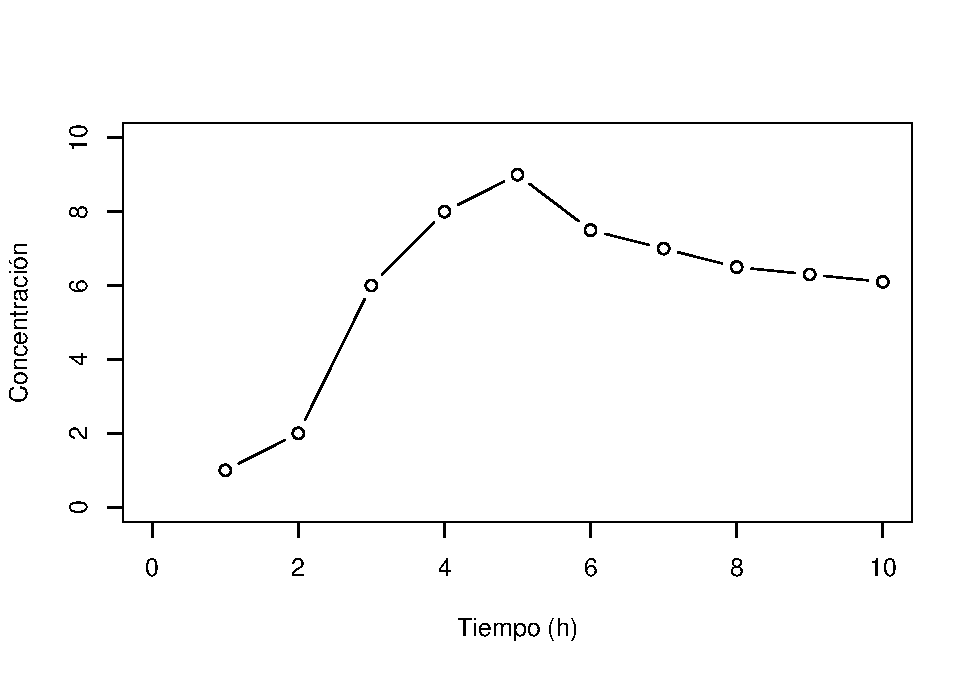
\includegraphics{fig_out/unnamed-chunk-2-1.pdf}

\begin{itemize}
\tightlist
\item
  Ver si la \textbf{evolución de una variable a lo largo del tiempo es la misma en diferentes grupos}. Por ejemplo ver si la concentración de un fármaco evoluaciona de la misma manera que otro fármaco ó placebo.
\end{itemize}

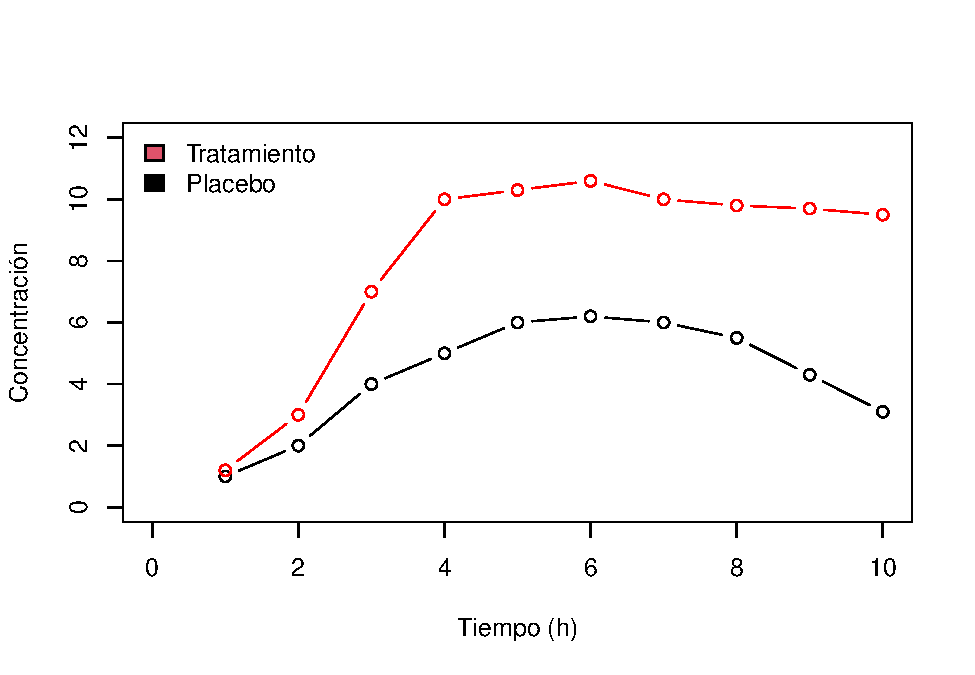
\includegraphics{fig_out/unnamed-chunk-3-1.pdf}

\begin{itemize}
\tightlist
\item
  \textbf{Identificar patrones en la evolución} o cambio de una variable a lo largo del tiempo. En este contexto se pueden usar técnicas basadas en las distancias entre curvas (que no se explicarán en este curso).
\end{itemize}

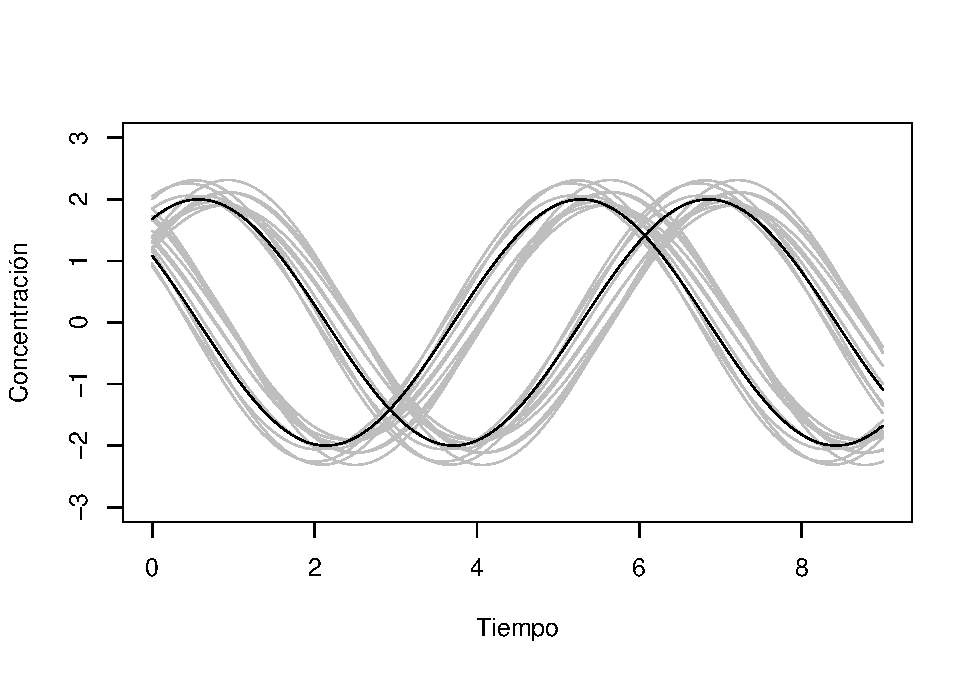
\includegraphics{fig_out/unnamed-chunk-4-1.pdf}

\hypertarget{ejemplos}{%
\section{Ejemplos}\label{ejemplos}}

\textbf{Ejemplo 1}

\begin{quote}
En un estudio de intervención de dieta se reclutan 100 individuos por grupo. Estos grupos son (1) grupo control: se sigue una dieta mediterránea; (2) grupo de frutos secos: la dieta mediterranea es complementada con una cantidad de nueces; (3) grupo de aceite de oliva: a la dieta mediterránea se le añade una cantidad de aceite de oliva virgen.
A lo largo de los siete años que dura el estudio, cada participante es visitado y se le toman distintas medidas desde cuestionarios de dieta, actividad física, medidas antropométricas (peso, talla), la tensión arterial, o medidas en sangre (perfil lipídico, etc.).
No todos los individuos acuden en todas las visitas con lo cual aparecen datos faltantes. Además, por motivos de enfermedad o de muerte, algunos de alguno de ellos no se tiene la información de las visitas finales, dando lugar a distintos tiempos de seguimiento.
\end{quote}

\textbf{Ejemplo 2}

\begin{quote}
A fin de comparar tres medicamentos (A, B y C) para reducir el colesterol, se reclutan 30 voluntarios, todos ellos diagnosticados de hipercolesterolemia y de entre 40 y 60 años de edad. Cada partipante se le asigna uno de los tres medicamentos al azar de forma que 10 de ellos toman el medicamento A, otros el medicamento B y los 10 restantes el medicamento C.

Se miden los niveles de colesterol total en sangre (en mg/dL) justo en el inicio del estudio y cada 7 días en ayunas, a lo largo de 12 semanas.
\end{quote}

\textbf{Ejemplo 3}

\begin{quote}
En un estudio sobre la polución ambiental en zonas urbanas, se eligen al azar 15 ciudades de más de 100.000 habitantes. De cada ciudad se eligen 4 puntos al azar con alta densidad de tráfico.

En cada punto se realizan 10 medidas desde las 8h de la mañana hasta las 17h de la tarde con intervalos de 60 minutos, en un día entre semana.
\end{quote}

\textbf{Ejemplo 4}

\begin{quote}
Se quiere estudiar la población de una especie de alga en aguas marinas poco profundas.
Para ello se muestrean veinte puntos al azar lo largo de la costa y a una distancia de aproximadamente un quilómetro de la playa. En cada punto se recoge una muestra a dos, cuatro, seis, ocho y diez metros de profundidas.

Finalmente, en cada muestra se contabilizan el número de especímenes que hay por centímetro cúbico de agua.
\end{quote}

\textbf{Ejemplo 5}

\begin{quote}
En un estudio farmacocinético, se inyecta una cierta cantidad de un componente farmacológico en sangre. Se reclutan 15 individuos y para cada uno de ellos se mide cada hora la concentración en sangre.

Se puede estudiar las características de la curva de la concentración a lo largo del tiempo resumiendo todos los datos de concentración en un solo valor como es el AUC, o el tiempo de inflexión, etc. O bien, se puede analizar la concentración en cada punto desde el punto de vista de medidas repetidas.

Este ejemplo también se podría tratar como análisis funcional, viendo los datos de cada individuo como una función del tiempo.
\end{quote}

\textbf{Ejemplo 6}

\begin{quote}
En un estudio sobre la adherencia a un medicamento, se hacen visitas mensuales a los participantes y en cada visita se pregunta si toma o no el medicamento con las dosis adecuadas, siendo la variable medida binaria (sí/no).
\end{quote}

\textbf{Ejemplo 7}

\begin{quote}
En un estudio se quiere ver la eficacia de una dieta rica en aceite de oliva sobre los niveles de colesterol triglicéridos.
Para ello se reculatan 3,000 participantes que son aleatorizados al grupo de tratamiento basado en una dieta enriquecida con aceite de oliva y a un grupo control a los que sólo se les indica que sigan una dieta saludable y pobre en grasas.
Cada participante se visita anualmente durante sieta años en que se mide, entre otras variables los niveles de triglicéridos. A fin de asegurar o evaluar hasta qué punto los participantes siguen la dieta que les ha tocado, también se mide en cada visita un parámetro en sangre sensible a la cantidad de aceite de oliva ingerido.
\end{quote}

\textbf{No serían medidas repetidas:}

\begin{quote}
\begin{enumerate}
\def\labelenumi{\arabic{enumi}.}
\tightlist
\item
  Expresión génica de distintos genes. En este ejemplo cada gen sería una variable distinta; nos podría interesar comparar los niveles de expresión entre distintos genes. Éste sería un ejemplo de muchas variables respuesta.
\end{enumerate}
\end{quote}

\begin{quote}
\begin{enumerate}
\def\labelenumi{\arabic{enumi}.}
\setcounter{enumi}{1}
\tightlist
\item
  Datos de seguimiento en el que se quiere estudiar la incidencia de diabetes. Para ello se hacen distintas visitas y se reporta en cada visita si el paciente es diabético o no. En este ejemplo, cada medida se toma o se mide si y solo si en la medida anterior el resultado es negativo. Sería un ejemplo de análisis de supervivencia con tiempo discreto.
\end{enumerate}
\end{quote}

\begin{quote}
\begin{enumerate}
\def\labelenumi{\arabic{enumi}.}
\setcounter{enumi}{2}
\tightlist
\item
  Si tenemos sólo dos medidas, aunque estrictamente son medidas repetidas, se pueden usar técnicas y modelos estándard. Por ejemplo, si la variable es continua se puede trabajar con la diferencia (después - antes) como la varaible respuesta y ajustar por el valor basal.
\end{enumerate}
\end{quote}

\begin{quote}
\begin{enumerate}
\def\labelenumi{\arabic{enumi}.}
\setcounter{enumi}{3}
\tightlist
\item
  Si tenemos distintas medidas pero no sabemos cuando o en qué orden se han recogido. Por ejemplo, si tenemos 3 medidas de tensión arterial para cada individuo pero no sabemos el orden en que se han tomado las medidas. En este caso, se trataría o analizaría como datos en clúster. Alternativamente se puede calcular la media para cada individuo y trabajar con modelo estándar con un sólo dato por individuo.
\end{enumerate}
\end{quote}

\hypertarget{esquemas-de-recogidas-de-datos}{%
\section{Esquemas de recogidas de datos}\label{esquemas-de-recogidas-de-datos}}

\hypertarget{todas-las-medidas-con-intervalos-fijos}{%
\subsection{Todas las medidas con intervalos fijos}\label{todas-las-medidas-con-intervalos-fijos}}

Medidas tomadas en los momentos \(t_1\), \(t_2\), \ldots, \(t_5\). El intervalo transcurrido entre dos medidas puede ser constante o no. Pero son las mismas para todos los individuos. En caso que el intervalo no sea constante es importante anotar en qué momentos (segundos, minutos, horas, días, o metros\ldots) se han hecho las medidas.

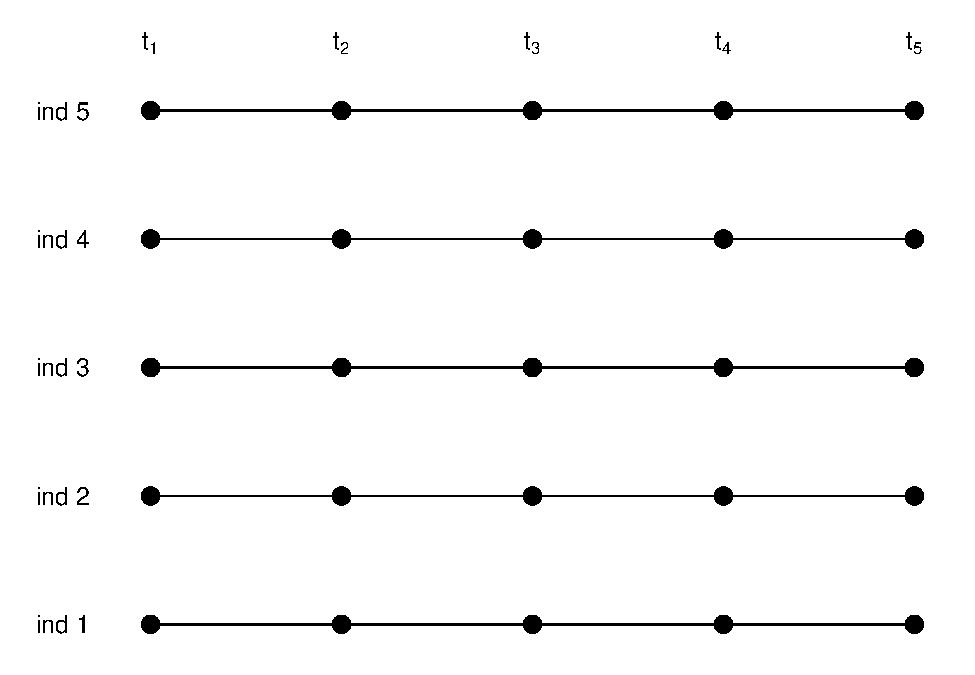
\includegraphics{fig_out/unnamed-chunk-5-1.pdf}

\hypertarget{missings-al-azar-con-intervalos-fijos}{%
\subsection{Missings al azar con intervalos fijos}\label{missings-al-azar-con-intervalos-fijos}}

No todos los individuos tienen datos observados en todos los tiempos. Es importante que estos datos faltantes ocurran al azar para poder considerar los modelos que vamos a ver en este curso como correctos.

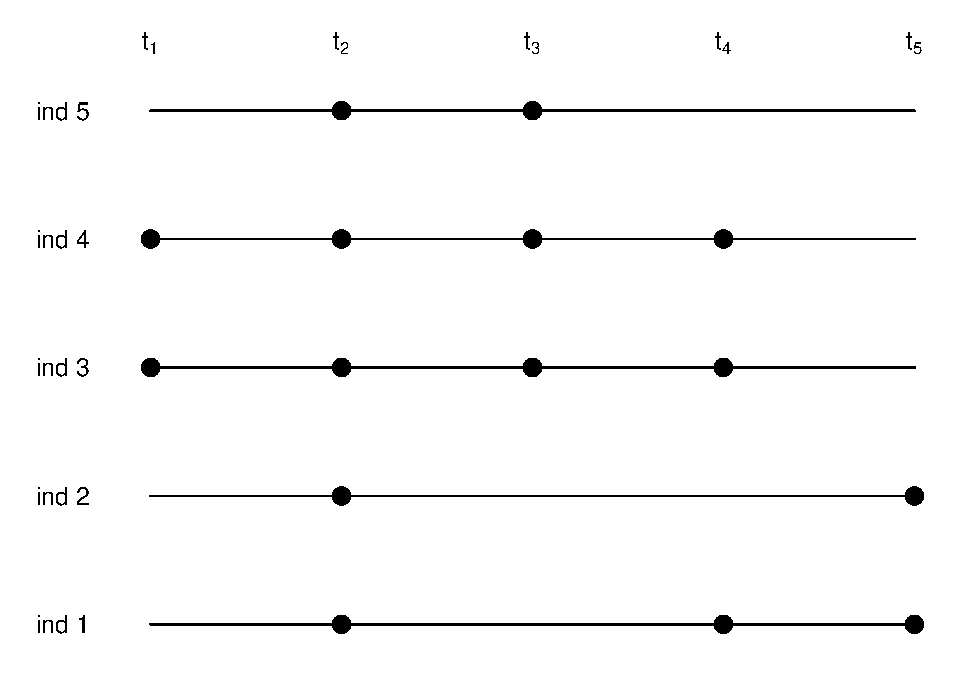
\includegraphics{fig_out/unnamed-chunk-6-1.pdf}

\hypertarget{distintos-seguimientos}{%
\subsection{Distintos seguimientos}\label{distintos-seguimientos}}

Algunos individuos son seguidos a lo largo del tiempo en más visitas que otros.

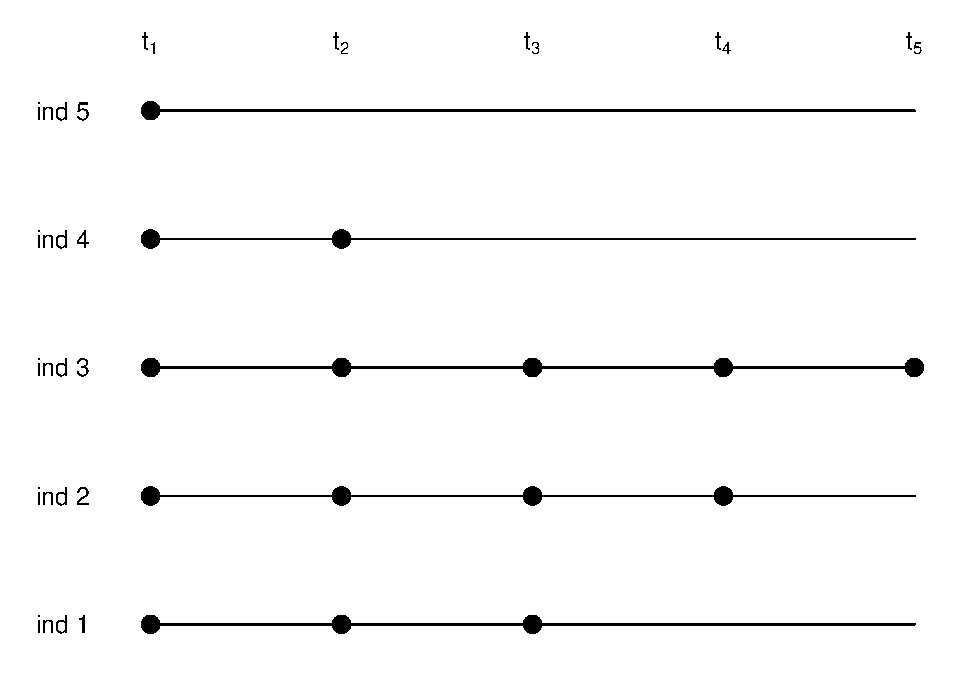
\includegraphics{fig_out/unnamed-chunk-7-1.pdf}

\hypertarget{todas-las-medidas-a-distintos-tiempos}{%
\subsection{Todas las medidas a distintos tiempos}\label{todas-las-medidas-a-distintos-tiempos}}

Los datos anteriores se consideran estudios de \textbf{datos panel}. Es decir, los datos se recogen de forma diara, semanal, anual, etc. (a tiempo fijo). Sin embargo, lo más habitual es disponer de observaciones en distintos tiempos para cada individuo y distintos número de observaciones para cada individuo.

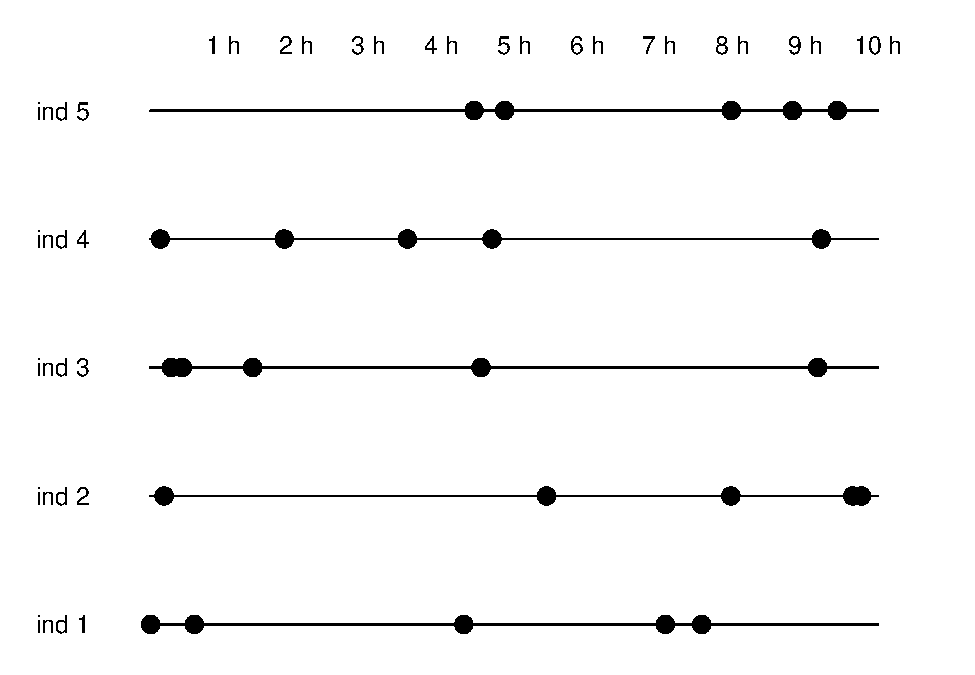
\includegraphics{fig_out/unnamed-chunk-8-1.pdf}

\hypertarget{estructura-de-los-datos}{%
\chapter{Estructura de los datos}\label{estructura-de-los-datos}}

\hypertarget{formato-ancho-y-largo}{%
\section{Formato ancho y largo}\label{formato-ancho-y-largo}}

Una vez que hemos recogido nuestros datos, debemos proceder con un análisis descriptivo para saber qué modelo debemos usar con el fin de contestar a las preguntas científicas planteadas en el estudio. La organización y visualización de los datos en estudios longitudinales no es tan sencilla como en cualquier otro tipo de diseño ya que los datos se pueden organizar de formas distintas. Básicamente, podemos:

\begin{itemize}
\item
  Datos a nivel de individuo, en el que cada individuo tiene un registro y múltiples variables contienen los datos de cada ocasión de medición (datos en formato ancho - \emph{wide format} en inglés).
\item
  Datos a nivel de tiempo, en el que cada persona tiene varios registros, uno para cada ocasión de medición (datos en formato largo - \emph{long format} en inglés).
\end{itemize}

Las funciones que tenemos en R tanto para visualizar como modelizar datos longitudinales puede requerir el tener los datos en cualquiera de los dos formatos. El formato largo normalmente se necesita para agrupar variables como por ejemplo si queremos visualizar nuestra información mediante gráficos de barras apilados. En R existen muchas funciones para pasar de formato ancho a largo y viceversa. Recientemente se han creado las fuciones \texttt{dcast()} y \texttt{melt()} en la librería \texttt{reshape2} que facilitan enormemente estas tareas. La siguiente figura muestra un ejemplo de cómo utilizar estas funciones:

\begin{figure}
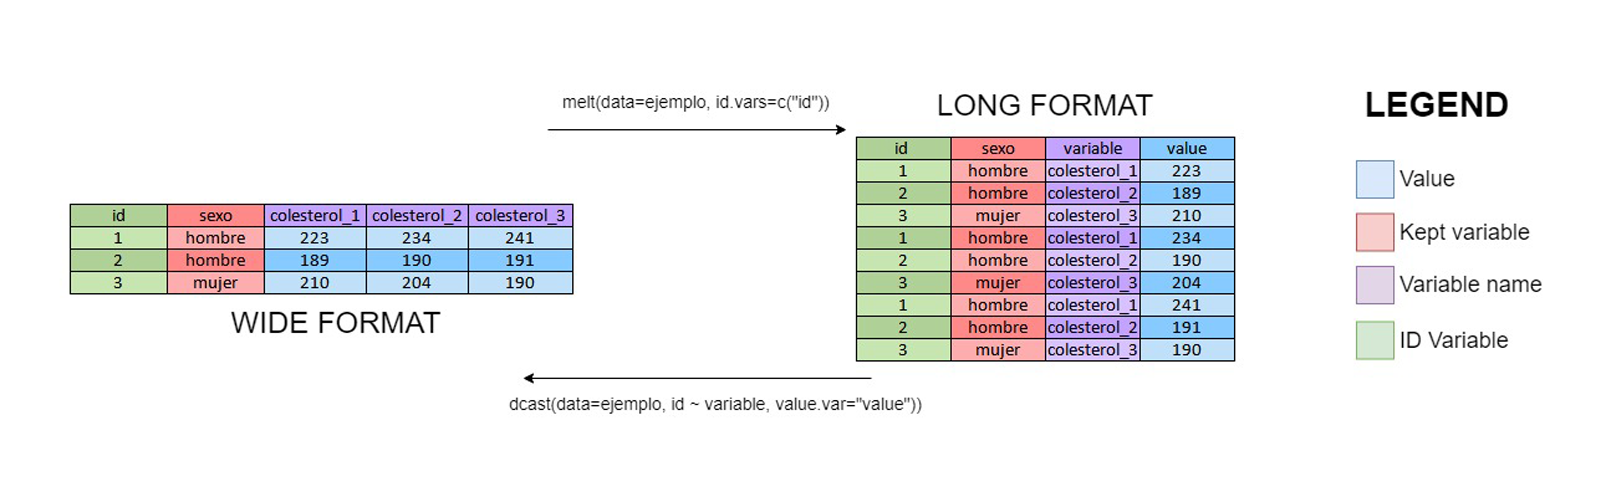
\includegraphics[width=22.22in]{fig/ejemplo_img_final} \caption{Datos en formato ancho y largo y cómo pasar de un formato a otro usando funciones de la librería `reshape2`}\label{fig:unnamed-chunk-9}
\end{figure}

Veamos cómo realizarlo con R. Empecemos por cargar los datos que hemos visto en el ejemplo anterior

\begin{Shaded}
\begin{Highlighting}[]
\NormalTok{datos }\OtherTok{\textless{}{-}} \FunctionTok{read.delim}\NormalTok{(}\StringTok{"datos/ejemplo.txt"}\NormalTok{)}
\NormalTok{datos}
\end{Highlighting}
\end{Shaded}

\begin{verbatim}
  id   sexo colesterol_1 colesterol_2
1  1 hombre          223          234
2  2 hombre          189          190
3  3  mujer          210          204
  colesterol_3
1          241
2          191
3          190
\end{verbatim}

Vemos que están en formato ancho. Podemos pasarlos a formato largo utilizando la función \texttt{melt()} que tiene los siguientes argumentos:

\begin{itemize}
\tightlist
\item
  \texttt{data} es el objeto (data.frame o tibble) que vamos a convertir de ancho a largo,
\item
  \texttt{id.vars} son las variables en la tabla que vamos a dejar sin cambiar de dimensión. En nuestro ejemplo sería la variable ``sexo'', aunque pueden ser más en tablas más complejas. Puede usarse un vector de nombres (tipo character) o de números enteros que correspondan al número de columna.
\item
  \texttt{measure.vars} son las variables en las que se encuentran las mediciones. Puede ser un vector de nombres o de números enteros indicando los índices de las columnas. En nuestro caso son las columnas 3 a 5.
\item
  \texttt{variable.name} es el nombre que va a adoptar la columna en la que queden nuestras variables, es decir, en nuestro caso sería el tiempo. Por defecto usa ``variable''.
\item
  \texttt{value.name} es el nombre que va a adoptar la columna en la que queden los valores, que en nuestro caso sería el colestero. Por defecto usa ``value''.
\item
  \texttt{variable.factor} es una valor lógico (TRUE o FALSE) para indicar si queremos que la columna de variable quede convertida a factor (opción por defecto), o quede simplemente como caracter.
\end{itemize}

Veamos cómo aplicamos esto a nuestro ejemplo

\begin{Shaded}
\begin{Highlighting}[]
\FunctionTok{library}\NormalTok{(reshape2)}
\NormalTok{datos\_largo }\OtherTok{\textless{}{-}} \FunctionTok{melt}\NormalTok{(datos, }\AttributeTok{measure.vars=}\DecValTok{3}\SpecialCharTok{:}\DecValTok{5}\NormalTok{,}
                    \AttributeTok{variable.name =} \StringTok{"tiempo"}\NormalTok{,}
                    \AttributeTok{value.name =} \StringTok{"colesterol"}\NormalTok{)}
\NormalTok{datos\_largo}
\end{Highlighting}
\end{Shaded}

\begin{verbatim}
  id   sexo       tiempo colesterol
1  1 hombre colesterol_1        223
2  2 hombre colesterol_1        189
3  3  mujer colesterol_1        210
4  1 hombre colesterol_2        234
5  2 hombre colesterol_2        190
6  3  mujer colesterol_2        204
7  1 hombre colesterol_3        241
8  2 hombre colesterol_3        191
9  3  mujer colesterol_3        190
\end{verbatim}

Notemos que nuestra variable \texttt{tiempo} no es numérica indicando el momento donde se toma la medida de colesterol. Debería de ser una variable numérica 1, 2, 3. Podemos solucionar esto eliminando ``colesterol\_'' de la variable simplemente ejecutando:

\begin{Shaded}
\begin{Highlighting}[]
\FunctionTok{library}\NormalTok{(tidyverse)}
\NormalTok{datos\_largo }\OtherTok{\textless{}{-}} \FunctionTok{mutate}\NormalTok{(datos\_largo, }
                      \AttributeTok{tiempo =} \FunctionTok{str\_remove}\NormalTok{(tiempo, }\StringTok{"colesterol\_"}\NormalTok{) }\SpecialCharTok{\%\textgreater{}\%}
                      \FunctionTok{as.numeric}\NormalTok{())}
\NormalTok{datos\_largo}
\end{Highlighting}
\end{Shaded}

\begin{verbatim}
  id   sexo tiempo colesterol
1  1 hombre      1        223
2  2 hombre      1        189
3  3  mujer      1        210
4  1 hombre      2        234
5  2 hombre      2        190
6  3  mujer      2        204
7  1 hombre      3        241
8  2 hombre      3        191
9  3  mujer      3        190
\end{verbatim}

Podemos ordenar nuestros datos por individuo y tiempo de la siguiente manera

\begin{Shaded}
\begin{Highlighting}[]
\NormalTok{datos\_largo }\OtherTok{\textless{}{-}} \FunctionTok{arrange}\NormalTok{(datos\_largo, id, tiempo)}
\NormalTok{datos\_largo}
\end{Highlighting}
\end{Shaded}

\begin{verbatim}
  id   sexo tiempo colesterol
1  1 hombre      1        223
2  1 hombre      2        234
3  1 hombre      3        241
4  2 hombre      1        189
5  2 hombre      2        190
6  2 hombre      3        191
7  3  mujer      1        210
8  3  mujer      2        204
9  3  mujer      3        190
\end{verbatim}

Veamos ahora cómo pasar de formato largo a ancho. Para esta tarea usamos la función \texttt{dcast()}. Esta función tiene una notación un poco diferente, pues usa fórmulas para determinar qué variables poner en cada lugar. Tiene los siguientes argumentos:

\begin{itemize}
\tightlist
\item
  \texttt{data} es la tabla que vamos a convertir,
\item
  \texttt{formula} es la forma en que vamos a distribuir las columnas. En general la fórmula es de forma x \textasciitilde{} y. Se puede usar una regla nemotécnica que consiste en: filas \textasciitilde{} columnas.
\item
  \texttt{drop} deberían los valores faltantes ser eliminados o mantenidos?. Por defecto es TRUE y no se ponen.
\item
  \texttt{value.var} es el nombre (o número) de la columna en la que están los valores. Generalmente \texttt{dcast()} adivina bien este valor, pero es bueno usarlo para asegurarnos de lo que estamos haciendo y evitar que salga un mensaje de advertencia.
\end{itemize}

En nuestro caso ejecutaríamos:

\begin{Shaded}
\begin{Highlighting}[]
\NormalTok{datos\_ancho }\OtherTok{\textless{}{-}} \FunctionTok{dcast}\NormalTok{(datos\_largo, id }\SpecialCharTok{\textasciitilde{}}\NormalTok{ tiempo,}
                     \AttributeTok{value.var =} \StringTok{"colesterol"}\NormalTok{)}
\NormalTok{datos\_ancho}
\end{Highlighting}
\end{Shaded}

\begin{verbatim}
  id   1   2   3
1  1 223 234 241
2  2 189 190 191
3  3 210 204 190
\end{verbatim}

Si queremos mantener el resto de covariables debemos ejecutar:

\begin{Shaded}
\begin{Highlighting}[]
\NormalTok{datos\_ancho }\OtherTok{\textless{}{-}} \FunctionTok{dcast}\NormalTok{(datos\_largo, id }\SpecialCharTok{+}\NormalTok{ sexo }\SpecialCharTok{\textasciitilde{}}\NormalTok{ tiempo, }
                     \AttributeTok{value.var =} \StringTok{"colesterol"}\NormalTok{)}
\NormalTok{datos\_ancho}
\end{Highlighting}
\end{Shaded}

\begin{verbatim}
  id   sexo   1   2   3
1  1 hombre 223 234 241
2  2 hombre 189 190 191
3  3  mujer 210 204 190
\end{verbatim}

que es justo el conjunto de datos inicial del que partíamos excepto por el nombre de las variables (que ahora se llaman 1, 2, 3). Para poder poner el nombre original, basta con ejecutar:

\begin{Shaded}
\begin{Highlighting}[]
\NormalTok{datos\_ancho }\OtherTok{\textless{}{-}} \FunctionTok{dcast}\NormalTok{(datos\_largo, id }\SpecialCharTok{+}\NormalTok{ sexo }\SpecialCharTok{\textasciitilde{}} \FunctionTok{paste0}\NormalTok{(}\StringTok{"colesterol\_"}\NormalTok{, tiempo), }
                     \AttributeTok{value.var =} \StringTok{"colesterol"}\NormalTok{)}
\NormalTok{datos\_ancho}
\end{Highlighting}
\end{Shaded}

\begin{verbatim}
  id   sexo colesterol_1 colesterol_2
1  1 hombre          223          234
2  2 hombre          189          190
3  3  mujer          210          204
  colesterol_3
1          241
2          191
3          190
\end{verbatim}

Veamos ahora ejemplos más reales donde tenemos más de una variable repetida a lo largo del tiempo, datos faltantes u datos recogidos en distintos tiempos.

\hypertarget{formato-ancho}{%
\section{Formato ancho}\label{formato-ancho}}

Como hemos comentado anteriormente, lo normal es recoger los datos en formato ancho (u horizontal) data su simplicidad.

ind

sexo

edad

coltot\_1

coltot\_2

coltot\_3

bmi\_1

bmi\_2

bmi\_3

1

1

44

213

220

199

33.3

30.9

28.3

2

0

45

196

238

218

31.1

29.1

30.1

3

1

55

195

218

216

28.5

30.0

27.9

4

0

51

201

194

201

32.5

31.4

24.5

5

1

46

234

185

189

30.1

31.9

27.7

6

0

51

213

183

214

30.4

28.8

28.3

La \textbf{ventaja} de esta estrategia es que tenemos una fila para cada individuo, como estamos acostumbrados.

Sin embargo, existen varios \textbf{inconvenientes}:

\begin{itemize}
\item
  Si tenemos un missing en alguna medida hay que eliminar a todo el individuo
\item
  Debemos suponer que todas las medidas se han realizado en los mismos momentos para todos los individuos, y esto puede no ser cierto.
\item
  Las diferentes medidas de una misma variable predictora la debemos analizar como si fueran distintas variables
\end{itemize}

\hypertarget{formato-largo}{%
\section{Formato largo}\label{formato-largo}}

Estos mismos datos se dispondrían de la siguiente forma en formato largo (o vertical)

ind

sexo

edad

coltot

bmi

momento

1

1

44

213

33.3

1

1

1

44

220

30.9

2

1

1

44

199

28.3

3

2

0

45

196

31.1

1

2

0

45

238

29.1

2

2

0

45

218

30.1

3

3

1

55

195

28.5

1

3

1

55

218

30.0

2

3

1

55

216

27.9

3

4

0

51

201

32.5

1

4

0

51

194

31.4

2

4

0

51

201

24.5

3

5

1

46

234

30.1

1

5

1

46

185

31.9

2

5

1

46

189

27.7

3

6

0

51

213

30.4

1

6

0

51

183

28.8

2

6

0

51

214

28.3

3

\hypertarget{valores-faltantes}{%
\section{Valores faltantes}\label{valores-faltantes}}

Cuando hay valores faltantes en una medida y los datos se disponen de forma horizontal se descartan los demás valores ya que se elimina toda la fila.

ind

sexo

edad

coltot\_1

coltot\_2

coltot\_3

bmi\_1

bmi\_2

bmi\_3

1

1

44

213

220

199

33.3

30.9

28.3

2

0

45

196

NA

218

31.1

29.1

30.1

3

1

55

195

218

216

28.5

30.0

27.9

4

0

51

201

194

201

32.5

31.4

24.5

5

1

46

234

185

NA

30.1

31.9

27.7

6

0

51

213

183

214

30.4

28.8

28.3

En cambio, en la disposición vertical sólo se pierden los valores de los tiempos en cuestión y no todas las medidas del individuo.

ind

sexo

edad

coltot

bmi

momento

1

1

44

213

33.3

1

1

1

44

220

30.9

2

1

1

44

199

28.3

3

2

0

45

196

31.1

1

2

0

45

NA

29.1

2

2

0

45

218

30.1

3

3

1

55

195

28.5

1

3

1

55

218

30.0

2

3

1

55

216

27.9

3

4

0

51

201

32.5

1

4

0

51

194

31.4

2

4

0

51

201

24.5

3

5

1

46

234

30.1

1

5

1

46

185

31.9

2

5

1

46

NA

27.7

3

6

0

51

213

30.4

1

6

0

51

183

28.8

2

6

0

51

214

28.3

3

\hypertarget{tiempos-de-medidas-diferentes}{%
\section{Tiempos de medidas diferentes}\label{tiempos-de-medidas-diferentes}}

Al disponer los datos de forma vertical se puede especificar en qué momento se ha recogido cada medida. Para ello simplemente se indica en la variable tiempo. Por ejemplo si se trata de los días que han pasado desde el momento inicial del experimento.

ind

sexo

edad

coltot

bmi

momento

dias

1

1

44

213

33.3

1

1

1

1

44

220

30.9

2

4

1

1

44

199

28.3

3

5

2

0

45

196

31.1

1

3

2

0

45

238

29.1

2

7

2

0

45

218

30.1

3

10

3

1

55

195

28.5

1

2

3

1

55

218

30.0

2

7

3

1

55

216

27.9

3

8

4

0

51

201

32.5

1

2

4

0

51

194

31.4

2

8

4

0

51

201

24.5

3

9

5

1

46

234

30.1

1

1

5

1

46

185

31.9

2

9

5

1

46

189

27.7

3

10

6

0

51

213

30.4

1

3

6

0

51

183

28.8

2

6

6

0

51

214

28.3

3

10

O incluso podemos tener mas medidas para unos individuos que para otros. Como sería el caso que tuviéramos algún missing en alguna medida. Como en este ejemplo, para el individuo 2 y el 5 tenemos sólo 2 medidas, mientras que para el resto tenemos 3.

ind

sexo

edad

coltot

bmi

momento

dias

1

1

44

213

33.3

1

1

1

1

44

220

30.9

2

4

1

1

44

199

28.3

3

5

2

0

45

196

31.1

1

3

2

0

45

218

30.1

3

10

3

1

55

195

28.5

1

2

3

1

55

218

30.0

2

7

3

1

55

216

27.9

3

8

4

0

51

201

32.5

1

2

4

0

51

194

31.4

2

8

4

0

51

201

24.5

3

9

5

1

46

234

30.1

1

1

5

1

46

185

31.9

2

9

6

0

51

213

30.4

1

3

6

0

51

183

28.8

2

6

6

0

51

214

28.3

3

10

\hypertarget{transformaciuxf3n}{%
\section{Transformación}\label{transformaciuxf3n}}

\hypertarget{vertical-a-horizontal-y-viceversa}{%
\subsection{Vertical a horizontal y viceversa}\label{vertical-a-horizontal-y-viceversa}}

En esta sección aprovecharemos para ver otras instrucciones útiles en \textbf{\texttt{R}} para pasar de la disposición vertical de los datos a la horizontal y viceversa (aunque yo recomiendo usar \texttt{melt()} y \texttt{dcast()}. Para ello usaremos los datos del ejemplo anterior que están guardados en formato .csv de la siguiente manera:

\begin{Shaded}
\begin{Highlighting}[]
\NormalTok{tablahorizontal }\OtherTok{\textless{}{-}} \FunctionTok{read.csv2}\NormalTok{(}\StringTok{"datos/tablahorizontal.csv"}\NormalTok{)}
\NormalTok{tablahorizontal}
\end{Highlighting}
\end{Shaded}

\begin{verbatim}
  ind sexo edad coltot_1 coltot_2 coltot_3 bmi_1
1   1    1   44      213      220      199  33.3
2   2    0   45      196      238      218  31.1
3   3    1   55      195      218      216  28.5
4   4    0   51      201      194      201  32.5
5   5    1   46      234      185      189  30.1
6   6    0   51      213      183      214  30.4
  bmi_2 bmi_3
1  30.9  28.3
2  29.1  30.1
3  30.0  27.9
4  31.4  24.5
5  31.9  27.7
6  28.8  28.3
\end{verbatim}

Como tenemos la base de datos en horizontal (una fila por individuo) y la queremos pasar a vertical (un registro por fila y varias filas por individuo) podemos usar:

\begin{Shaded}
\begin{Highlighting}[]
\NormalTok{tablong }\OtherTok{\textless{}{-}} \FunctionTok{reshape}\NormalTok{(}\AttributeTok{data=}\NormalTok{tablahorizontal, }
                   \AttributeTok{direction=}\StringTok{"long"}\NormalTok{, }
                   \AttributeTok{varying=}\FunctionTok{list}\NormalTok{(}\FunctionTok{c}\NormalTok{(}\StringTok{"coltot\_1"}\NormalTok{,}\StringTok{"coltot\_2"}\NormalTok{,}\StringTok{"coltot\_3"}\NormalTok{),}
                                \FunctionTok{c}\NormalTok{(}\StringTok{"bmi\_1"}\NormalTok{,}\StringTok{"bmi\_2"}\NormalTok{,}\StringTok{"bmi\_3"}\NormalTok{)), }
                   \AttributeTok{times=}\DecValTok{1}\SpecialCharTok{:}\DecValTok{3}\NormalTok{, }
                   \AttributeTok{timevar=}\StringTok{"momento"}\NormalTok{, }
                   \AttributeTok{idvar=}\StringTok{"ind"}\NormalTok{,}
                   \AttributeTok{v.names=}\FunctionTok{c}\NormalTok{(}\StringTok{"coltot"}\NormalTok{,}\StringTok{"bmi"}\NormalTok{))}
\NormalTok{tablong}
\end{Highlighting}
\end{Shaded}

\begin{verbatim}
    ind sexo edad momento coltot  bmi
1.1   1    1   44       1    213 33.3
2.1   2    0   45       1    196 31.1
3.1   3    1   55       1    195 28.5
4.1   4    0   51       1    201 32.5
5.1   5    1   46       1    234 30.1
6.1   6    0   51       1    213 30.4
1.2   1    1   44       2    220 30.9
2.2   2    0   45       2    238 29.1
3.2   3    1   55       2    218 30.0
4.2   4    0   51       2    194 31.4
5.2   5    1   46       2    185 31.9
6.2   6    0   51       2    183 28.8
1.3   1    1   44       3    199 28.3
2.3   2    0   45       3    218 30.1
3.3   3    1   55       3    216 27.9
4.3   4    0   51       3    201 24.5
5.3   5    1   46       3    189 27.7
6.3   6    0   51       3    214 28.3
\end{verbatim}

Ordeno la tabla por id y dentro de cada id por tiempo

\begin{Shaded}
\begin{Highlighting}[]
\NormalTok{tablong }\OtherTok{\textless{}{-}} \FunctionTok{arrange}\NormalTok{(tablong, ind, momento)}
\NormalTok{tablong}
\end{Highlighting}
\end{Shaded}

\begin{verbatim}
    ind sexo edad momento coltot  bmi
1.1   1    1   44       1    213 33.3
1.2   1    1   44       2    220 30.9
1.3   1    1   44       3    199 28.3
2.1   2    0   45       1    196 31.1
2.2   2    0   45       2    238 29.1
2.3   2    0   45       3    218 30.1
3.1   3    1   55       1    195 28.5
3.2   3    1   55       2    218 30.0
3.3   3    1   55       3    216 27.9
4.1   4    0   51       1    201 32.5
4.2   4    0   51       2    194 31.4
4.3   4    0   51       3    201 24.5
5.1   5    1   46       1    234 30.1
5.2   5    1   46       2    185 31.9
5.3   5    1   46       3    189 27.7
6.1   6    0   51       1    213 30.4
6.2   6    0   51       2    183 28.8
6.3   6    0   51       3    214 28.3
\end{verbatim}

Y si queremos pasar del formato largo al horizontal

\begin{Shaded}
\begin{Highlighting}[]
\NormalTok{tablavertical }\OtherTok{\textless{}{-}} \FunctionTok{read.csv2}\NormalTok{(}\StringTok{"datos/tablavertical.csv"}\NormalTok{)}
\NormalTok{tablavertical}
\end{Highlighting}
\end{Shaded}

\begin{verbatim}
   ind sexo edad coltot  bmi momento dias
1    1    1   44    213 33.3       1    1
2    1    1   44    220 30.9       2    4
3    1    1   44    199 28.3       3    5
4    2    0   45    196 31.1       1    3
5    2    0   45    238 29.1       2    7
6    2    0   45    218 30.1       3   10
7    3    1   55    195 28.5       1    2
8    3    1   55    218 30.0       2    7
9    3    1   55    216 27.9       3    8
10   4    0   51    201 32.5       1    2
11   4    0   51    194 31.4       2    8
12   4    0   51    201 24.5       3    9
13   5    1   46    234 30.1       1    1
14   5    1   46    185 31.9       2    9
15   5    1   46    189 27.7       3   10
16   6    0   51    213 30.4       1    3
17   6    0   51    183 28.8       2    6
18   6    0   51    214 28.3       3   10
\end{verbatim}

\begin{Shaded}
\begin{Highlighting}[]
\NormalTok{tabwide }\OtherTok{\textless{}{-}} \FunctionTok{reshape}\NormalTok{(}\AttributeTok{data=}\NormalTok{tablavertical, }
                   \AttributeTok{direction=}\StringTok{"wide"}\NormalTok{, }
                   \AttributeTok{v.names=}\FunctionTok{c}\NormalTok{(}\StringTok{"coltot"}\NormalTok{,}\StringTok{"bmi"}\NormalTok{), }
                   \AttributeTok{times=}\DecValTok{1}\SpecialCharTok{:}\DecValTok{3}\NormalTok{, }
                   \AttributeTok{timevar=}\StringTok{"momento"}\NormalTok{, }
                   \AttributeTok{idvar=}\StringTok{"ind"}\NormalTok{)}
\NormalTok{tabwide}
\end{Highlighting}
\end{Shaded}

\begin{verbatim}
   ind sexo edad dias coltot.1 bmi.1 coltot.2
1    1    1   44    1      213  33.3      220
4    2    0   45    3      196  31.1      238
7    3    1   55    2      195  28.5      218
10   4    0   51    2      201  32.5      194
13   5    1   46    1      234  30.1      185
16   6    0   51    3      213  30.4      183
   bmi.2 coltot.3 bmi.3
1   30.9      199  28.3
4   29.1      218  30.1
7   30.0      216  27.9
10  31.4      201  24.5
13  31.9      189  27.7
16  28.8      214  28.3
\end{verbatim}

¿Y si tenemos algun individuo con menos medidas? Por ejemplo, tenemos la tabla en formato vertical y para el individuo id=1 tenemos dos medidas en lugar de 3 (quitamos la tercera medida)

\begin{Shaded}
\begin{Highlighting}[]
\NormalTok{tablaverticalmiss }\OtherTok{\textless{}{-}}\NormalTok{ tablavertical[}\SpecialCharTok{{-}}\DecValTok{3}\NormalTok{,]}
\NormalTok{tablaverticalmiss}
\end{Highlighting}
\end{Shaded}

\begin{verbatim}
   ind sexo edad coltot  bmi momento dias
1    1    1   44    213 33.3       1    1
2    1    1   44    220 30.9       2    4
4    2    0   45    196 31.1       1    3
5    2    0   45    238 29.1       2    7
6    2    0   45    218 30.1       3   10
7    3    1   55    195 28.5       1    2
8    3    1   55    218 30.0       2    7
9    3    1   55    216 27.9       3    8
10   4    0   51    201 32.5       1    2
11   4    0   51    194 31.4       2    8
12   4    0   51    201 24.5       3    9
13   5    1   46    234 30.1       1    1
14   5    1   46    185 31.9       2    9
15   5    1   46    189 27.7       3   10
16   6    0   51    213 30.4       1    3
17   6    0   51    183 28.8       2    6
18   6    0   51    214 28.3       3   10
\end{verbatim}

\begin{Shaded}
\begin{Highlighting}[]
\NormalTok{tabwidemiss }\OtherTok{\textless{}{-}} \FunctionTok{reshape}\NormalTok{(}\AttributeTok{data=}\NormalTok{tablaverticalmiss, }
                       \AttributeTok{direction=}\StringTok{"wide"}\NormalTok{, }
                       \AttributeTok{v.names=}\FunctionTok{c}\NormalTok{(}\StringTok{"coltot"}\NormalTok{,}\StringTok{"bmi"}\NormalTok{), }
                       \AttributeTok{times=}\DecValTok{1}\SpecialCharTok{:}\DecValTok{3}\NormalTok{, }
                       \AttributeTok{timevar=}\StringTok{"momento"}\NormalTok{, }
                       \AttributeTok{idvar=}\StringTok{"ind"}\NormalTok{)}
\NormalTok{tabwidemiss}
\end{Highlighting}
\end{Shaded}

\begin{verbatim}
   ind sexo edad dias coltot.1 bmi.1 coltot.2
1    1    1   44    1      213  33.3      220
4    2    0   45    3      196  31.1      238
7    3    1   55    2      195  28.5      218
10   4    0   51    2      201  32.5      194
13   5    1   46    1      234  30.1      185
16   6    0   51    3      213  30.4      183
   bmi.2 coltot.3 bmi.3
1   30.9       NA    NA
4   29.1      218  30.1
7   30.0      216  27.9
10  31.4      201  24.5
13  31.9      189  27.7
16  28.8      214  28.3
\end{verbatim}

\hypertarget{colapsar}{%
\subsection{Colapsar}\label{colapsar}}

Si tenemos los datos en vertical y queremos colapsar o resumir los distintos datos de cada individuo en un único valor, como por ejemplo la media.

\begin{Shaded}
\begin{Highlighting}[]
\FunctionTok{library}\NormalTok{(dplyr) }
\FunctionTok{library}\NormalTok{(magrittr)}

\FunctionTok{group\_by}\NormalTok{(tablavertical, ind) }\SpecialCharTok{\%\textgreater{}\%}
  \FunctionTok{summarise\_at}\NormalTok{(}\FunctionTok{vars}\NormalTok{(coltot, bmi), }\FunctionTok{list}\NormalTok{(}\AttributeTok{media =}\NormalTok{ mean))}
\end{Highlighting}
\end{Shaded}

\begin{verbatim}
# A tibble: 6 x 3
    ind coltot_media bmi_media
  <int>        <dbl>     <dbl>
1     1         211.      30.8
2     2         217.      30.1
3     3         210.      28.8
4     4         199.      29.5
5     5         203.      29.9
6     6         203.      29.2
\end{verbatim}

\hypertarget{visualizaciuxf3n-de-datos-longitudinales}{%
\chapter{Visualización de datos longitudinales}\label{visualizaciuxf3n-de-datos-longitudinales}}

Para ilustrar cómo visualizar datos longitudinales usaremos los datos que se encuentran en formato ancho obtenidos de \href{https://stats.idre.ucla.edu/r/examples/alda/r-applied-longitudinal-data-analysis-ch-2/}{UCLA web site}. Este ejemplo pertenece a un estudio realizado en adolescentes en el que se ha medido su tolerancia a tener un comportamiento que se ``desvía de lo habitual'' usando 9 ítems (medidos en una escala de 1 a 4 que va de un comportamiento muy malo hasta para nada malo) que se resumen con la media del valor obtenido en cada uno de ellos. Además del sexo del adolescente, también se ha recogido una variable (``exposure'') que corresponde a la respuesta autoreportada por el adolescente a los 11 años de su exposición a tener un comportamiento que anómalo.

Los datos podemos cargarlos de la forma habitual, pero teniendo en cuenta que se encuentran en formato ``csv''. Notemos que no hace falta descargarlos en nuestro ordenador y cargarlos desde ahí, ya que la función \texttt{read\_csv} acepta que los datos estén en un repositorio en la red (basta con indicar su URL).

\begin{Shaded}
\begin{Highlighting}[]
\FunctionTok{library}\NormalTok{(tidyverse)}
\NormalTok{tolerance }\OtherTok{\textless{}{-}} \FunctionTok{read\_csv}\NormalTok{(}\StringTok{"https://stats.idre.ucla.edu/wp{-}content/uploads/2016/02/tolerance1.txt"}\NormalTok{)}
\FunctionTok{head}\NormalTok{(tolerance)}
\end{Highlighting}
\end{Shaded}

\begin{verbatim}
# A tibble: 6 x 8
     id tol11 tol12 tol13 tol14 tol15  male
  <dbl> <dbl> <dbl> <dbl> <dbl> <dbl> <dbl>
1     9  2.23  1.79  1.9   2.12  2.66     0
2    45  1.12  1.45  1.45  1.45  1.99     1
3   268  1.45  1.34  1.99  1.79  1.34     1
4   314  1.22  1.22  1.55  1.12  1.12     0
5   442  1.45  1.99  1.45  1.67  1.9      0
6   514  1.34  1.67  2.23  2.12  2.44     1
# ... with 1 more variable: exposure <dbl>
\end{verbatim}

Con los datos en este formato, podemos aprovechar para obtener algunas estadísticas descriptivas que pueden resultar de interés. Por ejemplo, podemos ver cuántos individuos tenemos en nuestro estudio simplemente ejecutando:

\begin{Shaded}
\begin{Highlighting}[]
\FunctionTok{nrow}\NormalTok{(tolerance)}
\end{Highlighting}
\end{Shaded}

\begin{verbatim}
[1] 16
\end{verbatim}

\hypertarget{trayectorias}{%
\section{Trayectorias}\label{trayectorias}}

Para poder crear gráficos que nos informen sobre la evolución de la tolerancia entre individuos necesitamos que los datos estén en formato largo. Como hemos visto anteriormente, esto lo podemos realizar mediante

\begin{Shaded}
\begin{Highlighting}[]
\FunctionTok{library}\NormalTok{(reshape2)}
\NormalTok{tolerance2 }\OtherTok{\textless{}{-}} \FunctionTok{melt}\NormalTok{(tolerance, }\AttributeTok{measure.vars=}\DecValTok{2}\SpecialCharTok{:}\DecValTok{6}\NormalTok{,}
                    \AttributeTok{variable.name =} \StringTok{"age"}\NormalTok{,}
                    \AttributeTok{value.name =} \StringTok{"tolerance"}\NormalTok{)}
\CommentTok{\# no nos olvidemos que nuestra variable edad}
\CommentTok{\# debe de ser numérica}
\NormalTok{tolerance2 }\OtherTok{\textless{}{-}} \FunctionTok{mutate}\NormalTok{(tolerance2, }
                     \AttributeTok{age =} \FunctionTok{str\_remove}\NormalTok{(age,}\StringTok{"tol"}\NormalTok{)}\SpecialCharTok{\%\textgreater{}\%}
                        \FunctionTok{as.numeric}\NormalTok{())}
\FunctionTok{head}\NormalTok{(tolerance2)}
\end{Highlighting}
\end{Shaded}

\begin{verbatim}
   id male exposure age tolerance
1   9    0     1.54  11      2.23
2  45    1     1.16  11      1.12
3 268    1     0.90  11      1.45
4 314    0     0.81  11      1.22
5 442    0     1.13  11      1.45
6 514    1     0.90  11      1.34
\end{verbatim}

Puesto que nuestras observaciones para cada individuo se presenta a distintas edades, por eso hemos llamado \texttt{age} a nuestra variable temporal.

Con los datos en este formato no resulta tan sencillo saber cuántos individuos estamos analizando. Podemos usar \texttt{tidyverse} para obtener esta información

\begin{Shaded}
\begin{Highlighting}[]
\NormalTok{tolerance2 }\SpecialCharTok{\%\textgreater{}\%} 
  \FunctionTok{distinct}\NormalTok{(id) }\SpecialCharTok{\%\textgreater{}\%} 
  \FunctionTok{nrow}\NormalTok{()}
\end{Highlighting}
\end{Shaded}

\begin{verbatim}
[1] 16
\end{verbatim}

\textbf{NOTA:} Para aquellos que no realizaron el último curso de R en el que se explicó tidyverse, se puede consultar \href{https://isglobal-brge.github.io/Aprendizaje_Automatico_1/introducci\%C3\%B3n-a-tidyverse.html}{este material}.

Podemos empezar por visualizar nuestros datos creando lo que se conoce como \emph{Empirical growth plots} o que nos nuestra la secuencia de nuestra variable de interés a lo largo del tiempo para cada individuo. En nuestro paso pondremos \texttt{age} en el eje X y \texttt{tolerance} en el Y. Para ello utilizaremos la función \texttt{geom\_point()} y para crear el panel individual para cada sujeto usaremos \texttt{facet\_wrap()} ambas son funciones de la librería \texttt{ggplot2}.

\begin{Shaded}
\begin{Highlighting}[]
\FunctionTok{library}\NormalTok{(ggplot2)}
\FunctionTok{ggplot}\NormalTok{(tolerance2, }\FunctionTok{aes}\NormalTok{(}\AttributeTok{x =}\NormalTok{ age, }\AttributeTok{y =}\NormalTok{ tolerance)) }\SpecialCharTok{+}
  \FunctionTok{geom\_point}\NormalTok{() }\SpecialCharTok{+}
  \FunctionTok{facet\_wrap}\NormalTok{(}\SpecialCharTok{\textasciitilde{}}\NormalTok{id)}
\end{Highlighting}
\end{Shaded}

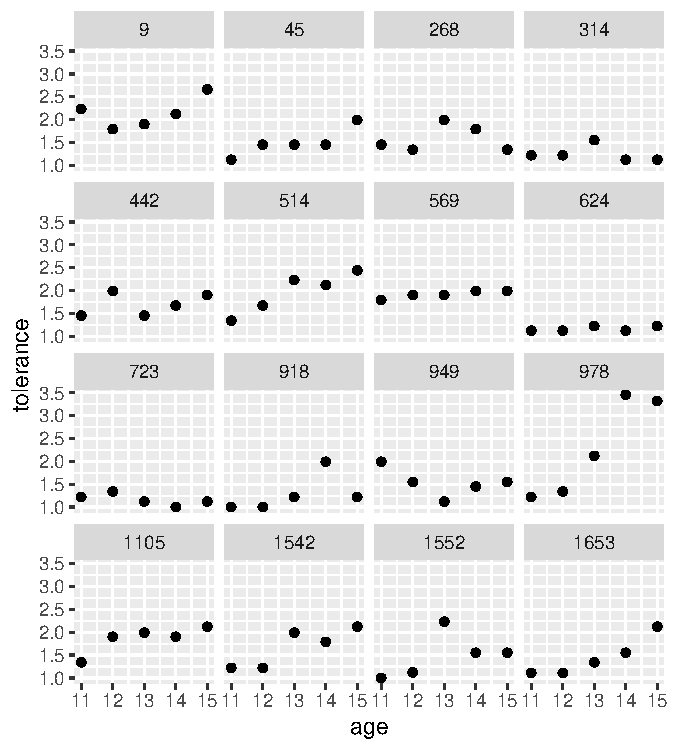
\includegraphics{fig_out/unnamed-chunk-35-1.pdf}

Por defecto, \texttt{ggplot2} mantiene las escalas de ambos ejes iguales en todos los paneles. Si queremos que sea distinto entre cada individuo, podemos modificar el argumento \texttt{scales} en la función \texttt{facet\_wrap()}.

Podemos añadir una línea para conectar los puntos usando \texttt{geom\_line()}

\begin{Shaded}
\begin{Highlighting}[]
\FunctionTok{ggplot}\NormalTok{(tolerance2, }\FunctionTok{aes}\NormalTok{(}\AttributeTok{x =}\NormalTok{ age, }\AttributeTok{y =}\NormalTok{ tolerance)) }\SpecialCharTok{+}
  \FunctionTok{geom\_point}\NormalTok{() }\SpecialCharTok{+}
  \FunctionTok{geom\_line}\NormalTok{() }\SpecialCharTok{+}
  \FunctionTok{facet\_wrap}\NormalTok{(}\SpecialCharTok{\textasciitilde{}}\NormalTok{id)}
\end{Highlighting}
\end{Shaded}

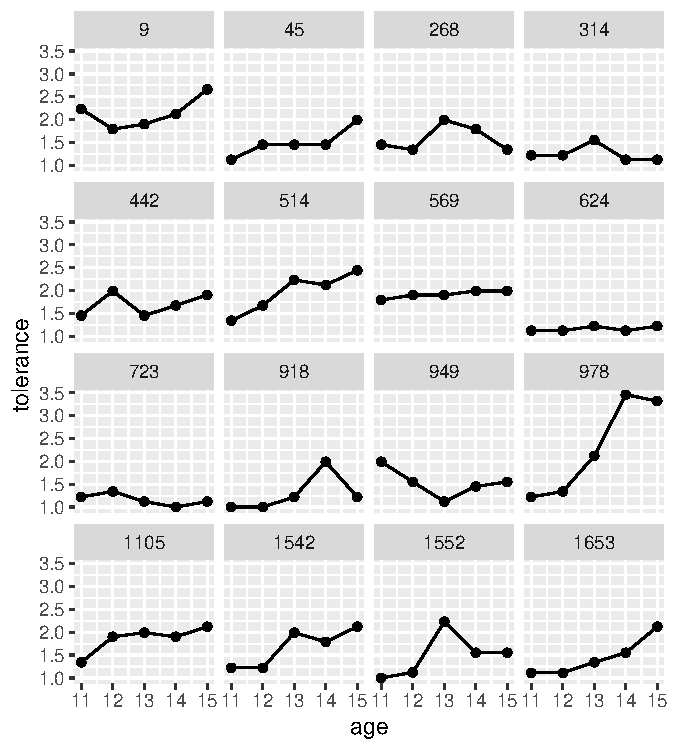
\includegraphics{fig_out/unnamed-chunk-36-1.pdf}

Sin embargo, a veces es recomendable utilizar otras aproximaciones que nos ayuden a visualizar mejor cuál es la trayectoria de cada individuo. Para ello, se puede utilizar otras aproximaciones como:

\begin{itemize}
\tightlist
\item
  suavizado no paramétrico
\item
  funciones paramétricas
\end{itemize}

El suavizado paramétrico se puede llevar acabo usando un suavizado de tipo \emph{loess}. Podemos usar esta opción mediante la función \texttt{stat\_smooth()} y controlar el grado de suavizado con el argumento \texttt{span}.

\begin{Shaded}
\begin{Highlighting}[]
\FunctionTok{ggplot}\NormalTok{(tolerance2, }\FunctionTok{aes}\NormalTok{(}\AttributeTok{x =}\NormalTok{ age, }\AttributeTok{y =}\NormalTok{ tolerance)) }\SpecialCharTok{+}
  \FunctionTok{geom\_point}\NormalTok{() }\SpecialCharTok{+}
  \FunctionTok{stat\_smooth}\NormalTok{(}\AttributeTok{method =} \StringTok{"loess"}\NormalTok{, }\AttributeTok{se =} \ConstantTok{FALSE}\NormalTok{, }\AttributeTok{span =}\NormalTok{ .}\DecValTok{9}\NormalTok{) }\SpecialCharTok{+}
  \FunctionTok{facet\_wrap}\NormalTok{(}\SpecialCharTok{\textasciitilde{}}\NormalTok{id)}
\end{Highlighting}
\end{Shaded}

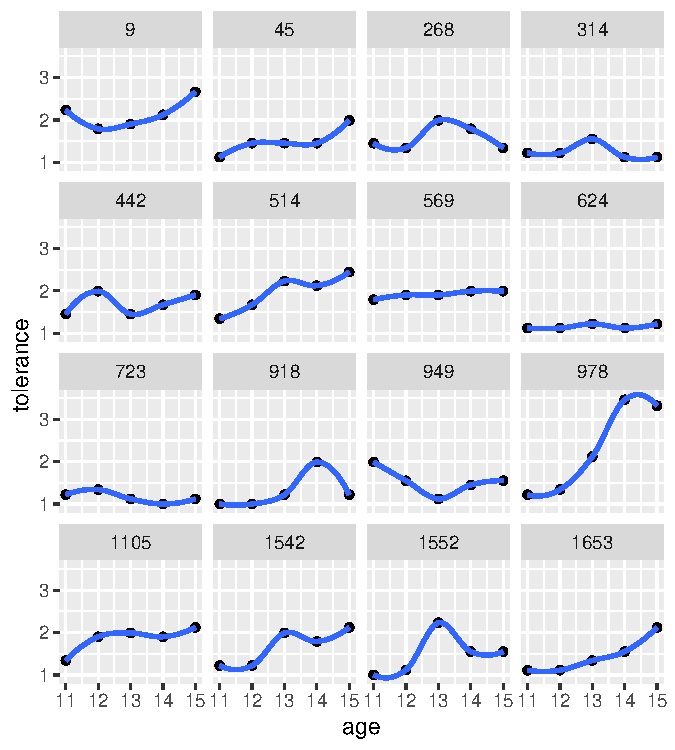
\includegraphics{fig_out/unnamed-chunk-37-1.pdf}
\textbf{NOTA:} El argumento \texttt{se=FALSE} sirve para que no pintemos la banda de confianza para la estimación no paramétrica.

Podemos visualizar las trayectorias usando un modelo paramétrico. El más sencillo sería un modelo lineal que podemos visualizar mediante el argumento \texttt{method\ =\ \textquotesingle{}lm\textquotesingle{}}

\begin{Shaded}
\begin{Highlighting}[]
\FunctionTok{ggplot}\NormalTok{(tolerance2, }\FunctionTok{aes}\NormalTok{(}\AttributeTok{x =}\NormalTok{ age, }\AttributeTok{y =}\NormalTok{ tolerance)) }\SpecialCharTok{+}
  \FunctionTok{geom\_point}\NormalTok{() }\SpecialCharTok{+}
  \FunctionTok{stat\_smooth}\NormalTok{(}\AttributeTok{method =} \StringTok{"lm"}\NormalTok{, }\AttributeTok{se =} \ConstantTok{FALSE}\NormalTok{) }\SpecialCharTok{+}
  \FunctionTok{facet\_wrap}\NormalTok{(}\SpecialCharTok{\textasciitilde{}}\NormalTok{id)}
\end{Highlighting}
\end{Shaded}

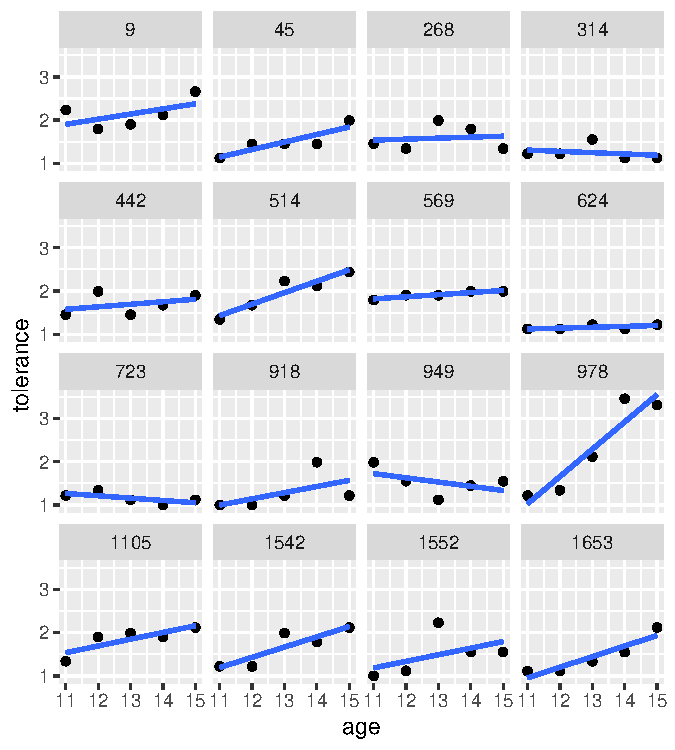
\includegraphics{fig_out/unnamed-chunk-38-1.pdf}

\hypertarget{spaghetti-plots}{%
\section{Spaghetti plots}\label{spaghetti-plots}}

También podemos visualizar todas las trayectorias en único gráfico mediante lo que se conoce como un \textbf{spaghetti plot}. Esta representación es muy útil cuando queremos visualizar muchos individuos. Para ello deberíamos usar el argumento \texttt{group}

\begin{Shaded}
\begin{Highlighting}[]
\FunctionTok{ggplot}\NormalTok{(tolerance2, }\FunctionTok{aes}\NormalTok{(}\AttributeTok{x =}\NormalTok{ age, }\AttributeTok{y =}\NormalTok{ tolerance, }\AttributeTok{group =}\NormalTok{ id)) }\SpecialCharTok{+}
  \FunctionTok{geom\_line}\NormalTok{()}
\end{Highlighting}
\end{Shaded}

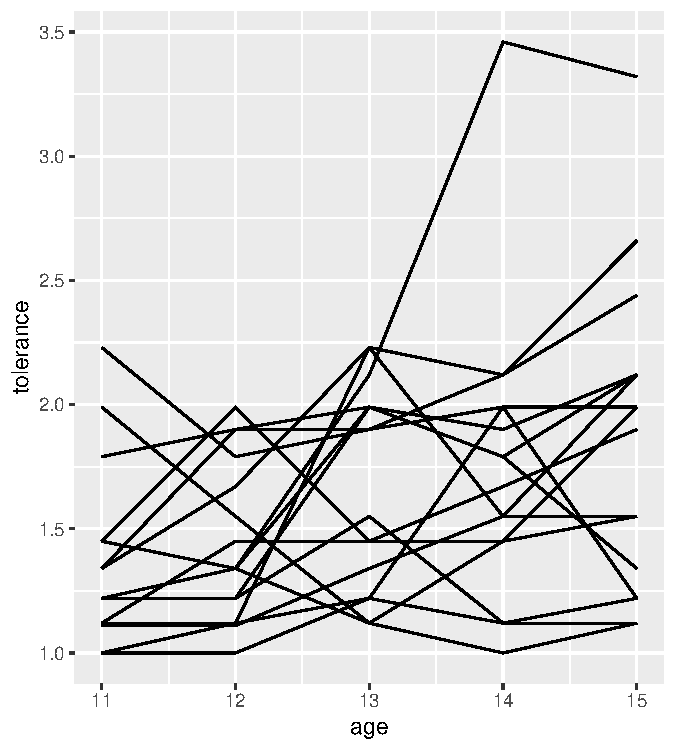
\includegraphics{fig_out/unnamed-chunk-39-1.pdf}

También podemos añadir el perfil promedio

\begin{Shaded}
\begin{Highlighting}[]
\FunctionTok{ggplot}\NormalTok{(tolerance2, }\FunctionTok{aes}\NormalTok{(}\AttributeTok{x =}\NormalTok{ age, }\AttributeTok{y =}\NormalTok{ tolerance, }\AttributeTok{group =}\NormalTok{ id)) }\SpecialCharTok{+}
  \FunctionTok{geom\_line}\NormalTok{(}\AttributeTok{col=}\StringTok{"grey"}\NormalTok{) }\SpecialCharTok{+} 
  \FunctionTok{stat\_summary}\NormalTok{(}\FunctionTok{aes}\NormalTok{(}\AttributeTok{group =} \DecValTok{1}\NormalTok{), }\AttributeTok{geom =} \StringTok{"line"}\NormalTok{, }\AttributeTok{fun =}\NormalTok{ mean, }\AttributeTok{size=}\DecValTok{2}\NormalTok{)}
\end{Highlighting}
\end{Shaded}

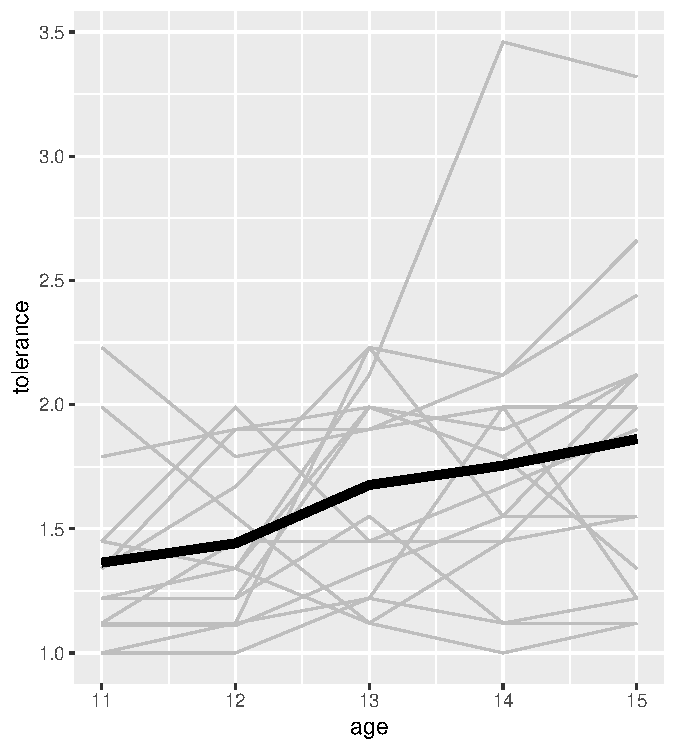
\includegraphics{fig_out/unnamed-chunk-40-1.pdf}

Podríamos obtener el mismo gráfico separado para hombres y mujeres usando de nuevo \texttt{facet\_wrap()}

\begin{Shaded}
\begin{Highlighting}[]
\FunctionTok{ggplot}\NormalTok{(tolerance2, }\FunctionTok{aes}\NormalTok{(}\AttributeTok{x =}\NormalTok{ age, }\AttributeTok{y =}\NormalTok{ tolerance, }\AttributeTok{group =}\NormalTok{ id)) }\SpecialCharTok{+}
  \FunctionTok{geom\_line}\NormalTok{() }\SpecialCharTok{+}
  \FunctionTok{facet\_wrap}\NormalTok{(}\SpecialCharTok{\textasciitilde{}}\NormalTok{male)}
\end{Highlighting}
\end{Shaded}

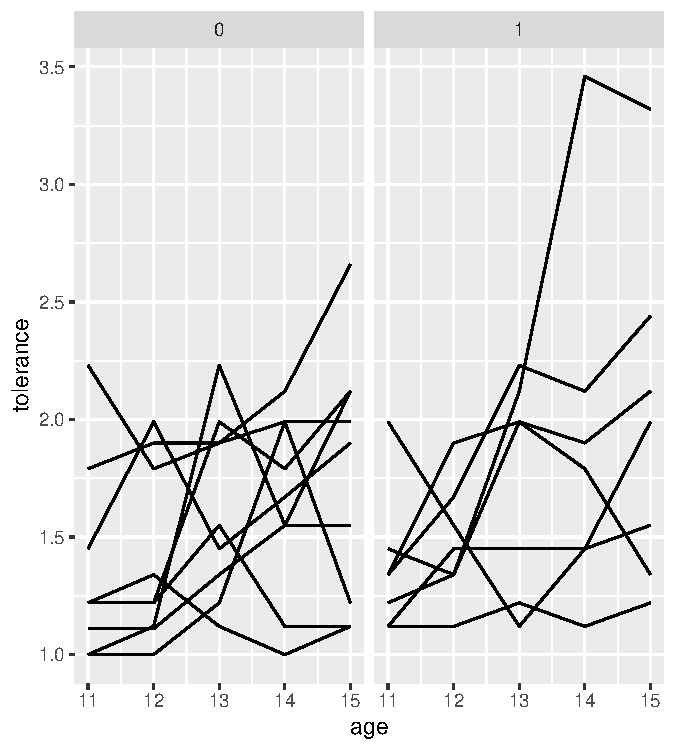
\includegraphics{fig_out/unnamed-chunk-41-1.pdf}

\textbf{NOTA:} En \texttt{ggplot2} podemos guardar un gráfico con un nombre y luego ``reciclar'' el gráfico añadiendo más código de la siguiente manera. Por ejemplo, puedo guardar el gráfico anterior en el objeto \texttt{p}

\begin{Shaded}
\begin{Highlighting}[]
\NormalTok{p }\OtherTok{\textless{}{-}} \FunctionTok{ggplot}\NormalTok{(tolerance2, }\FunctionTok{aes}\NormalTok{(}\AttributeTok{x =}\NormalTok{ age, }\AttributeTok{y =}\NormalTok{ tolerance, }\AttributeTok{group =}\NormalTok{ id)) }\SpecialCharTok{+}
  \FunctionTok{geom\_line}\NormalTok{(}\AttributeTok{col=}\StringTok{"gray"}\NormalTok{) }\SpecialCharTok{+}
  \FunctionTok{facet\_wrap}\NormalTok{(}\SpecialCharTok{\textasciitilde{}}\NormalTok{male)}
\end{Highlighting}
\end{Shaded}

y luego decirle que me añada el perfir promedio:

\begin{Shaded}
\begin{Highlighting}[]
\NormalTok{p }\SpecialCharTok{+} \FunctionTok{stat\_summary}\NormalTok{(}\FunctionTok{aes}\NormalTok{(}\AttributeTok{group =} \DecValTok{1}\NormalTok{),}
    \AttributeTok{geom =} \StringTok{"line"}\NormalTok{, }\AttributeTok{fun =}\NormalTok{ mean, }\AttributeTok{size=}\DecValTok{2}\NormalTok{)}
\end{Highlighting}
\end{Shaded}

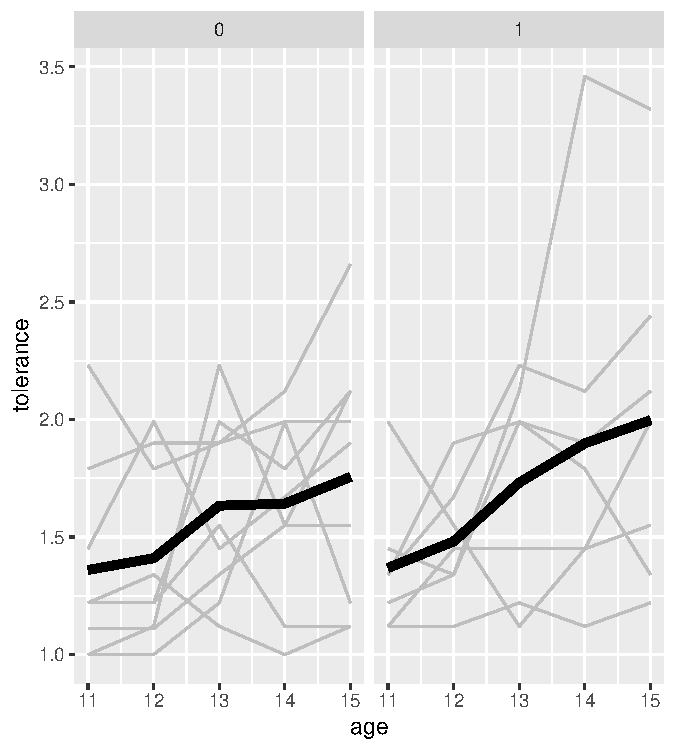
\includegraphics{fig_out/unnamed-chunk-43-1.pdf}

\hypertarget{ModelosNormal}{%
\chapter{Modelos con respuesta normal}\label{ModelosNormal}}

En este capítulo se describirán los métodos y modelos estadísticos para analizar medidas respetidas cuando la variable respuesta sigue una distribución normal o gaussiana. Se pueden probar algunas transformaciones, como el logaritmo, para normalizar la distribución de la variable.

\hypertarget{tuxe9cnica-de-la-suma-de-cuadrados}{%
\section{Técnica de la suma de cuadrados}\label{tuxe9cnica-de-la-suma-de-cuadrados}}

Este método o técnica se basa en la suma de cuadrados. Es la más simple desde el punto de vista estadístico y computacional. Por contra, sólo permite analizar diseños balanceados, sin variables independientes cuantitativas (covariables), sólo cualitativas o factores y con un número limitado de factores que tienen que estar cruzados (no anidados). A continuación se presentan los dos diseños más simples de medidas repetidas que se pueden analizar con esta técnica.

\hypertarget{diseuxf1o-1w1b}{%
\subsection{Diseño 1W+1B}\label{diseuxf1o-1w1b}}

Cuando el diseño es balanceado (mismo número de individuos por grupo), las medidas son las mismas para todos los individuos y no hay covariables, se puede usar la técnica de suma de cuadrados o tabla ANOVA.

La notación que se usa para la ecuación del modelo en el contexto de suma de cuadrados es:

\[y_{ijk} = \mu + \alpha_i + \beta_j + \alpha\beta_{ij} + \pi_{k(i)} + e_{ijk}\]

Donde

\begin{itemize}
\tightlist
\item
  \(\mu\) es la constante del modelo,
\item
  \(\alpha_i\), son los efectos del grupo o tratamiento
\item
  \(\beta_j\), son los efectos del tiempo
\item
  \(\alpha\beta_{ij}\) es la interacción del tiempo con el grupo
\item
  \(\pi_{k(i)}\) es el efecto aleatorio del individuo que está anidado al grupo
\item
  \(e_{ijk}\) son los errores
\end{itemize}

\(\sum_{i=1}^a \alpha_i=0\), \(\sum_{j=1}^b \beta_j=0\), \(\sum_{i=1}^a \alpha\beta_{ij}=0, \forall j\), \(\sum_{j=1}^b \alpha\beta_{ij}=0, \forall i\),

\(\pi_{k(i)} \sim N(0, \sigma_{ind})\)
\(e_{ijk} \sim N(0, \sigma)\) indep

En este contexto se dice que el tiempo y la interacción tratamiento:tiempo son términos o componentes ``intra sujeto'' (\emph{within subject}). Mientras que el grupo es un componente ``entre sujeto'' (\emph{between subject}). Por lo tanto, se trata de un diseño \textbf{1W+1B}.

Las técnicas clásicas de la tabla ANOVA y su inferencia són válidas siempre y cuando se cumpla la \textbf{condición de esfericidad}: la variancia de la diferencia entre dos medidas es constante. Para comprobar la condición de esfericidad se puede aplicar el \textbf{test de Mauchly}.

Si no se cumple hay que corregir los grados de libertad de los términos ``intra sujetos'' de la tabla ANOVA y se recalculan sus p-valores. Hay dos métodos para \textbf{corregir los grados de libertad}: método ``Huynh and Feldt'' (H-F) y el método ``Greenhouse-Geisser'' (G-G) .

\hypertarget{diseuxf1o-1w}{%
\subsection{Diseño 1W}\label{diseuxf1o-1w}}

Si en el diseño no hay grupos, luego el modelo se simplifica a un diseño de un solo factor ``intra sujeto'' \textbf{(1W)}

\[y_{ij} = \mu + \pi_i + \beta_j + e_{ij}\]

En ambos casos, tanto en el diseño en que tenemos grupos (1W+1B) como en el que no (1W), no nos interesa evaluar el efecto del individuo; ya sabemos que hay variabilidad entre ellos. Veremos en un ejemplo como el paquete \textbf{\texttt{ez}} que se usará para esta técnica de suma de cuadrados omite los resultados sobre el factor aleatorio individuo.

\hypertarget{funciuxf3n-ezanova}{%
\subsection{\texorpdfstring{Función \texttt{ezANOVA}}{Función ezANOVA}}\label{funciuxf3n-ezanova}}

Para ajustar los modelos de medidas repetidas balanceados mediante la técnica de suma de cuadrados existe la función \textbf{\texttt{ezANOVA}} del paquete \href{https://github.com/mike-lawrence/ez}{ez}.

\begin{Shaded}
\begin{Highlighting}[]
\FunctionTok{library}\NormalTok{(ez)}
\end{Highlighting}
\end{Shaded}

Tanto la corrección por H-F o G-G, como el test de esfericidad de Mauchly estan implementados en el package \texttt{ez} de R. Para visualizar gráficamente los resultados, se usará la función \texttt{ezPlot()}. Más adelante en esta sección se verá en un ejemplo de ambas funciones. Para llevar a cabo los análisis ANOVA se usa la función \texttt{ezANOVA\ ()} que tiene los siguientes argumentos:

\begin{itemize}
\item
  \texttt{data}: base de datos donde se encuentran las variables
\item
  \texttt{dv}: variable respuesta o variable dependiente
\item
  \texttt{wid}: variable individuo
\item
  \texttt{within}: factor o factores ``intra sujeto''. Típicamente en este argumento se espedificará el tiempo. Si se especifica más de un factor, éstos deben estar cruzados y se escribirá \texttt{.(var1,var2)}.
\item
  \texttt{between}: factor o factores ``entre sujetos''. Si no hay ningún factor ``intra-sujeto'' se deja a \texttt{NULL}. Como en el argumento \texttt{within}, si hay más de un factor ``entre sujetos'', éstos deben estar cruzados y se escribirá \texttt{.(var1,var2)}.
\end{itemize}

\textbf{Observaciones:}

\begin{itemize}
\tightlist
\item
  Los datos deben estar en formato vertical.
\item
  La variable respuesta y los factores deben escribirse sin comillas.
\item
  Los factores ``intra'', ``entre'' y el sujeto deben estar en format \texttt{factor}.
\item
  El factor individuo debe tener tantos niveles como individuos.
\item
  Aunque en teoría la función permite covariables (variables independientes contínuas), esta opción está en versión ``beta''.
\item
  Todos los factores, excepto el individuo, deben ser de efectos fijos.
\end{itemize}

\hypertarget{respuesta-multivariante}{%
\section{Respuesta Multivariante}\label{respuesta-multivariante}}

Esta metodología también conocida como MANOVA asume que las observaciones de cada individuo es un vector multivariante donde la variable respuesta se considera dicho vector. Podemos escribirlo de la siguiente forma:

\[\vec{y}_i = \vec{\mu}_i + \vec{e}_i\]

Donde

\begin{itemize}
\item
  \(\vec{y_i}=(y_{i1},\ldots,y_{iT})\) es el vector de medidas para el individuo \(i\).
\item
  \(\vec{\mu}_i=(\mu_{i1},\ldots,\mu_{iT})\) es el vector con las medias de cada momento y para cada individuo. Las medias pueden depender de las variables independientes \(x_k\). Fíjate que el coeficiente \(\beta_{kj}\) puede ser diferente para cada momento.
\end{itemize}

\[\mu_{ij} = \sum_{k=1}^K \beta_{jk} x_{ik}, \quad j=1,...,T\]

\begin{itemize}
\item
  \(\vec{e_i} \sim N(\vec{0},\Sigma)\), donde \(\Sigma\) es la matrix de covarianzas de los errores y tiene que ser la misma para todos los individuos. Su estructura, pero, puede ser cualquiera.
\item
  \(x_{ik}\) valor de la variable independiente \(k\) del individuo \(i\).
\end{itemize}

\textbf{Observaciones}

\begin{itemize}
\item
  Para ajustar este modelo los datos se disponen de forma horizontal (ancho).
\item
  En este modelo los tiempos en que se toman las \(T\) medidas tienen que ser los mismos para todos los individuos.
\item
  Para estudiar la evolución en el tiempo se puede realizar un contraste polinómico en el vector de medias \(\vec{\mu}\).
\item
  Para comparar grupos de medidas, por ejemplo si se tienen cinco medidas, las dos primeras corresponden al tratamiento A y las otras tres al tratamiento B, se puede realizar un contraste lineal para comparar los dos tratamientos.
\item
  Cuando hay un valor faltante en alguna medida, toda la fila del individuo se tiene que eliminar.
\item
  Cada variable independiente, \(x_{ki}\) es un único valor por individuo. O sea, que este modelo no contempla que las variables independientes sean de medidas repetidas. Si tuviéramos una variable que cambiara en el tiempo, se tienen que poner como variables diferentes (una para cada momento).
\item
  Los factores contribuyen con tantas dummy variables como categorías menos uno en los términos \(x_{ik}\).
\item
  Los términos \(x_{ik}\) pueden ser también interacciones entre variables, como el producto de sus términos.
\end{itemize}

Datos

Matriz de diseño \texttt{\textasciitilde{}\ fumador\ +\ edad\ +\ sexo\ +\ edad:fumador}

indiv

edad

fumador

sexo

fumadorEx

fumadorNunca

edad

sexomujer

fumadorEx:edad

fumadorNunca:edad

1

50

Ex

mujer

1

0

50

1

50

0

2

55

Actual

mujer

0

0

55

1

0

0

3

60

Actual

hombre

0

0

60

0

0

0

4

65

Nunca

mujer

0

1

65

1

0

65

5

62

Ex

hombre

1

0

62

0

62

0

\hypertarget{ejemplos-1}{%
\section{Ejemplos}\label{ejemplos-1}}

Vamos a ver algunos ejemplos que se analizarán mediante las técnicas que se acaban de describir.

\hypertarget{Ejemplo1}{%
\subsection{Ejemplo 1}\label{Ejemplo1}}

En la base de datos ``Ejemplo\_1W.csv'' se tienen los datos de un diseño con 12 individuos en los que se toman los niveles en sangre de un cierto parámetro lipídico. Para cada invidivuo se miden los niveles a 1, 2 y 3 horas.

\begin{Shaded}
\begin{Highlighting}[]
\NormalTok{datos }\OtherTok{\textless{}{-}} \FunctionTok{read.csv2}\NormalTok{(}\StringTok{"datos/Ejemplo\_1W.csv"}\NormalTok{)}
\end{Highlighting}
\end{Shaded}

Ordenamos por individuo y dentro por tiempo dentro de individuo

\begin{Shaded}
\begin{Highlighting}[]
\NormalTok{datos }\OtherTok{\textless{}{-}} \FunctionTok{arrange}\NormalTok{(datos, indiv, tiempo)}
\end{Highlighting}
\end{Shaded}

\hypertarget{exploraciuxf3n-de-los-datos}{%
\subsubsection{Exploración de los datos}\label{exploraciuxf3n-de-los-datos}}

\begin{Shaded}
\begin{Highlighting}[]
\FunctionTok{library}\NormalTok{(ggplot2)}
\NormalTok{p }\OtherTok{\textless{}{-}} \FunctionTok{ggplot}\NormalTok{(}\AttributeTok{data =}\NormalTok{ datos, }\FunctionTok{aes}\NormalTok{(}\AttributeTok{x =}\NormalTok{ tiempo, }\AttributeTok{y =}\NormalTok{ medida, }\AttributeTok{group =}\NormalTok{ indiv))}
\NormalTok{p }\SpecialCharTok{+} \FunctionTok{geom\_line}\NormalTok{(}\AttributeTok{col=}\StringTok{"grey"}\NormalTok{) }\SpecialCharTok{+} \FunctionTok{stat\_summary}\NormalTok{(}\FunctionTok{aes}\NormalTok{(}\AttributeTok{group =} \DecValTok{1}\NormalTok{),}
    \AttributeTok{geom =} \StringTok{"line"}\NormalTok{, }\AttributeTok{fun =}\NormalTok{ mean, }\AttributeTok{size=}\DecValTok{2}\NormalTok{)}
\end{Highlighting}
\end{Shaded}

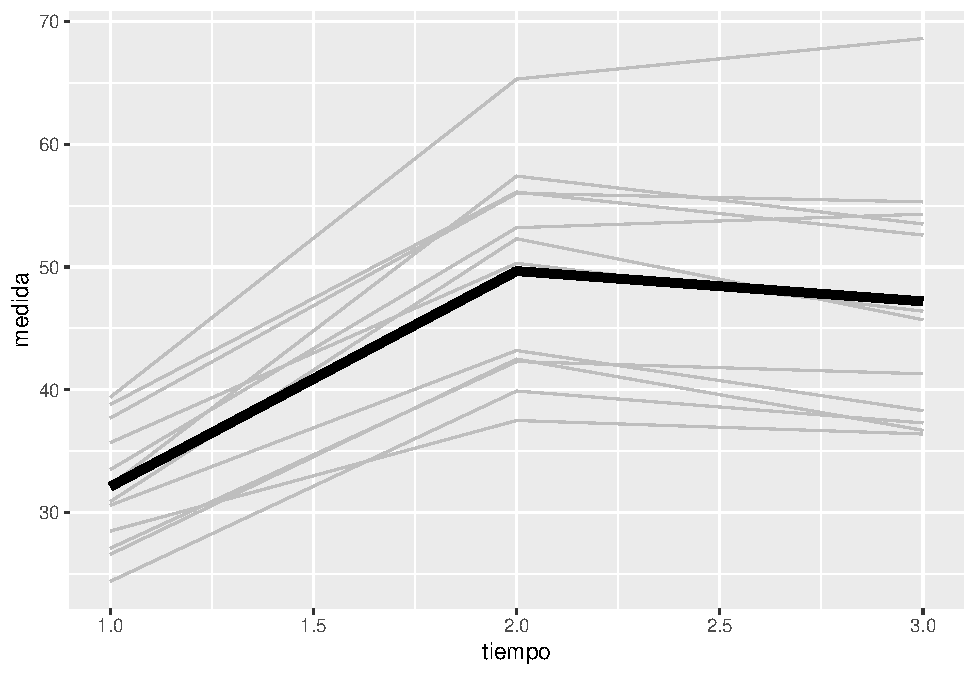
\includegraphics{fig_out/unnamed-chunk-48-1.pdf}

Cada línea representa a un individuo, mientras que la línea más gruesa es el promedio de los 12 individuos. Vemos como el efecto del tiempo no es del todo lineal. Además las líneas están bastante separadas indicando variabilidad entre los individuos.

Comprobemos si tenemos algún inviduo con datos faltantes

\begin{Shaded}
\begin{Highlighting}[]
\FunctionTok{sum}\NormalTok{(}\FunctionTok{with}\NormalTok{(datos, }\FunctionTok{tapply}\NormalTok{(}\FunctionTok{is.na}\NormalTok{(medida), indiv, any)))}
\end{Highlighting}
\end{Shaded}

\begin{verbatim}
[1] 0
\end{verbatim}

Como son datos balanceados, podemos usar ANOVA y MANOVA

\hypertarget{suma-de-cuadrados-anova}{%
\subsubsection{Suma de cuadrados (ANOVA)}\label{suma-de-cuadrados-anova}}

Para ajustar este modelo hay que usar los datos en disposición vertical.
Además, hay que convertir las variables \texttt{tiempo} e \texttt{indiv} a factor.

\begin{Shaded}
\begin{Highlighting}[]
\FunctionTok{library}\NormalTok{(ez)}

\NormalTok{datos.ez }\OtherTok{\textless{}{-}}\NormalTok{ datos}
\NormalTok{datos.ez}\SpecialCharTok{$}\NormalTok{tiempo }\OtherTok{\textless{}{-}} \FunctionTok{factor}\NormalTok{(datos.ez}\SpecialCharTok{$}\NormalTok{tiempo)}
\NormalTok{datos.ez}\SpecialCharTok{$}\NormalTok{indiv }\OtherTok{\textless{}{-}} \FunctionTok{factor}\NormalTok{(datos.ez}\SpecialCharTok{$}\NormalTok{indiv)}

\FunctionTok{ezANOVA}\NormalTok{(}\AttributeTok{data=}\NormalTok{datos.ez, }\AttributeTok{dv=}\NormalTok{medida, }\AttributeTok{wid=}\NormalTok{indiv, }\AttributeTok{within=}\NormalTok{tiempo, }\AttributeTok{detailed =} \ConstantTok{TRUE}\NormalTok{)}
\end{Highlighting}
\end{Shaded}

\begin{verbatim}
$ANOVA
       Effect DFn DFd       SSn       SSd
1 (Intercept)   1  11 66546.801 1892.0589
2      tiempo   2  22  2166.376  264.6244
          F            p p<.05       ges
1 386.88796 6.390053e-10     * 0.9686088
2  90.05264 2.542699e-11     * 0.5011210

$`Mauchly's Test for Sphericity`
  Effect         W          p p<.05
2 tiempo 0.4433135 0.01712201     *

$`Sphericity Corrections`
  Effect       GGe        p[GG] p[GG]<.05
2 tiempo 0.6423901 5.662497e-08         *
        HFe        p[HF] p[HF]<.05
2 0.6905331 1.998401e-08         *
\end{verbatim}

La condición de esfericidad no se cumple dado que el test de Mauchly es significativo. Por lo tanto, hay que corregir los grados de libertad y, en consecuencia, el p-valor del factor tiempo. Después de la corrección, éste sigue siendo significativo.

\hypertarget{modelo-de-respuesta-multivariante-manova}{%
\subsubsection{Modelo de respuesta multivariante (MANOVA)}\label{modelo-de-respuesta-multivariante-manova}}

Para analizar los datos mediante el modelo de respuesta multivariante hay que disponer los datos de forma horizontal.

\begin{Shaded}
\begin{Highlighting}[]
\NormalTok{datosh }\OtherTok{\textless{}{-}} \FunctionTok{dcast}\NormalTok{(datos, indiv }\SpecialCharTok{\textasciitilde{}} \FunctionTok{paste0}\NormalTok{(}\StringTok{"medida\_"}\NormalTok{, tiempo),}
                 \AttributeTok{value.var =} \StringTok{"medida"}\NormalTok{ )}
\NormalTok{datosh}
\end{Highlighting}
\end{Shaded}

\begin{verbatim}
   indiv medida_1 medida_2 medida_3
1      1     39.4     65.3     68.6
2      2     33.5     53.2     54.3
3      3     27.1     42.3     41.3
4      4     30.9     52.3     45.7
5      5     32.2     57.4     53.5
6      6     26.6     42.5     36.7
7      7     28.5     37.5     36.4
8      8     37.7     56.0     55.3
9      9     35.7     50.3     46.4
10    10     30.6     43.2     38.3
11    11     24.4     39.9     37.3
12    12     38.8     56.1     52.6
\end{verbatim}

Para ajustar un modelo de regresión lineal con respuesta multivariante se puede usar la función \texttt{lm}. Y hay que poner la variable respuesta a la izquierda de \texttt{\textasciitilde{}} como una matriz de las tres variables (\texttt{medida.1}, \texttt{medida.2} y \texttt{medida.3}):

\begin{Shaded}
\begin{Highlighting}[]
\NormalTok{respuesta }\OtherTok{\textless{}{-}} \FunctionTok{as.matrix}\NormalTok{(datosh[,}\FunctionTok{c}\NormalTok{(}\StringTok{"medida\_1"}\NormalTok{,}\StringTok{"medida\_2"}\NormalTok{,}\StringTok{"medida\_3"}\NormalTok{)])}
\NormalTok{modelo }\OtherTok{\textless{}{-}} \FunctionTok{lm}\NormalTok{(respuesta }\SpecialCharTok{\textasciitilde{}} \DecValTok{1}\NormalTok{, }\AttributeTok{data=}\NormalTok{datosh)}
\FunctionTok{class}\NormalTok{(modelo)}
\end{Highlighting}
\end{Shaded}

\begin{verbatim}
[1] "mlm" "lm" 
\end{verbatim}

\begin{Shaded}
\begin{Highlighting}[]
\FunctionTok{summary}\NormalTok{(modelo)}
\end{Highlighting}
\end{Shaded}

\begin{verbatim}
Response medida_1 :

Call:
lm(formula = medida_1 ~ 1, data = datosh)

Residuals:
    Min      1Q  Median      3Q     Max 
-7.7167 -3.9667 -0.5667  4.0833  7.2833 

Coefficients:
            Estimate Std. Error t value Pr(>|t|)
(Intercept)   32.117      1.445   22.23 1.72e-10
               
(Intercept) ***
---
Signif. codes:  
0 '***' 0.001 '**' 0.01 '*' 0.05 '.' 0.1 ' ' 1

Residual standard error: 5.006 on 11 degrees of freedom


Response medida_2 :

Call:
lm(formula = medida_2 ~ 1, data = datosh)

Residuals:
    Min      1Q  Median      3Q     Max 
-12.167  -7.217   1.633   6.358  15.633 

Coefficients:
            Estimate Std. Error t value Pr(>|t|)
(Intercept)   49.667      2.456   20.22 4.75e-10
               
(Intercept) ***
---
Signif. codes:  
0 '***' 0.001 '**' 0.01 '*' 0.05 '.' 0.1 ' ' 1

Residual standard error: 8.509 on 11 degrees of freedom


Response medida_3 :

Call:
lm(formula = medida_3 ~ 1, data = datosh)

Residuals:
   Min     1Q Median     3Q    Max 
-10.80  -9.15  -1.15   6.50  21.40 

Coefficients:
            Estimate Std. Error t value Pr(>|t|)
(Intercept)   47.200      2.867   16.47 4.25e-09
               
(Intercept) ***
---
Signif. codes:  
0 '***' 0.001 '**' 0.01 '*' 0.05 '.' 0.1 ' ' 1

Residual standard error: 9.93 on 11 degrees of freedom
\end{verbatim}

Para obtener la matriz de covarianzas de los residuos:

\begin{Shaded}
\begin{Highlighting}[]
\FunctionTok{estVar}\NormalTok{(modelo)}
\end{Highlighting}
\end{Shaded}

\begin{verbatim}
         medida_1 medida_2 medida_3
medida_1 25.05970 36.58970 42.08727
medida_2 36.58970 72.39879 81.30000
medida_3 42.08727 81.30000 98.60364
\end{verbatim}

Y a partir de la matriz de covarianzas, se puede calcular fácilmente la matriz de correlaciones de los residuos:

\begin{Shaded}
\begin{Highlighting}[]
\FunctionTok{cov2cor}\NormalTok{(}\FunctionTok{estVar}\NormalTok{(modelo))}
\end{Highlighting}
\end{Shaded}

\begin{verbatim}
          medida_1  medida_2  medida_3
medida_1 1.0000000 0.8590239 0.8466744
medida_2 0.8590239 1.0000000 0.9622290
medida_3 0.8466744 0.9622290 1.0000000
\end{verbatim}

Para obtener los resultados se usa la función \texttt{anova} (\texttt{?anova.mlm})

\begin{Shaded}
\begin{Highlighting}[]
\FunctionTok{anova}\NormalTok{(modelo, }\AttributeTok{X =} \SpecialCharTok{\textasciitilde{}}\DecValTok{1}\NormalTok{, }\AttributeTok{test =} \StringTok{"Pillai"}\NormalTok{)}
\end{Highlighting}
\end{Shaded}

\begin{verbatim}
Analysis of Variance Table


Contrasts orthogonal to
~1

            Df Pillai approx F num Df den Df
(Intercept)  1  0.945   85.903      2     10
Residuals   11                              
               Pr(>F)    
(Intercept) 5.035e-07 ***
Residuals                
---
Signif. codes:  
0 '***' 0.001 '**' 0.01 '*' 0.05 '.' 0.1 ' ' 1
\end{verbatim}

Los estadísticos disponibles (argumento \texttt{test}) son: ``Pillai'', ``Wilks'', ``Hotelling-Lawley'', ``Roy'' o ``Spherical''.

Con la opcion \texttt{X=\textasciitilde{}1} se contrasta si \(\mu_1 = \mu_2 = \mu_3\). En cambio la opción por defecto \texttt{X\ =\ \textasciitilde{}\ 0}, contrasta \(\mu_1 = \mu_2 = \mu_3=0\) que no es de interés.

El término \texttt{(Intercept)} corresponde al efecto del tiempo.

\textbf{Resultado}

Hay efecto del tiempo porque el p-valor \textless{} 0.05.

\hypertarget{Ejemplo2}{%
\subsection{Ejemplo 2}\label{Ejemplo2}}

En la base de datos ``Ejemplo\_1W1B.csv'' se tienen los datos de un estudio en el que participan 24 individuos randomizados en dos grupos de tratamiento (\texttt{trat}). Como en el anterior ejemplo, para cada invidivuo se miden los niveles a 1, 2 y 3 horas.

\begin{Shaded}
\begin{Highlighting}[]
\NormalTok{datos }\OtherTok{\textless{}{-}} \FunctionTok{read.csv2}\NormalTok{(}\StringTok{"datos/Ejemplo\_1W1B.csv"}\NormalTok{)}
\end{Highlighting}
\end{Shaded}

Como antes, ordenamos por individuo (de 1 a 24) y por tiempo

\begin{Shaded}
\begin{Highlighting}[]
\NormalTok{datos }\OtherTok{\textless{}{-}} \FunctionTok{arrange}\NormalTok{(datos, indiv2, tiempo)}
\end{Highlighting}
\end{Shaded}

Fíjate que hay dos variables que codifican al individuo: la variable \texttt{indiv} va de 1 a 12 que son los individuos que hay dentro de cada grupo de tratamiento, mientras que \texttt{indiv2} va de 1 a 24 que son el total de individuos.

\hypertarget{exploraciuxf3n-de-los-datos-1}{%
\subsubsection{Exploración de los datos}\label{exploraciuxf3n-de-los-datos-1}}

\begin{Shaded}
\begin{Highlighting}[]
\NormalTok{datos}\SpecialCharTok{$}\NormalTok{trat }\OtherTok{\textless{}{-}} \FunctionTok{factor}\NormalTok{(datos}\SpecialCharTok{$}\NormalTok{trat, }\DecValTok{1}\SpecialCharTok{:}\DecValTok{2}\NormalTok{, }\FunctionTok{c}\NormalTok{(}\StringTok{"Control"}\NormalTok{,}\StringTok{"Tratados"}\NormalTok{))}

\FunctionTok{library}\NormalTok{(ggplot2)}
\NormalTok{p }\OtherTok{\textless{}{-}} \FunctionTok{ggplot}\NormalTok{(}\AttributeTok{data =}\NormalTok{ datos, }\FunctionTok{aes}\NormalTok{(}\AttributeTok{x =}\NormalTok{ tiempo, }\AttributeTok{y =}\NormalTok{ medida, }\AttributeTok{group =}\NormalTok{ indiv2))}
\NormalTok{p }\OtherTok{\textless{}{-}}\NormalTok{ p }\SpecialCharTok{+} \FunctionTok{geom\_line}\NormalTok{(}\AttributeTok{col=}\StringTok{"grey"}\NormalTok{) }\SpecialCharTok{+} \FunctionTok{stat\_summary}\NormalTok{(}\FunctionTok{aes}\NormalTok{(}\AttributeTok{group =} \DecValTok{1}\NormalTok{),}
    \AttributeTok{geom =} \StringTok{"line"}\NormalTok{, }\AttributeTok{fun =}\NormalTok{ mean, }\AttributeTok{size=}\DecValTok{2}\NormalTok{)}
\NormalTok{p }\SpecialCharTok{+} \FunctionTok{facet\_grid}\NormalTok{( }\SpecialCharTok{\textasciitilde{}}\NormalTok{ trat)}
\end{Highlighting}
\end{Shaded}

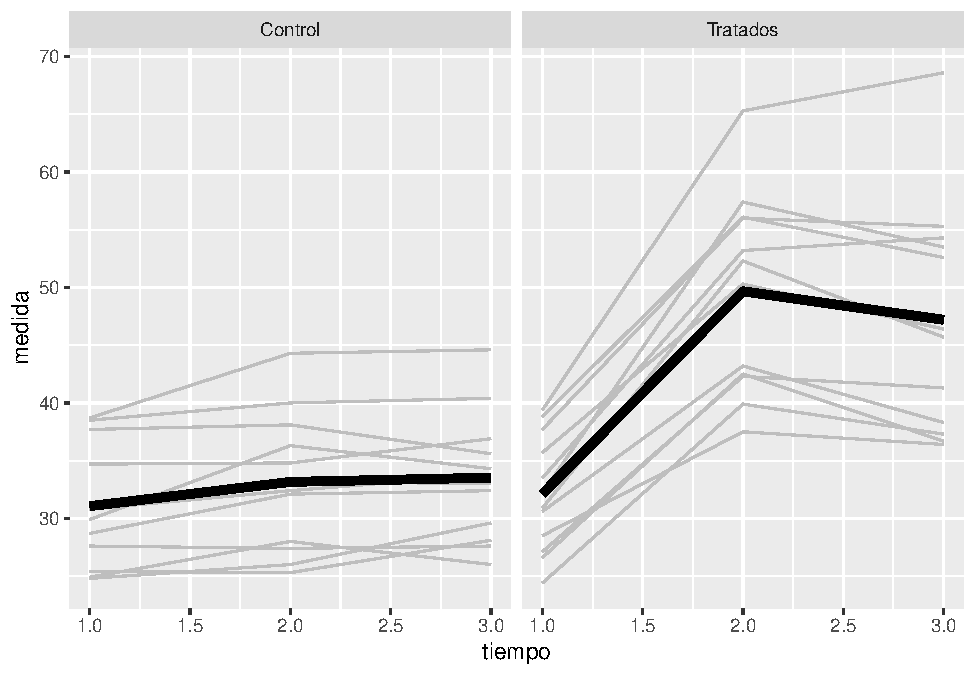
\includegraphics{fig_out/unnamed-chunk-58-1.pdf}

Para \texttt{trat=1}, la medida parece que no sube o sube muy poco. Mientras que para \texttt{trat=2} sube mucho hasta la segunda medida y se estabiliza en la tercera medida. Por lo tanto, parece que sí hay una interacción entre el tiempo y el grupo de tratamiento.

\hypertarget{suma-de-cuadrados-anova-1}{%
\subsubsection{Suma de cuadrados (ANOVA)}\label{suma-de-cuadrados-anova-1}}

Para ajustar este modelo hay que usar los datos en disposición vertical.
Como antes hay que convertir las variables \texttt{tiempo}, \texttt{indiv2} y \texttt{trat} a factor.

\begin{Shaded}
\begin{Highlighting}[]
\FunctionTok{library}\NormalTok{(ez)}

\NormalTok{datos.ez }\OtherTok{\textless{}{-}}\NormalTok{ datos}
\NormalTok{datos.ez}\SpecialCharTok{$}\NormalTok{tiempo }\OtherTok{\textless{}{-}} \FunctionTok{factor}\NormalTok{(datos.ez}\SpecialCharTok{$}\NormalTok{tiempo)}
\NormalTok{datos.ez}\SpecialCharTok{$}\NormalTok{indiv2 }\OtherTok{\textless{}{-}} \FunctionTok{factor}\NormalTok{(datos.ez}\SpecialCharTok{$}\NormalTok{indiv2)}
\NormalTok{datos.ez}\SpecialCharTok{$}\NormalTok{trat }\OtherTok{\textless{}{-}} \FunctionTok{factor}\NormalTok{(datos.ez}\SpecialCharTok{$}\NormalTok{trat)}

\FunctionTok{ezANOVA}\NormalTok{(}\AttributeTok{data=}\NormalTok{datos.ez, }
        \AttributeTok{dv=}\NormalTok{medida, }
        \AttributeTok{wid=}\NormalTok{indiv, }
        \AttributeTok{within=}\NormalTok{tiempo, }
        \AttributeTok{between=}\NormalTok{trat,}
        \AttributeTok{detailed =} \ConstantTok{TRUE}\NormalTok{)}
\end{Highlighting}
\end{Shaded}

\begin{verbatim}
$ANOVA
       Effect DFn DFd         SSn       SSd
1 (Intercept)   1  22 102808.4513 2849.9219
2        trat   1  22   1952.0835 2849.9219
3      tiempo   2  44   1397.0700  312.7422
4 trat:tiempo   2  44    811.8211  312.7422
          F            p p<.05       ges
1 793.63083 9.363797e-19     * 0.9701554
2  15.06913 8.040878e-04     * 0.3816578
3  98.27755 5.878117e-17     * 0.3063929
4  57.10794 5.921847e-13     * 0.2042582

$`Mauchly's Test for Sphericity`
       Effect         W           p p<.05
3      tiempo 0.5725954 0.002866835     *
4 trat:tiempo 0.5725954 0.002866835     *

$`Sphericity Corrections`
       Effect       GGe        p[GG] p[GG]<.05
3      tiempo 0.7005722 1.520842e-12         *
4 trat:tiempo 0.7005722 1.003472e-09         *
        HFe        p[HF] p[HF]<.05
3 0.7336894 4.932994e-13         *
4 0.7336894 4.400536e-10         *
\end{verbatim}

Vemos como se aplican las correcciones sólo en los términos ``intra sujeto'' que son \texttt{tiempo} y la interacción \texttt{trat:tiempo}, ya que el test de Mauchly es significativo (p-valor \textless{} 0.05).
Una vez aplicados las correcciones sobre los grados de libertad, los p-valores cambian aunque las conclusiones son las mismas: tanto el efecto del tiempo como su interacción con el tratamiento son significativos.

\begin{Shaded}
\begin{Highlighting}[]
\FunctionTok{ezPlot}\NormalTok{(}\AttributeTok{data=}\NormalTok{datos.ez, }
       \AttributeTok{dv=}\NormalTok{medida, }
       \AttributeTok{wid=}\NormalTok{indiv, }
       \AttributeTok{within=}\NormalTok{tiempo, }
       \AttributeTok{between=}\NormalTok{trat,}
       \AttributeTok{x=}\NormalTok{tiempo,}
       \AttributeTok{split=}\NormalTok{trat)}
\end{Highlighting}
\end{Shaded}

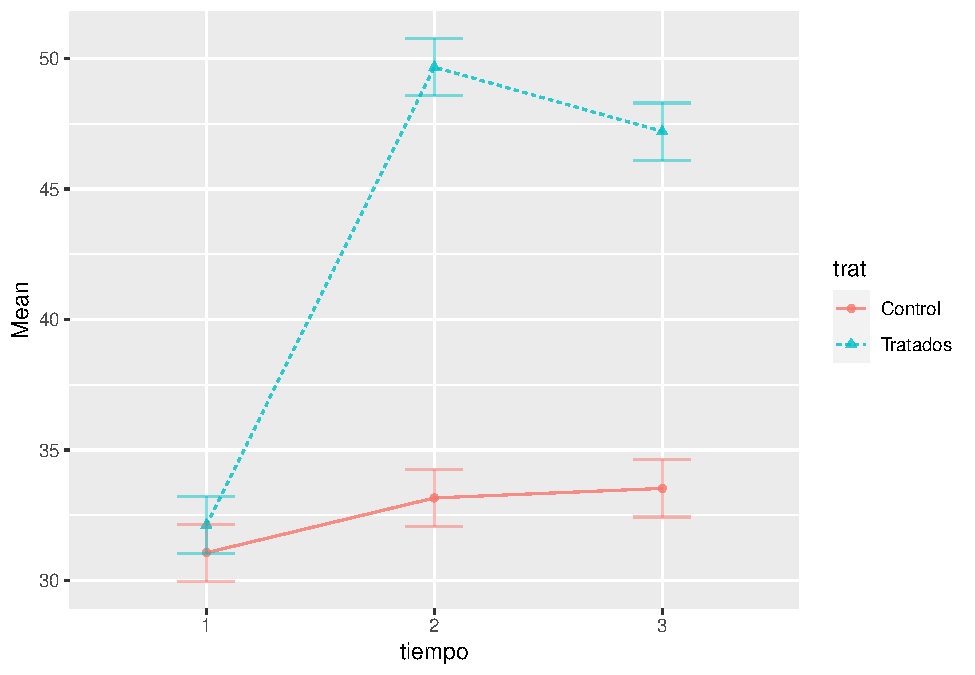
\includegraphics{fig_out/unnamed-chunk-60-1.pdf}

Las conclusiones con la tabla ANOVA corregida (tanto por GG como por HF), se ven claramente en el gráfico de interacción.

\hypertarget{modelo-de-respuesta-multivariante-manova-1}{%
\subsubsection{Modelo de respuesta multivariante (MANOVA)}\label{modelo-de-respuesta-multivariante-manova-1}}

Para analizar los datos mediante el modelo de respuesta multivariante, como antes hay que disponer los datos de forma horizontal.

\begin{Shaded}
\begin{Highlighting}[]
\NormalTok{datosh }\OtherTok{\textless{}{-}} \FunctionTok{dcast}\NormalTok{(datos, indiv }\SpecialCharTok{+}\NormalTok{ trat }\SpecialCharTok{\textasciitilde{}} \FunctionTok{paste0}\NormalTok{(}\StringTok{"medida\_"}\NormalTok{, tiempo),}
                 \AttributeTok{value.var =} \StringTok{"medida"}\NormalTok{ )}
\NormalTok{datosh}
\end{Highlighting}
\end{Shaded}

\begin{verbatim}
   indiv     trat medida_1 medida_2 medida_3
1      1  Control     34.7     34.8     36.9
2      1 Tratados     39.4     65.3     68.6
3      2  Control     38.7     44.3     44.6
4      2 Tratados     33.5     53.2     54.3
5      3  Control     28.7     32.1     32.4
6      3 Tratados     27.1     42.3     41.3
7      4  Control     30.8     32.4     33.8
8      4 Tratados     30.9     52.3     45.7
9      5  Control     29.9     36.3     34.3
10     5 Tratados     32.2     57.4     53.5
11     6  Control     27.6     27.4     27.6
12     6 Tratados     26.6     42.5     36.7
13     7  Control     24.9     28.0     26.0
14     7 Tratados     28.5     37.5     36.4
15     8  Control     37.7     38.1     35.6
16     8 Tratados     37.7     56.0     55.3
17     9  Control     31.0     33.2     33.0
18     9 Tratados     35.7     50.3     46.4
19    10  Control     25.4     25.3     28.1
20    10 Tratados     30.6     43.2     38.3
21    11  Control     24.8     26.0     29.6
22    11 Tratados     24.4     39.9     37.3
23    12  Control     38.5     40.0     40.4
24    12 Tratados     38.8     56.1     52.6
\end{verbatim}

\begin{Shaded}
\begin{Highlighting}[]
\NormalTok{respuesta }\OtherTok{\textless{}{-}} \FunctionTok{as.matrix}\NormalTok{(datosh[,}\FunctionTok{c}\NormalTok{(}\StringTok{"medida\_1"}\NormalTok{,}\StringTok{"medida\_2"}\NormalTok{,}\StringTok{"medida\_3"}\NormalTok{)])}
\NormalTok{modelo }\OtherTok{\textless{}{-}} \FunctionTok{lm}\NormalTok{(respuesta }\SpecialCharTok{\textasciitilde{}}\NormalTok{ trat, }\AttributeTok{data=}\NormalTok{datosh)}
\FunctionTok{summary}\NormalTok{(modelo)}
\end{Highlighting}
\end{Shaded}

\begin{verbatim}
Response medida_1 :

Call:
lm(formula = medida_1 ~ trat, data = datosh)

Residuals:
    Min      1Q  Median      3Q     Max 
-7.7167 -3.9667 -0.7083  4.1271  7.6417 

Coefficients:
             Estimate Std. Error t value
(Intercept)    31.058      1.476  21.048
tratTratados    1.058      2.087   0.507
             Pr(>|t|)    
(Intercept)  4.57e-16 ***
tratTratados    0.617    
---
Signif. codes:  
0 '***' 0.001 '**' 0.01 '*' 0.05 '.' 0.1 ' ' 1

Residual standard error: 5.112 on 22 degrees of freedom
Multiple R-squared:  0.01156,   Adjusted R-squared:  -0.03337 
F-statistic: 0.2572 on 1 and 22 DF,  p-value: 0.6171


Response medida_2 :

Call:
lm(formula = medida_2 ~ trat, data = datosh)

Residuals:
     Min       1Q   Median       3Q      Max 
-12.1667  -6.6396   0.3375   5.2896  15.6333 

Coefficients:
             Estimate Std. Error t value
(Intercept)    33.158      2.113  15.692
tratTratados   16.508      2.988   5.524
             Pr(>|t|)    
(Intercept)  1.98e-13 ***
tratTratados 1.50e-05 ***
---
Signif. codes:  
0 '***' 0.001 '**' 0.01 '*' 0.05 '.' 0.1 ' ' 1

Residual standard error: 7.32 on 22 degrees of freedom
Multiple R-squared:  0.5811,    Adjusted R-squared:  0.5621 
F-statistic: 30.52 on 1 and 22 DF,  p-value: 1.495e-05


Response medida_3 :

Call:
lm(formula = medida_3 ~ trat, data = datosh)

Residuals:
     Min       1Q   Median       3Q      Max 
-10.8000  -5.9063  -0.6625   5.6250  21.4000 

Coefficients:
             Estimate Std. Error t value
(Intercept)    33.525      2.310  14.511
tratTratados   13.675      3.267   4.186
             Pr(>|t|)    
(Intercept)  9.55e-13 ***
tratTratados 0.000384 ***
---
Signif. codes:  
0 '***' 0.001 '**' 0.01 '*' 0.05 '.' 0.1 ' ' 1

Residual standard error: 8.003 on 22 degrees of freedom
Multiple R-squared:  0.4433,    Adjusted R-squared:  0.418 
F-statistic: 17.52 on 1 and 22 DF,  p-value: 0.0003835
\end{verbatim}

\begin{Shaded}
\begin{Highlighting}[]
\FunctionTok{anova}\NormalTok{(modelo, }\AttributeTok{X=}\SpecialCharTok{\textasciitilde{}}\DecValTok{1}\NormalTok{)}
\end{Highlighting}
\end{Shaded}

\begin{verbatim}
Analysis of Variance Table


Contrasts orthogonal to
~1

            Df  Pillai approx F num Df den Df
(Intercept)  1 0.88537   81.102      2     21
trat         1 0.83628   53.633      2     21
Residuals   22                               
               Pr(>F)    
(Intercept) 1.326e-10 ***
trat        5.599e-09 ***
Residuals                
---
Signif. codes:  
0 '***' 0.001 '**' 0.01 '*' 0.05 '.' 0.1 ' ' 1
\end{verbatim}

Con la instrucción \texttt{summary}, contrasta si la media es diferente entre los dos grupos de tratamiento, y esto lo hace para cada momento por separado.

En la tabla ANOVA, el p-valor de término \texttt{trat} contrasta si el efecto del tiempo es el mismo para los dos tratamientos, o sea, la interacción tratamiento y tiempo, que es lo que nos interesa. Mientras que el término \texttt{(Intercept)} corresponde al efecto marginal del tiempo.

Fíjate qué pasa si no se especifica el argumento \texttt{X}:

\begin{Shaded}
\begin{Highlighting}[]
\FunctionTok{anova}\NormalTok{(modelo)}
\end{Highlighting}
\end{Shaded}

\begin{verbatim}
Analysis of Variance Table

            Df  Pillai approx F num Df den Df
(Intercept)  1 0.97752  289.829      3     20
trat         1 0.84439   36.176      3     20
Residuals   22                               
               Pr(>F)    
(Intercept) < 2.2e-16 ***
trat        2.854e-08 ***
Residuals                
---
Signif. codes:  
0 '***' 0.001 '**' 0.01 '*' 0.05 '.' 0.1 ' ' 1
\end{verbatim}

En este caso, el p-valor del tratamiento contrasta si hay diferencias entre tratamientos en alguno de los momentos (hay 3 grados de libertad). Y este contraste no es la interacción entre tratamiento y tiempo.

\hypertarget{Ejemplo3}{%
\subsection{Ejemplo 3}\label{Ejemplo3}}

En un estudio se quieren comparar el efecto de régimen de ejercicio sobre el sobrepeso. Para ello se reclutan 100 personas. A la mitad se le asigna el régimen y al resto se le hacen algunas recomendaciones (grupo control). Se mide el índice de masa corporal justo antes de empezar el estudio (momento basal), y al cabo de 1, 2 y 3 semanas. Como la edad es una variable importante para predecir el IMC también se registra.

Los datos los encontrarás en el fichero ``imc.csv''

En este ejemplo, vemos como en algunos de los individuos nos falta alguna medida en a partir de la primera semana. Por este motivo usaremos la técnica de los LMM.

\begin{Shaded}
\begin{Highlighting}[]
\NormalTok{datos }\OtherTok{\textless{}{-}} \FunctionTok{read.csv2}\NormalTok{(}\StringTok{"datos/imc.csv"}\NormalTok{)}
\end{Highlighting}
\end{Shaded}

Nos aseguramos que los datos estén ordenados por individuo y tiempo

\begin{Shaded}
\begin{Highlighting}[]
\NormalTok{datos }\OtherTok{\textless{}{-}} \FunctionTok{arrange}\NormalTok{(datos, indiv, tiempo)}
\end{Highlighting}
\end{Shaded}

Recodificamos nuestra variable tratamiento:

\begin{Shaded}
\begin{Highlighting}[]
\NormalTok{datos}\SpecialCharTok{$}\NormalTok{tx }\OtherTok{\textless{}{-}} \FunctionTok{factor}\NormalTok{(datos}\SpecialCharTok{$}\NormalTok{tx, }\DecValTok{1}\SpecialCharTok{:}\DecValTok{2}\NormalTok{, }\FunctionTok{c}\NormalTok{(}\StringTok{"Control"}\NormalTok{, }\StringTok{"Tratados"}\NormalTok{))}
\FunctionTok{summary}\NormalTok{(datos)}
\end{Highlighting}
\end{Shaded}

\begin{verbatim}
   respuesta         indiv            tiempo    
 Min.   : 9.80   Min.   :  1.00   Min.   :0.00  
 1st Qu.:27.02   1st Qu.: 25.75   1st Qu.:0.75  
 Median :30.75   Median : 50.50   Median :1.50  
 Mean   :30.46   Mean   : 50.50   Mean   :1.50  
 3rd Qu.:34.60   3rd Qu.: 75.25   3rd Qu.:2.25  
 Max.   :43.70   Max.   :100.00   Max.   :3.00  
 NA's   :50                                     
      edad              tx     
 Min.   :25.00   Control :200  
 1st Qu.:43.00   Tratados:200  
 Median :49.00                 
 Mean   :49.03                 
 3rd Qu.:57.00                 
 Max.   :69.00                 
                               
\end{verbatim}

Comprobemos si tenemos algún inviduo con datos faltantes

\begin{Shaded}
\begin{Highlighting}[]
\FunctionTok{sum}\NormalTok{(}\FunctionTok{with}\NormalTok{(datos, }\FunctionTok{tapply}\NormalTok{(}\FunctionTok{is.na}\NormalTok{(respuesta), indiv, any)))}
\end{Highlighting}
\end{Shaded}

\begin{verbatim}
[1] 42
\end{verbatim}

Como hay individuos con datos faltantes no podemos utilizar ANOVA o MANOVA y debemos usar modelos más avanzados que veremos más adelante.

\hypertarget{ejercicios}{%
\section{Ejercicios}\label{ejercicios}}

\hypertarget{ejercicio-1}{%
\subsection{Ejercicio 1}\label{ejercicio-1}}

\begin{quote}
Para estudiar las diferencias entre dos procedimientos diferentes de recuperación de pacientes de un infarto, se consideraron dos grupos experimentales en sendos hospitales, de 8 pacientes cada uno. La variable respuesta es el índice de Bartel, que varía entre 0 y 100, y que constituye una medida de la habilidad funcional con la que se valoran diferentes capacidades, de forma que valores más altos se corresponden con una mejor situación del paciente. De cada uno de los 16 pacientes se dispone de su respuesta cada semana a lo largo de 5 semanas consecutivas. Los datos se pueden encontrar en el archivo \emph{recuperainfarto.txt}. El fichero contiene la información para cada individuo en una fila, la primera columna contiene la información del hostpital y las siguiente 5 columnas corresponden al valor del índice para cada semana.

\begin{enumerate}
\def\labelenumi{\arabic{enumi}.}
\tightlist
\item
  Carga los datos en R.
\item
  Nombra a las columnas del data.frame con `c(``hospital'', ``bartel\_1'', ``bartel\_2'', ``bartel\_3''), ``bartel\_4'', ``bartel\_5'')
\item
  Añade una columna (\texttt{id}) a los datos que corresponda al identificador cada individuo (usa 1, 2, 3, \ldots{} 16).
\item
  Crea un data.frame con los datos en formato largo
\item
  Crea una figura para visualizar la evolución en la respuesta a lo largo del tiempo para cada individuo.
\item
  Crea una figura para mostrar si visualmente hay diferencias entre ambos procedimientos a lo largo del tiempo.
\item
  ¿Qué procedimiento presenta una mejor recuperación de los pacientes? ¿Es esta diferencia estadísticamente significativa?
\end{enumerate}
\end{quote}

\hypertarget{ejercicio-2}{%
\subsection{Ejercicio 2}\label{ejercicio-2}}

\begin{quote}
En un estudio sobre la agudeza visual se dispone de la respuesta de siete individuos. La respuesta en cada ojo es el retraso en milisegundos entre la emisión de una luz y la respuesta en a la misma por el cortex. Cada ojo se somete a cuatro mediciones correspondientes a cuatro instantes consecutivos. Se tienen mediciones en el ojo izquierdo y derecho. Los datos se pueden encontrar en el archivo \emph{agudezavisual.txt}

\begin{enumerate}
\def\labelenumi{\arabic{enumi}.}
\tightlist
\item
  Crea una nueva base de datos agregando la información para cada una de la medida repetida (ojo) {[}NOTA: toma la media - usa la función \texttt{aggregate} o cualquier otra que creas oportuna{]}. Usando esta nueva base de datos, contesta a las siguientes preguntas:
\item
  Crea una figura para mostrar si visualmente hay diferencias en el retraso promedio de ambos ojos a lo largo del tiempo para cada individuo.
\item
  ¿Existen diferencias entre la medición final y la basal?
\item
  ¿Existe un efecto temporal en la respuesta?
\end{enumerate}
\end{quote}

\hypertarget{ejercicio-3}{%
\subsection{Ejercicio 3}\label{ejercicio-3}}

\begin{quote}
Los datos \texttt{o2cons}, disponibles en el paquete \texttt{MANOVA.RM}, contiene medidas sobre el consumo de oxígeno de los leucocitos (``O2'') de 144 individuos, 72 de ellos asignados al grupo control (``Group=P'') y el resto al grupo de tratamiento con Verum (Group=V). Además, para cada individuo se recoge si los estafilococos (``Staphylococci'') estaban activados o no (0/1). Para cada individuo se tomaron los niveles de oxígeno de los leucocitos después de 6, 12 y 18 minutos.

\begin{enumerate}
\def\labelenumi{\arabic{enumi}.}
\tightlist
\item
  Crea otro data.frame con los datos en formato ancho
\item
  Haz una pequeña descriptiva de los datos contenidos en esta base de datos
\item
  Analiza la evolución del consumo de oxígeno del grupo de tratamiento (``Group=V'').
\item
  Crea una figura para mostrar si visualmente hay diferencias en la evolución del comsumo de O2 entre el grupo de intervención y el grupo de tratamiento.
\item
  ¿Son estas diferencias estadísticamente significativas?
\end{enumerate}

Recuerda que los datos los puedes cargar mediante la instrucción
\end{quote}

\begin{Shaded}
\begin{Highlighting}[]
\FunctionTok{library}\NormalTok{(MANOVA.RM)}
\FunctionTok{data}\NormalTok{(o2cons)}
\end{Highlighting}
\end{Shaded}

\begin{quote}
\end{quote}

\hypertarget{modelos-lineales-mixtos-lmm}{%
\chapter{Modelos Lineales Mixtos (LMM)}\label{modelos-lineales-mixtos-lmm}}

Esta técnica es la más potente para analizar datos longitudinales ya que permite introducir efectos aleatorios y especificar la estructura de correlaciones de los residuos dentro de un mismo individuo.

Además, a diferencia de las dos técnicas anteriores, permite trabajar con missings.

\hypertarget{ecuaciuxf3n}{%
\section{Ecuación}\label{ecuaciuxf3n}}

\[
y_{ij} = \beta_{0i} + \sum_{k=1}^K \beta_{ki} x_{ijk} + e_{ij}
\]

Donde \(i\) representa al individuo, \(j\) representa el momento (de uno hasta hasta el número de observaciones del individuo \(i\)),

\begin{itemize}
\item
  \(x_{ijk}\) valor de la \(k\)-ésima variable independiente del individuo \(i\) en el momento \(j\).
\item
  \(\beta_{0i} \sim N\left(\beta_0, \sigma_{\beta_0}^2\right)\) es la constante del modelo aunque en general se supone aleatoria, o sea que tiene cierta varianza entre individuos y está centrada en la contaste \(\mu\).
\item
  \(\beta_{ki} \sim N\left(\beta_k, \sigma_{\beta_k}^2\right)\): pendientes o coeficientes de las variables del modelo. Pueden ser aleatorias, o sea, variar entre individuos.
\end{itemize}

En general puede haber correlación entre la contante \(\beta_{0i}\) y las pendientes \(\beta_{ki}\).

El vector formado por la constante y por los coeficientes aleatorios, son los \textbf{efectos aleatorios} y se supone que sigue una distribución normal multivariada:

\[\vec{\beta}_i = (\beta_{0i},\beta_{1i},\ldots,\beta_{Ki})^t \sim N\left(\vec{\beta}, \Omega) \right)\]

\begin{itemize}
\tightlist
\item
  El vector formado por los errores de un individuo \(\vec{e_i} \sim N(\vec{0},\Sigma_i)\), sigue una distribuión normal multivariante con una cierta matriz de covarianzas \(\Sigma_i\) que no tiene porqué ser la misma ni del mismo tamaño para todos los individuos ya que no todos los individuos tendrán el mismo número de observaciones. \textbf{Los errores son independientes de la constante aleatoria y de los coeficientes aleatorios}.
\end{itemize}

\textbf{Observaciones}

\begin{itemize}
\item
  Para ajustar este modelo los datos se disponen de forma vertical.
\item
  El modelo LMM es muy flexible y potente. No sólo permite especificar efectos aleatorios con lo que evaluar la variabilidad de ciertos efectos o variables entre individuos sinó también la correlación residual entre las distintas medidas repetidas en un mismo individuo.
\item
  Cuando hay missings en una observación no hace falta eliminar las otras del mismo individuo, ya que cada fila aquí es una observación y no un individuo.
\item
  La esperanza de la constante y coeficientes aleatorios \(\vec{\beta}_i\) es la misma para todos los individuos, \(\vec{\beta}\), y la matriz de covarianzas, \(\Omega\), también (\textbf{homocedesticidad}).
\item
  Si un coeficiente no es aleatorio, se puede notar como \(\beta_{k'i} = \beta_{k'}\) en lugar de suponer que sigue una distribución normal. También se podría pensar que sigue una distribución ``normal'' con varianza cero.
\item
  Los \textbf{efectos fijos} son la esperanza de los efectos aleatorios (\(\beta_0, \beta_1, \ldots, \ldots, \beta_k\)). Además, cuando un coeficiente no es aleatorio (tiene varianza cero) se denomina fijo directamente.
\item
  Hay un número limitado de efectos aleatorios que se pueden incorporar en el modelo, que no puede exceder el número de medidas por individuo.
\item
  La presencia de \textbf{efectos aleatorios inducen correlación} entre medidas de un mismo individuo. Sin embargo, según que estructura de correlación sólo se puede conseguir definiendo también una estructura de correlación entre residuos no nula (no diagonal).

  \begin{itemize}
  \item
    Considerando los coeficientes del tiempo como aleatorios se induce correlación distinta según los tiempos que se toman las medidas.
  \item
    Considerando el coeficiente de una variable \textbf{no} cambiante en el tiempo se induce \textbf{heterocedesticidad} (varianza diferente) entre los individuos.
  \end{itemize}
\end{itemize}

Por ejemplo, supongamos un modelo con efecto lineal del tiempo y una covariable no cambiante del tiempo (\(x_i\)). Y tomamos la constante y el coeficiente de \(x_i\) aleatorios y ambos no correlacionados.

\[y_{ij} = \beta_{0i} + \beta_1 t_{ij} + \beta_{2i} x_i\]

Luego la varianza de \(y_{ij}\) es \(\sigma_{\beta_{0}}^2 + \sigma_{2i}^2 x_i^2\). Si \(x_i\) vale 0 para el grupo placebo y 1 para los tratados, entonces la varianza del grupo placebo será \(\sigma_{\beta_{0}}^2\) y para los tratados \(\sigma_{\beta_{0}}^2 + \sigma_{\beta_{2}}^2\)

\begin{itemize}
\tightlist
\item
  A diferencia de las técnicas de sumas de cuadrados y de respuesta multivariante, en que la variable \textbf{tiempo} se trata como a un \textbf{factor}, con los LMM se tratar también como \textbf{variable continua}.
\end{itemize}

\hypertarget{casos-particulares}{%
\section{Casos particulares}\label{casos-particulares}}

\hypertarget{modelo-con-constante-aleatoria}{%
\subsection{Modelo con constante aleatoria}\label{modelo-con-constante-aleatoria}}

\[y_{ij} = \beta_{0i} + \beta_{1} t_{ij} + e_{ij}\]

Donde \(\beta_{0i} \sim N(\beta_0, \sigma_{\beta_0})\), y \(\beta_1\) es el coeficiente fijo del tiempo. En este caso se supone que el tiempo tiene un efecto lineal.

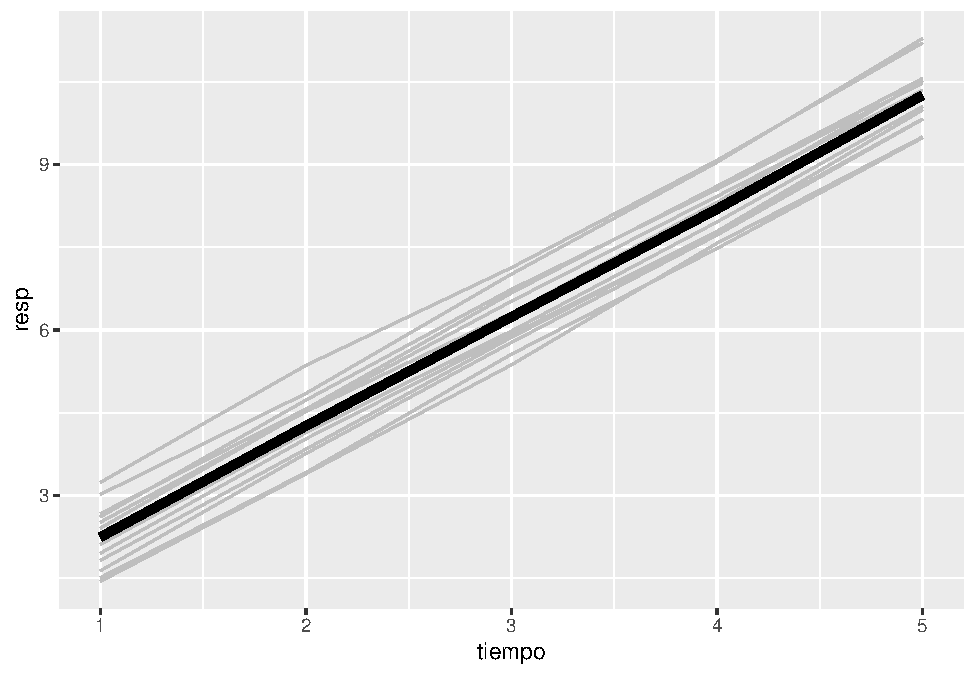
\includegraphics{fig_out/unnamed-chunk-69-1.pdf}

Podríamos añadir un término cuadrático, cúbico, etc. si el efecto no fuera lineal y añadiéramos un término cuadrático:

\[y_{ij} = \beta_{0i} + \beta_{1} t_{ij} + \beta_{2} t_{ij}^2 + e_{ij}\]
en este caso, \(x_{ij1}=t_{ij}\) y \(x_{ij2}=t_{ij}^2\).

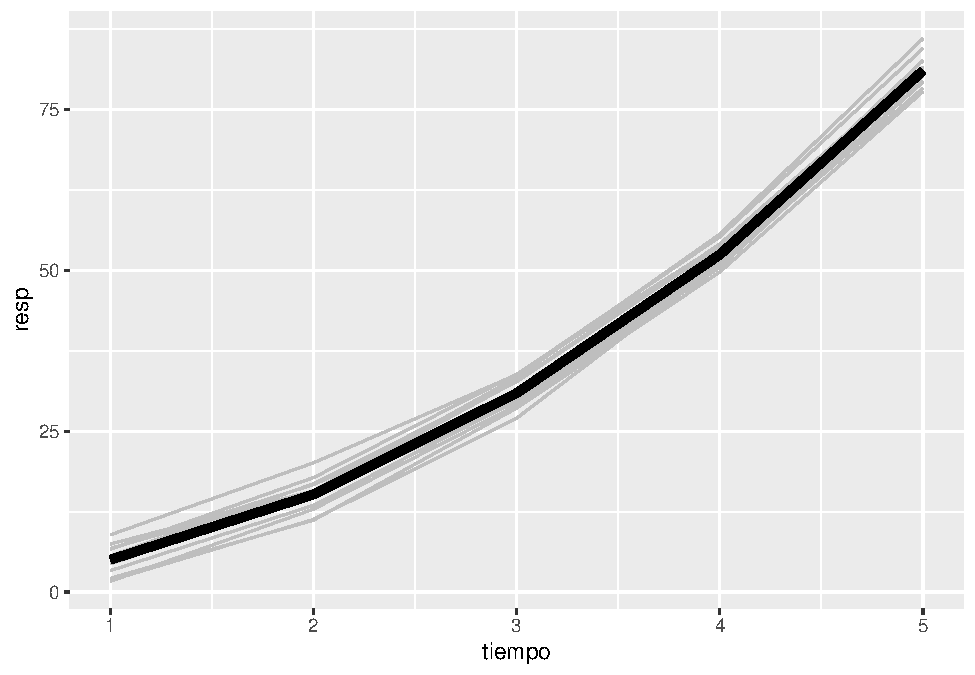
\includegraphics{fig_out/unnamed-chunk-70-1.pdf}

\textbf{Correlacion entre observaciones}

Si los errores son independientes, las observaciones de la variable respuesta de un mismo individuo están correlacionadas. Y esta correlación es constante: no depende de la distancia entre las medidas.

\[\text{corr}(y_{i1},y_{i2}) = \text{corr}(y_{i1},y_{i3}) = \ldots = \frac{\sigma_{\beta_{0}}^2}{\sigma_{e}^2}\]

A esta correlación también se la conoce como \textbf{coeficiente de correlación intraclase (ICC)}

\hypertarget{modelo-con-pendiente-y-constante-aleatoria}{%
\subsubsection{Modelo con pendiente y constante aleatoria}\label{modelo-con-pendiente-y-constante-aleatoria}}

\[y_{ij} = \beta_{0i} + \beta_{1i} t_{ij} + e_{ij}\]

\(\vec{\beta}_i = (\beta_{0i}, \beta_{1i})^t \sim N\left((\beta_0,\beta_1)^t, \Omega\right)\), donde

\[\Omega= 
\begin{pmatrix}
\sigma_{\beta_0}^2 & \sigma_{\beta_0,\beta_1} \\
\sigma_{\beta_0,\beta_1} & \sigma_{\beta_1}^2
\end{pmatrix}
\]

El término \(\sigma_{\beta_0,\beta_1}\) es la covarianza entre la constante y la pendiente. Ésta en general puede no ser cero.

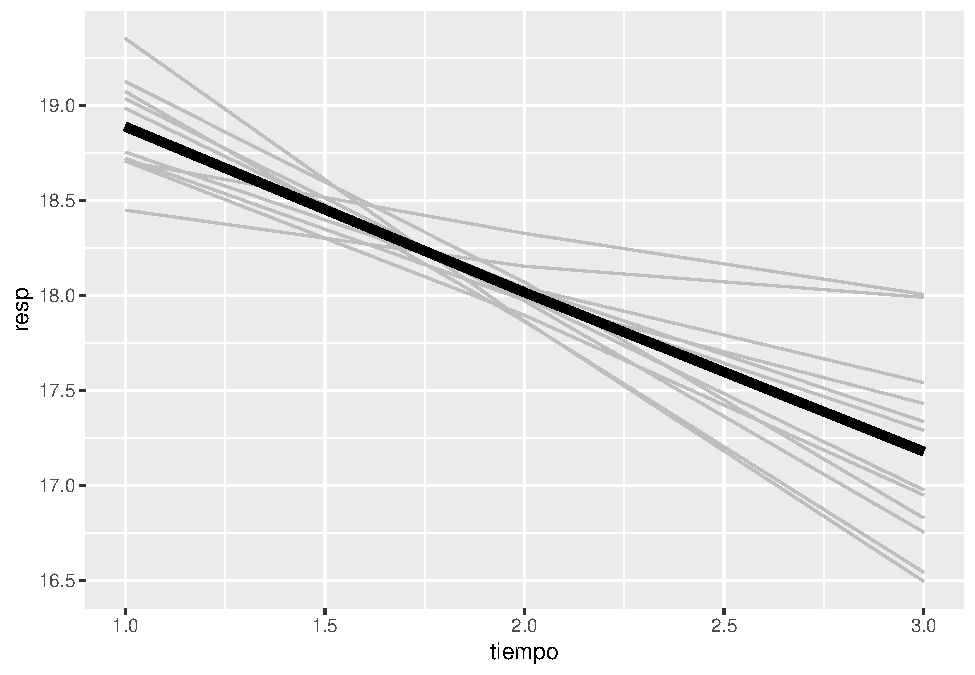
\includegraphics{fig_out/unnamed-chunk-71-1.pdf}

En este gráfico se observa primero que las pendientes son diferentes entre los individuos. Y además, que los individuos que empiezan de más arriba bajan más rápido y viceversa. Así pues, la correlación entre la constante y la pendiente es negativa.

\textbf{Correlacion entre observaciones}

En el modelo con constante y pendientes aleatorios, si asumimos que los errores son independientes, las observaciones de la variable respuesta de un mismo individuo están correlacionadas. Y esta correlación depende de los momentos:

\[\text{corr}(y_{i1},y_{i2}) = \frac{\sigma_{\beta_{0}}^2+\sigma_{\beta_{1i}^2 \cdot t_1 \cdot t_2}}{\sqrt{\sigma_{\beta_{0}}^2+\sigma_{\beta_{1}}^2 \cdot t_1^2 + \sigma_e^2}\sqrt{\sigma_{\beta_{0}}^2+\sigma_{\beta_{1}}^2 \cdot t_2^2 + \sigma_e^2}}\]

Por lo tanto depende tanto de \(t_1\) como de \(t_2\) y no sólo de la distancia entre las medidas.

Si lo comparamos con el AR(1):

Ejemplo con \(t_1=1\), \(\sigma_{\beta_{0}}^2=0.5^2\), \(\sigma_{\beta_{1}}^2=0.3^2\) y \(\sigma_{e}^2=0.1^2\), con \(t_1=1\)

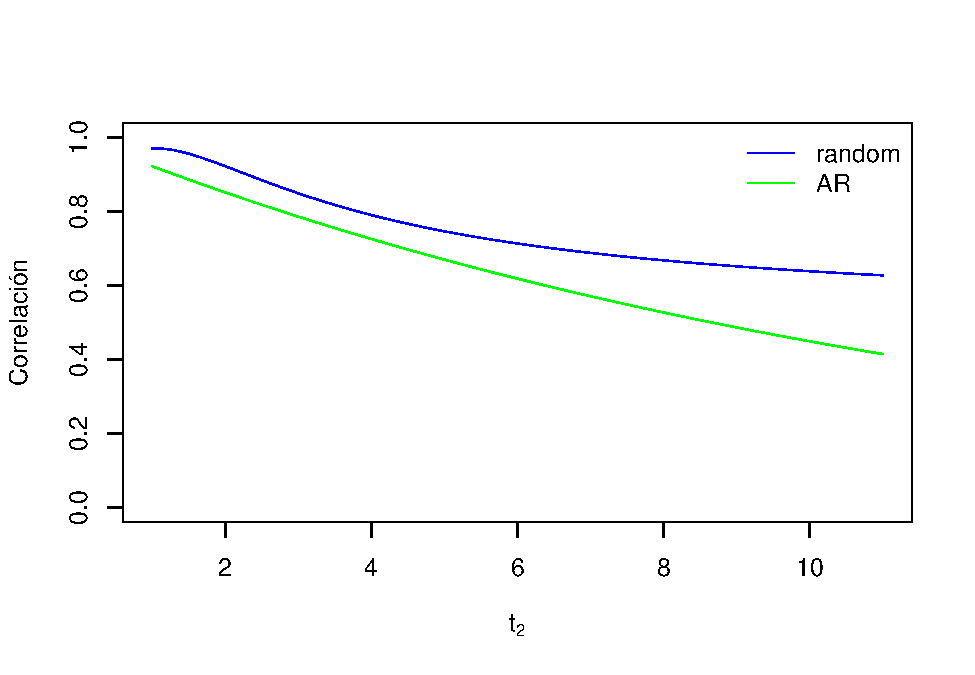
\includegraphics{fig_out/unnamed-chunk-72-1.pdf}

En este ejemplo, vemos como especificando el AR y la pendiente fija, la correlación entre observaciones baja más rápidamente a medida que las observaciones se alejan (\(t_2\)) que lo que se consigue especificando la pendiente aleatoria y los errores incorrelacionados.

\hypertarget{simplificaciuxf3n-del-modelo}{%
\section{Simplificación del modelo}\label{simplificaciuxf3n-del-modelo}}

Empezaremos con el modelo más general, o sea, sin asumir independencia de los residuos, con efectos aleatorios (todos los que se admitan) correlacionados.

En cuanto a los efectos fijos, se incluyrán también los máximos que se puedan, interacciones si es pertinente, terminos cuadráticos (cúbicos), \ldots{}

A partir de aquí se simplificará el modelo en el siguiente orden:

\hypertarget{significaciuxf3n-de-los-efectos-aleatorios}{%
\subsection{Significación de los efectos aleatorios}\label{significaciuxf3n-de-los-efectos-aleatorios}}

La hipótesis nula para contrastar los factores de efectos aleatorios es que su varianza es igual a cero. Por ejemplo para la constante aleatoria:

\[\left\{\begin{array}{l}
\text{H}_0: \sigma_{\beta_0}^2 = 0 \\
\text{H}_1: \sigma_{\beta_0}^2 > 0
\end{array}\right.
\]

Hay diferentes técnicas estadísticas para contrastar estos tests, pero no son estándard. El problema es que la varianza de una distribución normal no puede ser cero, por lo tanto la hipótesis nula está fuera del espacio parametrico (``beyond boundary''). Existen, pero, algunas herramientas en R que lo realizan mediante técnicas de remuestreo (``bootstrap''). Éstas son complejas desde el punto de visto teórico y no se explicarán en este curso (véase el paquete de R \texttt{pbkrtest} \citet{pbkrtest2014}).
Otra alternativa es usar índices como el AIC o BIC (cuanto más bajo mejor), que proporciona la función \texttt{anova} en la comparación de dos modelos: uno considerando el coeficiente como aleatorio (\(\beta_{ik}\)) el otro considerando el coeficiente como fijo (\(\beta_{k}\)).

\hypertarget{elecciuxf3n-matriz-covarianzas-de-los-efectos-aleatorios}{%
\subsection{Elección matriz covarianzas de los efectos aleatorios}\label{elecciuxf3n-matriz-covarianzas-de-los-efectos-aleatorios}}

Si en el paso anterior, hay más de un efecto aleatorio significativo, seguidamente hay que contrastar si la correlación entre ellos es cero o no. Es decir, H\(_0\) postula que la matriz \(\Omega\) es diagonal, mientras que la H\(_1\) se asume que las correlaciones pueden ser no nulas.

\[\left\{\begin{array}{l}
\text{H}_0: \Omega= 
\begin{pmatrix}
\sigma_{\beta_0}^2 & 0 \\
0 & \sigma_{\beta_1}^2
\end{pmatrix}\\
\text{H}_1: \Omega= 
\begin{pmatrix}
\sigma_{\beta_0}^2 & \sigma_{\beta_0\beta_1} \\
\sigma_{\beta_0\beta_1} & \sigma_{\beta_1}^2
\end{pmatrix}
\end{array}\right.
\]

Como la matriz diagonal es un caso particular de la matriz general, en que las correlaciones son cero se puede aplicar el test de razón de verosimilitudes.

\hypertarget{estructura-de-correlaciuxf3n-de-los-errores}{%
\subsection{Estructura de correlación de los errores}\label{estructura-de-correlaciuxf3n-de-los-errores}}

Mediante el \textbf{test de razón de verosimilitudes (LRT)}, se comparan las verosimilitudes de dos modelos.

Hay que ajustar el modelo mediante el criterio de máxima verosimilutud.

\textbf{Los modelos tienen que estar anidados}: la matriz de covarianzas de los errores de un modelo se pueda expresar como un caso particular de la del otro modelo. Por ejemplo, la matriz sin estructura sería la más general de todas, y la matriz de simetría compuesta sería un caso particular en que todas las correlación son iguales.
No están anidadas las matrices con estructura MA(1) y una AR(1).

La simetría compuesta es un caso particular de matriz sin estructura.

\[
\begin{pmatrix}
1 &  \rho_{12} & \rho_{13} \\
\rho_{12} & 1 & \rho_{23} \\
\rho_{13} & \rho_{23} & 1 \\
\end{pmatrix}
\Rightarrow \color{blue}{(\rho_{12}=\rho_{13}=\rho_{23} =\rho)} \Rightarrow
\begin{pmatrix}
1 &  \rho & \rho \\
\rho & 1 & \rho \\
\rho & \rho & 1 \\
\end{pmatrix}
\]

La matriz que supone independencia entre los residuos es un caso particular de matriz de simetría compuesta.

\[
\begin{pmatrix}
1 &  \rho & \rho \\
\rho & 1 & \rho \\
\rho & \rho & 1 \\
\end{pmatrix}
\Rightarrow \color{blue}{(\rho=0)} \Rightarrow
\begin{pmatrix}
1 &  0 & 0 \\
0 & 1 & 0 \\
0 & 0 & 1 \\
\end{pmatrix}
\]

Pero no se puede pasar de una AR(1) a una MA(1) ni viceversa. En este caso el test LRT no es válido pero sí el criterio AIC o BIC.

\[
\begin{pmatrix}
1 &  \rho & \rho^2 \\
\rho & 1 & \rho \\
\rho^2 & \rho & 1 \\
\end{pmatrix}
\Rightarrow \color{blue}{(????)} \Rightarrow
\begin{pmatrix}
1 & \frac{\theta}{1+\theta^2} & 0 \\
\frac{\theta}{1+\theta^2} & 1 & \frac{\theta}{1+\theta^2} \\
0 & \frac{\theta}{1+\theta^2} & 1 \\
\end{pmatrix}
\]

Una matriz AR(p') está anidada a AR(p) si p' \textless{} p, o sea un AR de orden menor está anidado a una de orden mayor, y por lo tanto, se puede aplicar un LRT para decidir el valor de p.~Por ejemplo, un AR de orden 3 se especificaría como \texttt{correlation\ =\ corARMA(p=3,\ q=0)}. Lo mismo sucede para decidir el orden de una MA. Por ejemplo, para una MA de orden 4, \texttt{correlation\ =\ corARMA(p=0,\ q=4)}.

\textbf{Heterocedesticidad}:

La heterocedesticidad se produce cuando los parámetros de la matriz de covarianzas \(\Sigma\) dependen de variables. Por ejemplo, del sexo o de la edad, etc, o de una combinación lineal de las variables (valor esperado).

Por ejemplo, que la varianza sea distinta según el sexo, mientras que la correlación sea la misma:

para hombres

\[ 
\Sigma_{\text{H}} = \sigma_{\text{H}}^2
\begin{pmatrix}
1 &  \rho & \rho^2 \\
\rho & 1 & \rho \\
\rho^2 & \rho & 1 \\
\end{pmatrix}
\],

y para las mujeres

\[ 
\Sigma_{\text{M}} = \sigma_{\text{M}}^2
\begin{pmatrix}
1 &  \rho & \rho^2 \\
\rho & 1 & \rho \\
\rho^2 & \rho & 1 \\
\end{pmatrix}
\]

También podríamos definir las varianzas (diagonal de \(\Sigma\)), en función del tiempo.

Veremos como es posible modelizar diferentes varianzas distintas entre grupos de individuos con la función \texttt{lme} de R que se describirá en esta sección.

\hypertarget{efectos-fijos}{%
\subsection{Efectos fijos}\label{efectos-fijos}}

Una vez escogida la estructura de covarianzas de los efectos aleatorios, de los errores, y qué efectos son aleatorios (contraste sobre sus varianzas), vamos a contrastar la significación de los efectos fijos:

Para ello, se puede usar el test de Wald para testar un único parámetro:

\[
\left\{\begin{array}{l}
\text{H}_0: \beta_1 = 0\\
\text{H}_1: \beta_1 \neq 0
\end{array}\right.
\]

o LRT para testar más de un parámetro a la vez, por ejemplo las dummies de un factor de más de dos categorías:

\[
\left\{\begin{array}{l}
\text{H}_0: \beta_1 = \beta_2 = 0\\
\text{H}_1: \text{alguno diferente de 0}
\end{array}\right.
\]

\hypertarget{validaciuxf3n-del-modelo}{%
\section{Validación del modelo}\label{validaciuxf3n-del-modelo}}

Una vez simplificado y seleccionado el modelo, hay que validarlo.

De todas las premisas a comprobar en este curso nos limitaremos a las asumciones sobre los \textbf{residuos}.

Para ellos se realizarán dos gráficos:

\begin{itemize}
\item
  \textbf{Residuos estandarizados vs valores predichos:} en este gráficos debería aparecer una nube de puntos
  uniformemente distribuida sin ninguna tendencia. Ésto nos indicaría que no nos hemos dejado ninguna variable, o ningún término cuadrático o cúbico del tiempo.
\item
  \textbf{QQ-plot:} éste gráfico está pensado para comprobar la normalidad. Si los puntos se encuentran alrededor de la diagonal sin seguir ningún patrón, dará evidencia de que los residuos siguen una distribución normal
\end{itemize}

Hay otras premisas que se deberían comprobar, como por ejemplo la normalidad de los efectos aleatorios. Pero, por su complejidad, no se verá en este curso.

La valicación de los \textbf{efectos aleatorios} es más compleja. Una posibilidad ``naive'' es considerar que sus estimaciones siguen una distribución normal y que su distribución no depende de ninguna covariable a nivel de individuo. Veremos como las funciones de R para estimar los LMM proporcionan las estimaciones de los efectos aleatorios (``Empirical Bayes Estimates''). Aunque los efectos aleatorios se suponen normalmente distribuidos, los ``Empirical Bayes Estimates'' no tienen porqué.

\hypertarget{predicciones}{%
\section{Predicciones}\label{predicciones}}

\hypertarget{efectos-marginales}{%
\subsection{Efectos marginales}\label{efectos-marginales}}

Los efectos marginales representan el valor esperado de la variable respuesta. Para calcularlos hay que especificar los valores de las variables predictoras (condicionar):

\[E(Y_{ij} | x_{ij1},\ldots,x_{ijK}) = \beta_0 + \sum_{k=i}^K \beta_k x_{ijk}\]

Una vez ajustado el modelo con los datos de la muestra, se estiman los valores de los parámetros para estimar los efectos marginales o predicciones.

\[\hat{E}(Y_{ij} | x_{ij1},\ldots,x_{ijK}) = \hat{\beta}_0 + \sum_{k=i}^K \hat{\beta}_k x_{ijk}\]

\hypertarget{estimaciuxf3n-de-los-efectos-aleatorios}{%
\subsection{Estimación de los efectos aleatorios}\label{estimaciuxf3n-de-los-efectos-aleatorios}}

También podemos condicionar al individuo:

\[\hat{E}(Y_{ij} | x_{ij1},\ldots,x_{ijK}, i) = \hat{\beta}_{0i} + \sum_{k=i}^K \hat{\beta}_{ki} x_{ijk}\]

Donde \(\hat{\beta}_{0i}\), \(\hat{\beta}_{ki}\) son los ``Empirical Bayes Estimates''.

\hypertarget{funciuxf3n-lme}{%
\section{\texorpdfstring{Función \texttt{lme}}{Función lme}}\label{funciuxf3n-lme}}

Para ajustar los modelos lineales mixtos usaremos la función \textbf{\texttt{lme}} del paquete \textbf{\texttt{nlme}} \citep{R-nlme}.
Esta función permite incorporar efectos aleatorios, así como especificar la estructura de la matriz de correlaciones de los residuos.

El método se basa en el \textbf{criterio de máxima verosimilidud} (``Maximum Likelihood'' - ML), que busca el valor de los parámetros que maximizan la función de verosimilitud. Generalmente, la solución no es una fórmula cerrada y se necesitan métodos iterativos numéricos para encontrar el óptimo. También se calculan mediante métodos numéricos la primera y segunda derivada para acelerar el proceso de estimación y para obtener los errores estándard de las estimaciones.

Para usar la función \texttt{lme}, los datos deben estar en formato horizontal. No hace falta que haya el mismo número de medidas para cada individuo, ni que las medidas se hayan producido en los mismos tiempos.

\begin{Shaded}
\begin{Highlighting}[]
\FunctionTok{library}\NormalTok{(nlme)}
\end{Highlighting}
\end{Shaded}

\begin{Shaded}
\begin{Highlighting}[]
\NormalTok{?lme}
\end{Highlighting}
\end{Shaded}

Los \textbf{argumentos} más importantes de la función \texttt{lme}

\begin{itemize}
\tightlist
\item
  \textbf{\texttt{fixed}}: Fórmula de la forma
\end{itemize}

\begin{verbatim}
respuesta ~ var1 + var2 + var3
\end{verbatim}

La constante se presupone que está y no hace falta escribir \texttt{1+}.
La sintaxis es la misma que para el ``formula environment'' de otras funciones estándard como \texttt{lm} para regresión lineal ordinaria (los términos van separados con \texttt{+}, las interacciones se especifican con \texttt{:}, etc.).
A la izquierda de \texttt{\textasciitilde{}} se especifica la variable respuesta.

\begin{itemize}
\tightlist
\item
  \textbf{\texttt{random}}: fórmula de la forma
\end{itemize}

\begin{verbatim}
 ~ var1 + var2 + ... + varK | indiv
\end{verbatim}

sin ninguna variable a la izquierda de \texttt{\textasciitilde{}}, donde \texttt{indiv} es la variable sujeto y \texttt{var1}, \texttt{var2}, \ldots{} \texttt{varK} son las variables con coeficiente aleatorio.
Por defecto se supone que la constante está incluida.

Si se desea que la constante no sea aleatoria
\texttt{\textasciitilde{}\ var1\ +\ ...\ +\ varK\ -\ 1\ \textbar{}\ indiv}.

Si sólo la constante es aleatoria
\texttt{\textasciitilde{}\ 1\ \textbar{}\ indiv}

Para especificar que la matriz \(\Omega\) es diagonal se usa la función \texttt{pdDiag}

\texttt{list(indiv\ =\ pdDiag(\ \textasciitilde{}\ var1\ +\ var2\ +\ ...\ +\ varK))}

Si los individuos estuvieran anidados en clústers aleatorios:
\texttt{\textasciitilde{}\ var1+..\textbar{}\ clusters\ /\ indiv}

\begin{itemize}
\item
  \textbf{correlation}: Para especificar la forma de la matriz de covarianzas de los residuos \(\Sigma_i\). Para más estructuras: \texttt{?corClasses}

  \begin{itemize}
  \item
    Residuos independientes (valor por defecto): \texttt{NULL}
  \item
    Simetría compuesta: \texttt{corCompSymm()}
  \item
    AR(1): \texttt{corAR1()}
  \item
    ARMA(p,q): \texttt{corARMA(p,q)}
  \item
    \(\phi^{|t_i-t_j|}\): \texttt{corCAR1(form\ =\ \textasciitilde{}\ tiempo\ \textbar{}\ indiv)}
  \item
    Sin estructura \textbar{} \texttt{corSymm()}
  \end{itemize}
\end{itemize}

Para \texttt{corCAR1}, \(\phi\) es la correlación entre dos medidas a distancia de una unidad de tiempo.

\textbf{Importante!:} para \texttt{corCompSymm}, \texttt{corAR1}, \texttt{corARMA} o \texttt{corSymm}, las medidas tienen que estar ordenadas dentro de cada individuo. Si no, hay que especificar la variable momento,

\begin{verbatim}
corAR1(form = ~ tiempo | indiv)
\end{verbatim}

\begin{itemize}
\item
  \textbf{weights}: Este argumento modeliza la varianza, \(\sigma^2\) según variables. Por defecto, \texttt{NULL} que supone que la matriz de covarianzas es la misma para todos los individuos. En lugar de una variable, puede ser el valor predicho, \texttt{varFixed(fitted(.))}. Para ver más \texttt{?varClasses}.

  \begin{itemize}
  \item
    \texttt{varPower()}: \(\sigma^2(x) = |x|^{2*\theta}\)
  \item
    \texttt{varFixed()}: \(\sigma^2(x) = |x|\)
  \item
    \texttt{varConstPower()} \(\sigma^2(x) = (\theta_1 + |x|^{\theta_2})^2\)
  \end{itemize}
\end{itemize}

\begin{itemize}
\item
  \textbf{method}: Método usado para estimar los parámetros (ML o REML). Para usar el LRT, o calcular los índices AIC o BIC se usa el método ML. La función \texttt{anova} que compara dos modelos por LRT, reajusta los modelos automàticamente bajo el método ML si han sido estimados con REML.

  \begin{itemize}
  \item
    REML (``REstricted Maximum Likelihood''): método por defecto y que proporciona estimaciones no sesgadas de los parámetros.
  \item
    ML (``Maximum Likelihood''): proporciona estimaciones de los parámetros sesgados.
  \end{itemize}
\end{itemize}

\hypertarget{ejemplos-2}{%
\section{Ejemplos}\label{ejemplos-2}}

\hypertarget{ejemplo-1}{%
\subsection{Ejemplo 1}\label{ejemplo-1}}

Analicemos de nuevo el primer ejemplo que vimos en el \protect\hyperlink{Ejemplo1}{anterior tema} y que están disponibles en la base de datos ``Ejemplo\_1W.csv''. Esta fichero contiene los datos de un diseño con 12 individuos en los que se toman los niveles en sangre de un cierto parámetro lipídico. Para cada invidivuo se miden los niveles a 1, 2 y 3 horas.

Recordemos que los datos se pueden cargar en R mediante

\begin{Shaded}
\begin{Highlighting}[]
\NormalTok{datos }\OtherTok{\textless{}{-}} \FunctionTok{read.csv2}\NormalTok{(}\StringTok{"datos/Ejemplo\_1W.csv"}\NormalTok{)}
\end{Highlighting}
\end{Shaded}

Ordenamos por individuo y dentro por tiempo dentro de individuo

\begin{Shaded}
\begin{Highlighting}[]
\FunctionTok{library}\NormalTok{(dplyr)}
\NormalTok{datos }\OtherTok{\textless{}{-}} \FunctionTok{arrange}\NormalTok{(datos, indiv, tiempo)}
\end{Highlighting}
\end{Shaded}

Primero, ajustamos el modelo más complejo con constante y pendiente aleatoria, y añadimos el tiempo al cuadrado ya que vemos por el gráfico que la tendencia no es lineal.

\begin{Shaded}
\begin{Highlighting}[]
\NormalTok{modelo }\OtherTok{\textless{}{-}} \FunctionTok{lme}\NormalTok{(}\AttributeTok{fixed =}\NormalTok{ medida }\SpecialCharTok{\textasciitilde{}} \FunctionTok{poly}\NormalTok{(tiempo, }\DecValTok{2}\NormalTok{), }
              \AttributeTok{data=}\NormalTok{datos,}
              \AttributeTok{random =} \SpecialCharTok{\textasciitilde{}} \FunctionTok{poly}\NormalTok{(tiempo, }\DecValTok{2}\NormalTok{) }\SpecialCharTok{|}\NormalTok{ indiv,}
              \AttributeTok{correlation =} \FunctionTok{corAR1}\NormalTok{(}\AttributeTok{form =} \SpecialCharTok{\textasciitilde{}}\NormalTok{ tiempo }\SpecialCharTok{|}\NormalTok{ indiv)}
\NormalTok{              )}
\NormalTok{modelo}\SpecialCharTok{$}\NormalTok{modelStruct}\SpecialCharTok{$}\NormalTok{corStruct}
\end{Highlighting}
\end{Shaded}

\begin{verbatim}
Correlation structure of class corAR1 representing
         Phi 
0.0001428372 
\end{verbatim}

\begin{Shaded}
\begin{Highlighting}[]
\FunctionTok{summary}\NormalTok{(modelo)}
\end{Highlighting}
\end{Shaded}

\begin{verbatim}
Linear mixed-effects model fit by REML
  Data: datos 
       AIC      BIC    logLik
  208.6888 225.1504 -93.34439

Random effects:
 Formula: ~poly(tiempo, 2) | indiv
 Structure: General positive-definite, Log-Cholesky parametrization
                 StdDev    Corr         
(Intercept)       7.526056 (Intr) p(,2)1
poly(tiempo, 2)1 14.559990  0.881       
poly(tiempo, 2)2  5.178443 -0.663 -0.729
Residual          1.441564              

Correlation Structure: AR(1)
 Formula: ~tiempo | indiv 
 Parameter estimate(s):
         Phi 
0.0001428372 
Fixed effects:  medida ~ poly(tiempo, 2) 
                     Value Std.Error DF
(Intercept)       42.99444  2.185832 22
poly(tiempo, 2)1  36.94647  4.443447 22
poly(tiempo, 2)2 -28.30784  2.076632 22
                    t-value p-value
(Intercept)       19.669598       0
poly(tiempo, 2)1   8.314823       0
poly(tiempo, 2)2 -13.631610       0
 Correlation: 
                 (Intr) p(,2)1
poly(tiempo, 2)1  0.828       
poly(tiempo, 2)2 -0.475 -0.497

Standardized Within-Group Residuals:
       Min         Q1        Med         Q3 
-1.0450552 -0.4346930 -0.1931843  0.5001057 
       Max 
 1.1924184 

Number of Observations: 36
Number of Groups: 12 
\end{verbatim}

\begin{itemize}
\tightlist
\item
  Valor esperado de la constante y coeficientes, \(\beta_0, \ldots, \beta_K\). También se conoce como los coeficientes fijos. Para obtener la tabla de sus estimaciones y los p-valores:
\end{itemize}

\begin{Shaded}
\begin{Highlighting}[]
\FunctionTok{coef}\NormalTok{(}\FunctionTok{summary}\NormalTok{(modelo))}
\end{Highlighting}
\end{Shaded}

\begin{verbatim}
                     Value Std.Error DF
(Intercept)       42.99444  2.185832 22
poly(tiempo, 2)1  36.94647  4.443447 22
poly(tiempo, 2)2 -28.30784  2.076632 22
                    t-value      p-value
(Intercept)       19.669598 1.886788e-15
poly(tiempo, 2)1   8.314823 3.092000e-08
poly(tiempo, 2)2 -13.631610 3.311649e-12
\end{verbatim}

\begin{itemize}
\tightlist
\item
  Estimación de los efectos aleatorios, \(\color{green}{(\beta_{0i}^{*},\beta_{1i}^{*},\beta_{2i}^{*})}\)
\end{itemize}

\begin{Shaded}
\begin{Highlighting}[]
\FunctionTok{ranef}\NormalTok{(modelo)}
\end{Highlighting}
\end{Shaded}

\begin{verbatim}
    (Intercept) poly(tiempo, 2)1
1  14.730441065       30.8722315
2   4.054046210       11.0739532
3  -5.907126225       -5.2717958
4   0.001779692        0.6665792
5   4.796479128       13.7400443
6  -7.601895827      -11.9016785
7  -8.829202865      -17.6630563
8   6.499328908        7.4984525
9   0.924045128       -6.5624802
10 -5.693831230      -15.1669218
11 -8.860625561       -8.7246544
12  5.886561577        1.4393264
   poly(tiempo, 2)2
1        -6.5833764
2        -1.2028619
3         2.8619041
4        -3.8718583
5        -6.6013406
6         1.3545235
7         7.7680601
8        -0.9466624
9         1.6842059
10        3.7578624
11        2.6200805
12       -0.8405368
\end{verbatim}

Hay una fila para cada individuo.

La función \texttt{ranef} retorna \(\hat{\theta}_{ki}\), donde \(\beta_{ki} = \beta_k + \theta_{ki}\). Así pues, \(\theta_{ki} \sim N\left(0,\sigma_{\beta_{k}}^2\right)\) se pueden interpretar como los \textbf{``efectos aleatorios centrados''} tal y como se ha escrito la ecuación del modelo.

\begin{itemize}
\tightlist
\item
  Matriz de covarianzas de la constante y coeficientes aleatorios, \(\Omega\):
\end{itemize}

\begin{Shaded}
\begin{Highlighting}[]
\FunctionTok{getVarCov}\NormalTok{(modelo)}
\end{Highlighting}
\end{Shaded}

\begin{verbatim}
Random effects variance covariance matrix
                 (Intercept) poly(tiempo, 2)1
(Intercept)           56.642           96.553
poly(tiempo, 2)1      96.553          211.990
poly(tiempo, 2)2     -25.856          -54.998
                 poly(tiempo, 2)2
(Intercept)               -25.856
poly(tiempo, 2)1          -54.998
poly(tiempo, 2)2           26.816
  Standard Deviations: 7.5261 14.56 5.1784 
\end{verbatim}

\begin{itemize}
\tightlist
\item
  Matriz de correlaciones de los residuos, \(\Sigma_i\)
\end{itemize}

\begin{Shaded}
\begin{Highlighting}[]
\NormalTok{modelo}\SpecialCharTok{$}\NormalTok{modelStruct}\SpecialCharTok{$}\NormalTok{corStruct}
\end{Highlighting}
\end{Shaded}

\begin{verbatim}
Correlation structure of class corAR1 representing
         Phi 
0.0001428372 
\end{verbatim}

Podemos especificar que la correlación entre efectos aleatorios sea cero con la función \texttt{pdDiag} en el argumento \texttt{random}:

\begin{Shaded}
\begin{Highlighting}[]
\NormalTok{modelo2 }\OtherTok{\textless{}{-}} \FunctionTok{lme}\NormalTok{(}\AttributeTok{fixed =}\NormalTok{ medida }\SpecialCharTok{\textasciitilde{}} \FunctionTok{poly}\NormalTok{(tiempo, }\DecValTok{2}\NormalTok{), }
              \AttributeTok{data=}\NormalTok{datos,}
              \AttributeTok{random =} \FunctionTok{list}\NormalTok{(}\AttributeTok{indiv=}\FunctionTok{pdDiag}\NormalTok{(}\SpecialCharTok{\textasciitilde{}} \FunctionTok{poly}\NormalTok{(tiempo, }\DecValTok{2}\NormalTok{))),}
              \AttributeTok{correlation =} \FunctionTok{corAR1}\NormalTok{()}
\NormalTok{              )}
\FunctionTok{summary}\NormalTok{(modelo2)}
\end{Highlighting}
\end{Shaded}

\begin{verbatim}
Linear mixed-effects model fit by REML
  Data: datos 
       AIC      BIC    logLik
  217.8098 229.7819 -100.9049

Random effects:
 Formula: ~poly(tiempo, 2) | indiv
 Structure: Diagonal
        (Intercept) poly(tiempo, 2)1
StdDev:  0.00304907         9.921619
        poly(tiempo, 2)2 Residual
StdDev:     6.785107e-05 7.683502

Correlation Structure: AR(1)
 Formula: ~1 | indiv 
 Parameter estimate(s):
     Phi 
0.896943 
Fixed effects:  medida ~ poly(tiempo, 2) 
                     Value Std.Error DF
(Intercept)       42.99444  2.116748 22
poly(tiempo, 2)1  36.94647  4.443466 22
poly(tiempo, 2)2 -28.30784  2.065204 22
                    t-value p-value
(Intercept)       20.311555       0
poly(tiempo, 2)1   8.314786       0
poly(tiempo, 2)2 -13.707045       0
 Correlation: 
                 (Intr) p(,2)1
poly(tiempo, 2)1  0.000       
poly(tiempo, 2)2 -0.098  0.000

Standardized Within-Group Residuals:
        Min          Q1         Med          Q3 
-1.58347912 -0.87272384  0.04840927  0.77580090 
        Max 
 2.40352231 

Number of Observations: 36
Number of Groups: 12 
\end{verbatim}

\begin{Shaded}
\begin{Highlighting}[]
\FunctionTok{getVarCov}\NormalTok{(modelo2)}
\end{Highlighting}
\end{Shaded}

\begin{verbatim}
Random effects variance covariance matrix
                 (Intercept) poly(tiempo, 2)1
(Intercept)       9.2968e-06            0.000
poly(tiempo, 2)1  0.0000e+00           98.439
poly(tiempo, 2)2  0.0000e+00            0.000
                 poly(tiempo, 2)2
(Intercept)            0.0000e+00
poly(tiempo, 2)1       0.0000e+00
poly(tiempo, 2)2       4.6038e-09
  Standard Deviations: 0.0030491 9.9216 6.7851e-05 
\end{verbatim}

Y para contrastar esta asunción

\begin{Shaded}
\begin{Highlighting}[]
\FunctionTok{anova}\NormalTok{(modelo, modelo2)}
\end{Highlighting}
\end{Shaded}

\begin{verbatim}
        Model df      AIC      BIC     logLik
modelo      1 11 208.6888 225.1504  -93.34439
modelo2     2  8 217.8098 229.7819 -100.90491
          Test  L.Ratio p-value
modelo                         
modelo2 1 vs 2 15.12105  0.0017
\end{verbatim}

El mejor a escoger es el que contempla que hay correlación entre los efectos aleatorios.

\textbf{Simplificación del modelo}

Miramos primero si los coeficientes son aleatorios o fijos. Para ello comparamos el modelo completo con el modelo sólo con la constante aleatoria.

\begin{Shaded}
\begin{Highlighting}[]
\FunctionTok{anova}\NormalTok{(modelo, }\FunctionTok{update}\NormalTok{(modelo, }\AttributeTok{random =} \SpecialCharTok{\textasciitilde{}} \DecValTok{1} \SpecialCharTok{|}\NormalTok{ indiv))}
\end{Highlighting}
\end{Shaded}

\begin{verbatim}
                                    Model df
modelo                                  1 11
update(modelo, random = ~1 | indiv)     2  6
                                         AIC
modelo                              208.6888
update(modelo, random = ~1 | indiv) 214.6890
                                         BIC
modelo                              225.1504
update(modelo, random = ~1 | indiv) 223.6680
                                        logLik
modelo                               -93.34439
update(modelo, random = ~1 | indiv) -101.34449
                                      Test
modelo                                    
update(modelo, random = ~1 | indiv) 1 vs 2
                                     L.Ratio
modelo                                      
update(modelo, random = ~1 | indiv) 16.00021
                                    p-value
modelo                                     
update(modelo, random = ~1 | indiv)  0.0068
\end{verbatim}

Con la función \texttt{anova} se comparan los dos modelos mediante el LRT, uno con los coeficientes aleatorios y el otro sólo con la constante aleatoria. En este caso, y como se ha dicho, el LRT para constrastar si las varianzas son cero no es del todo adecuado. Existen otros tests basados en remuestreo, pero hasta la fecha no funcionan con \texttt{lme} y no se explicarán en este curso.

Basándonos en el LRT, y también el criterio AIC o BIC, se tiene que el modelo más complejo (el que supone que los coeficientes son aleatorios) es el que se eligirá.

Posteriormente miramos si la correlación entre los efectos aleatorios es cero o no:

\begin{Shaded}
\begin{Highlighting}[]
\FunctionTok{anova}\NormalTok{(modelo, }\FunctionTok{update}\NormalTok{(modelo, }\AttributeTok{random=}\FunctionTok{list}\NormalTok{(}\AttributeTok{indiv=}\FunctionTok{pdDiag}\NormalTok{(}\SpecialCharTok{\textasciitilde{}}\FunctionTok{poly}\NormalTok{(tiempo,}\DecValTok{2}\NormalTok{)))))}
\end{Highlighting}
\end{Shaded}

\begin{verbatim}
                                                                Model
modelo                                                              1
update(modelo, random = list(indiv = pdDiag(~poly(tiempo, 2))))     2
                                                                df
modelo                                                          11
update(modelo, random = list(indiv = pdDiag(~poly(tiempo, 2))))  8
                                                                     AIC
modelo                                                          208.6888
update(modelo, random = list(indiv = pdDiag(~poly(tiempo, 2)))) 217.8098
                                                                     BIC
modelo                                                          225.1504
update(modelo, random = list(indiv = pdDiag(~poly(tiempo, 2)))) 229.7819
                                                                    logLik
modelo                                                           -93.34439
update(modelo, random = list(indiv = pdDiag(~poly(tiempo, 2)))) -100.90491
                                                                  Test
modelo                                                                
update(modelo, random = list(indiv = pdDiag(~poly(tiempo, 2)))) 1 vs 2
                                                                 L.Ratio
modelo                                                                  
update(modelo, random = list(indiv = pdDiag(~poly(tiempo, 2)))) 15.12105
                                                                p-value
modelo                                                                 
update(modelo, random = list(indiv = pdDiag(~poly(tiempo, 2))))  0.0017
\end{verbatim}

Nos quedamos con el modelo más complejo, ya que el p-valor del LRT es \textless{} 0.005.

Finalmente, miramos si podemos simplificar la matriz de correlación de los residuos. Comparamos mediante el LRT el modelo ajustado con uno que suponga independencia de los residuos:

\begin{Shaded}
\begin{Highlighting}[]
\FunctionTok{anova}\NormalTok{(modelo, }\FunctionTok{update}\NormalTok{(modelo, }\AttributeTok{correlation=}\ConstantTok{NULL}\NormalTok{))}
\end{Highlighting}
\end{Shaded}

\begin{verbatim}
                                   Model df
modelo                                 1 11
update(modelo, correlation = NULL)     2 10
                                        AIC
modelo                             208.6888
update(modelo, correlation = NULL) 206.6888
                                        BIC
modelo                             225.1504
update(modelo, correlation = NULL) 221.6539
                                      logLik
modelo                             -93.34439
update(modelo, correlation = NULL) -93.34439
                                     Test
modelo                                   
update(modelo, correlation = NULL) 1 vs 2
                                        L.Ratio
modelo                                         
update(modelo, correlation = NULL) 3.668106e-10
                                   p-value
modelo                                    
update(modelo, correlation = NULL)       1
\end{verbatim}

Como el p-valor \textgreater{} 0.05, elegimos el modelo más simple (el de independencia de los residuos). Además, según el criteria AIC, o BIC (cuánto más bajo mejor), también nos decantamos por el modelo de independencia de los residuos.

\begin{Shaded}
\begin{Highlighting}[]
\NormalTok{modelo }\OtherTok{\textless{}{-}} \FunctionTok{update}\NormalTok{(modelo, }\AttributeTok{correlation=}\ConstantTok{NULL}\NormalTok{)}
\end{Highlighting}
\end{Shaded}

En el siguiente paso evaluamos la significación de los efectos fijos:

\begin{Shaded}
\begin{Highlighting}[]
\FunctionTok{coef}\NormalTok{(}\FunctionTok{summary}\NormalTok{(modelo))}
\end{Highlighting}
\end{Shaded}

\begin{verbatim}
                     Value Std.Error DF
(Intercept)       42.99444  2.185834 22
poly(tiempo, 2)1  36.94647  4.443441 22
poly(tiempo, 2)2 -28.30784  2.076630 22
                    t-value      p-value
(Intercept)       19.669582 1.886821e-15
poly(tiempo, 2)1   8.314834 3.091930e-08
poly(tiempo, 2)2 -13.631623 3.311588e-12
\end{verbatim}

Todos los coeficientes son significativos. Por lo tanto no podemos simplificar el modelo.

\begin{Shaded}
\begin{Highlighting}[]
\FunctionTok{summary}\NormalTok{(modelo)}
\end{Highlighting}
\end{Shaded}

\begin{verbatim}
Linear mixed-effects model fit by REML
  Data: datos 
       AIC      BIC    logLik
  206.6888 221.6539 -93.34439

Random effects:
 Formula: ~poly(tiempo, 2) | indiv
 Structure: General positive-definite, Log-Cholesky parametrization
                 StdDev    Corr         
(Intercept)       7.526075 (Intr) p(,2)1
poly(tiempo, 2)1 14.560044  0.881       
poly(tiempo, 2)2  5.178188 -0.663 -0.729
Residual          1.441501              

Fixed effects:  medida ~ poly(tiempo, 2) 
                     Value Std.Error DF
(Intercept)       42.99444  2.185834 22
poly(tiempo, 2)1  36.94647  4.443441 22
poly(tiempo, 2)2 -28.30784  2.076630 22
                    t-value p-value
(Intercept)       19.669582       0
poly(tiempo, 2)1   8.314834       0
poly(tiempo, 2)2 -13.631623       0
 Correlation: 
                 (Intr) p(,2)1
poly(tiempo, 2)1  0.828       
poly(tiempo, 2)2 -0.475 -0.497

Standardized Within-Group Residuals:
       Min         Q1        Med         Q3 
-1.0451512 -0.4348223 -0.1931091  0.5002053 
       Max 
 1.1925501 

Number of Observations: 36
Number of Groups: 12 
\end{verbatim}

Finalmente, validamos el modelo:

\begin{Shaded}
\begin{Highlighting}[]
\FunctionTok{par}\NormalTok{(}\AttributeTok{mfrow=}\FunctionTok{c}\NormalTok{(}\DecValTok{1}\NormalTok{,}\DecValTok{2}\NormalTok{))}
\FunctionTok{plot}\NormalTok{(modelo)}
\end{Highlighting}
\end{Shaded}

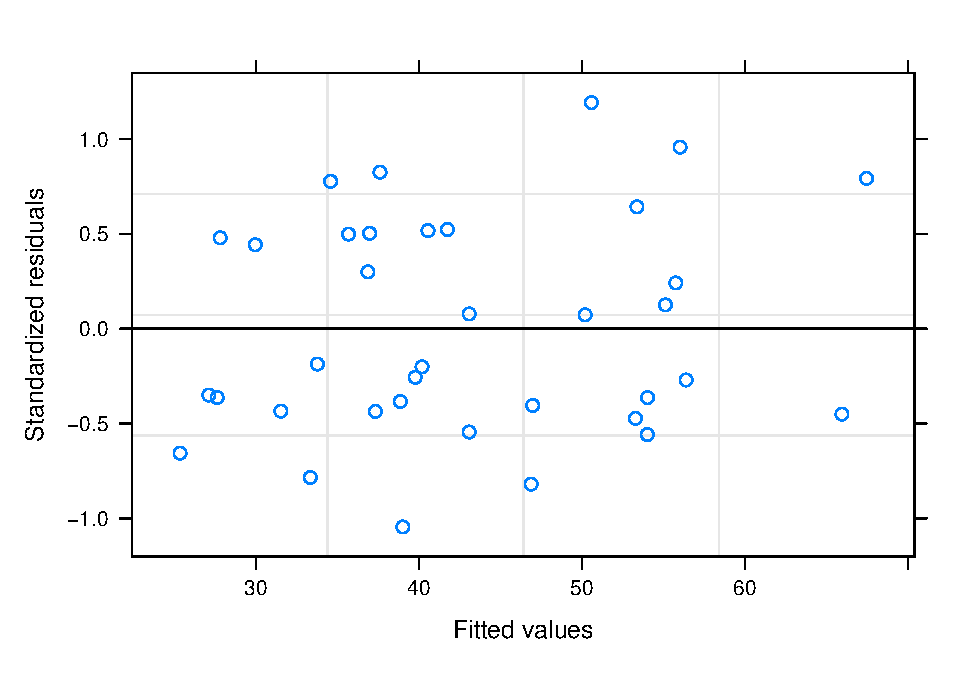
\includegraphics{fig_out/unnamed-chunk-90-1.pdf}

\begin{Shaded}
\begin{Highlighting}[]
\FunctionTok{qqnorm}\NormalTok{(modelo)}
\end{Highlighting}
\end{Shaded}

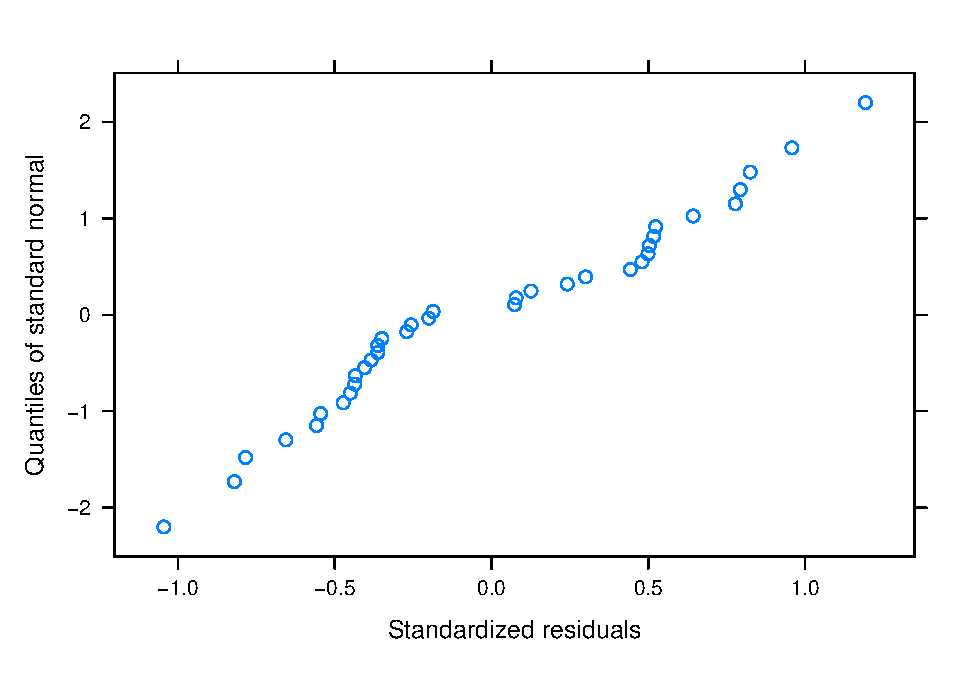
\includegraphics{fig_out/unnamed-chunk-90-2.pdf}

Según estos gráficos, diremos que sí se cumplen las premisas sobre los residuos.

\textbf{Predicciones:}

Para calcular las predicciones nos será útil usar las funciones del paquete \textbf{\texttt{ggeffects}}. Con este paquete se pueden realizar las predicciones de distinto tipo y también graficarlas con el paquete \texttt{ggplot2}.

\begin{Shaded}
\begin{Highlighting}[]
\FunctionTok{library}\NormalTok{(ggeffects)}
\end{Highlighting}
\end{Shaded}

\begin{Shaded}
\begin{Highlighting}[]
\NormalTok{pr.fixed }\OtherTok{\textless{}{-}} \FunctionTok{ggpredict}\NormalTok{(modelo, }\StringTok{"tiempo [all]"}\NormalTok{, }\AttributeTok{type=}\StringTok{"fixed"}\NormalTok{)}
\NormalTok{pr.fixed}
\end{Highlighting}
\end{Shaded}

\begin{verbatim}
# Predicted values of medida

tiempo | Predicted |         95% CI
-----------------------------------
     1 |     32.12 | [29.28, 34.95]
     2 |     49.67 | [44.85, 54.48]
     3 |     47.20 | [41.58, 52.82]

Adjusted for:
* indiv = 0 (population-level)
\end{verbatim}

\begin{Shaded}
\begin{Highlighting}[]
\NormalTok{pr.random }\OtherTok{\textless{}{-}} \FunctionTok{ggpredict}\NormalTok{(modelo, }\StringTok{"tiempo [all]"}\NormalTok{, }\AttributeTok{type=}\StringTok{"random"}\NormalTok{)}
\NormalTok{pr.random}
\end{Highlighting}
\end{Shaded}

\begin{verbatim}
# Predicted values of medida

tiempo
------
     1
     2
     3

Adjusted for:
* indiv = 0 (population-level)
\end{verbatim}

Con el argumento \texttt{type="random"}, el intervalo es más ancho porque no sólo tiene en cuenta el error estándar de las estimaciones de los parámetros sino también la varianza de los efectos aleatorios.

\begin{Shaded}
\begin{Highlighting}[]
\FunctionTok{library}\NormalTok{(gridExtra)}
\FunctionTok{grid.arrange}\NormalTok{(}
    \FunctionTok{plot}\NormalTok{(pr.fixed) }\SpecialCharTok{+} \FunctionTok{ylim}\NormalTok{(}\DecValTok{25}\NormalTok{,}\DecValTok{60}\NormalTok{) }\SpecialCharTok{+} \FunctionTok{ggtitle}\NormalTok{(}\StringTok{"CI: fixed"}\NormalTok{),}
    \FunctionTok{plot}\NormalTok{(pr.random) }\SpecialCharTok{+} \FunctionTok{ylim}\NormalTok{(}\DecValTok{25}\NormalTok{,}\DecValTok{60}\NormalTok{) }\SpecialCharTok{+} \FunctionTok{ggtitle}\NormalTok{(}\StringTok{"CI: random"}\NormalTok{),}
\AttributeTok{nrow=}\DecValTok{1}\NormalTok{, }\AttributeTok{ncol=}\DecValTok{2}\NormalTok{)}
\end{Highlighting}
\end{Shaded}

\textbf{Resultado}

Por lo tanto el modelo final contendrá el tiempo, el tiempo al cuadrado, la contaste y los coeficientes aleatorios. Finalmente, los residuos se puede suponer independientes.

\textbf{Observaciones}

\begin{itemize}
\tightlist
\item
  Se pueden incorporar \textbf{términos splines} en la fórmula usando la función \textbf{\texttt{ns}} del paquete \texttt{spline}. Es útil cuando se tienen muchas medidas repetidas y/o en distintos momentos para los diferentes individuos. Se usa en las fórmulas (argumentos \texttt{fixed} i \texttt{random})
\end{itemize}

\begin{Shaded}
\begin{Highlighting}[]
\FunctionTok{lme}\NormalTok{(respuesta }\SpecialCharTok{\textasciitilde{}} \FunctionTok{ns}\NormalTok{(tiempo), }\AttributeTok{random =} \FunctionTok{ns}\NormalTok{(tiempo) }\SpecialCharTok{|}\NormalTok{ indiv, ...)}
\end{Highlighting}
\end{Shaded}

\textbf{Comparación con las otras técnicas}

A fin de poder comparar los resultados de los modelo LMM con los modelos basados en la suma de cuadrados y en la respuesta multivariante, el tiempo se debe tratar como factor. Fíjate en el uso de \texttt{as.factor} para convertir una variable numérica a factor o variable categórica. Para ello, hay que tener las mismas categorías de tiempo para todos los individuos. Además, tanto los modelos de respuesta multivariable como los basados en suma de cuadrados, asumen la pendiente fija o constante, y la correlación sin estructura.

\begin{center}\rule{0.5\linewidth}{0.5pt}\end{center}

\begin{quote}
\textbf{Nota:} Es importante notar que las técnicas de respuesta multivariable y de suma de cuadrados al tratar la variable tiempo como factor, no se puede distinguir si tiempos de las medidas son o no equiespaiados. Por ejemplo los resultados obtenidos mediante estas dos técnicas serán los mismos tanto si se recogen las medidas a 1h, 2h y 3h, o si se recoge a 1h, 2h y 6h. En cambio, si se desea estudiar el efecto lineal ambas situaciones son muy distintas.
\end{quote}

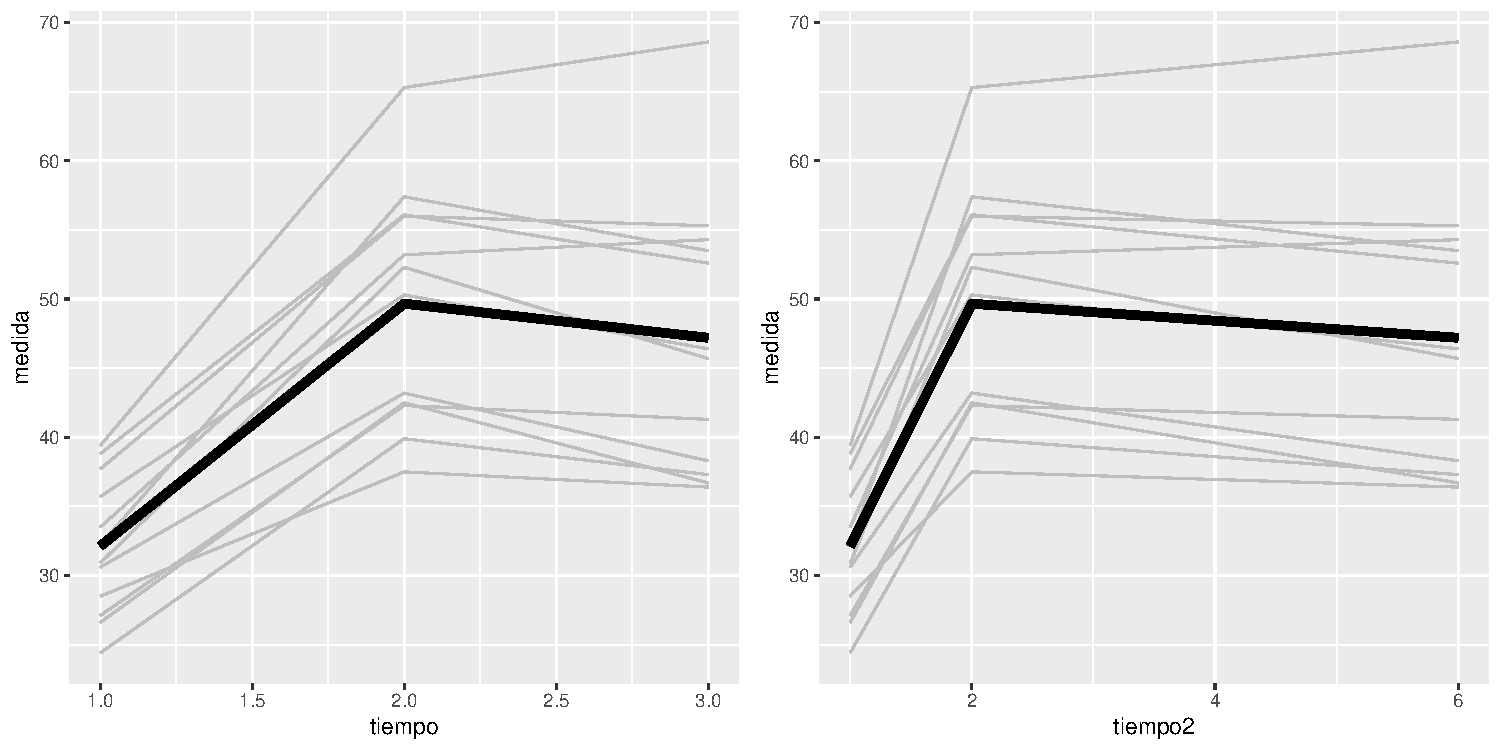
\includegraphics{fig_out/unnamed-chunk-96-1.pdf}

\begin{center}\rule{0.5\linewidth}{0.5pt}\end{center}

\begin{Shaded}
\begin{Highlighting}[]
\NormalTok{modelo }\OtherTok{\textless{}{-}} \FunctionTok{lme}\NormalTok{(}\AttributeTok{fixed =}\NormalTok{ medida }\SpecialCharTok{\textasciitilde{}} \FunctionTok{as.factor}\NormalTok{(tiempo), }
              \AttributeTok{data=}\NormalTok{datos,}
              \AttributeTok{random =} \SpecialCharTok{\textasciitilde{}} \DecValTok{1} \SpecialCharTok{|}\NormalTok{ indiv,}
              \AttributeTok{correlation =} \FunctionTok{corSymm}\NormalTok{()}
\NormalTok{              )}
\FunctionTok{summary}\NormalTok{(modelo)}
\end{Highlighting}
\end{Shaded}

\begin{verbatim}
Linear mixed-effects model fit by REML
  Data: datos 
       AIC      BIC    logLik
  218.5233 230.4954 -101.2616

Random effects:
 Formula: ~1 | indiv
        (Intercept) Residual
StdDev:    7.069756 3.498312

Correlation Structure: General
 Formula: ~1 | indiv 
 Parameter estimate(s):
 Correlation: 
  1      2     
2  0.081       
3 -0.561  0.628
Fixed effects:  medida ~ as.factor(tiempo) 
                      Value Std.Error DF
(Intercept)        32.11667  2.277053 22
as.factor(tiempo)2 17.55000  1.368874 22
as.factor(tiempo)3 15.08333  1.784415 22
                     t-value p-value
(Intercept)        14.104488       0
as.factor(tiempo)2 12.820757       0
as.factor(tiempo)3  8.452817       0
 Correlation: 
                   (Intr) as.()2
as.factor(tiempo)2 -0.301       
as.factor(tiempo)3 -0.392  0.880

Standardized Within-Group Residuals:
        Min          Q1         Med          Q3 
-1.95466422 -0.48588298 -0.07605957  0.47680669 
        Max 
 2.08061488 

Number of Observations: 36
Number of Groups: 12 
\end{verbatim}

\begin{Shaded}
\begin{Highlighting}[]
\FunctionTok{coef}\NormalTok{(}\FunctionTok{summary}\NormalTok{(modelo))}
\end{Highlighting}
\end{Shaded}

\begin{verbatim}
                      Value Std.Error DF
(Intercept)        32.11667  2.277053 22
as.factor(tiempo)2 17.55000  1.368874 22
as.factor(tiempo)3 15.08333  1.784415 22
                     t-value      p-value
(Intercept)        14.104488 1.683824e-12
as.factor(tiempo)2 12.820757 1.104451e-11
as.factor(tiempo)3  8.452817 2.338498e-08
\end{verbatim}

La función \texttt{anova} aplicada a un sólo modelo ajustado es útil para contrastar la significación de un factor de más de una categoría (o posibles interacciones de factores de más de dos categorías).

\begin{Shaded}
\begin{Highlighting}[]
\FunctionTok{anova}\NormalTok{(modelo)}
\end{Highlighting}
\end{Shaded}

\begin{verbatim}
                  numDF denDF  F-value p-value
(Intercept)           1    22 319.4667  <.0001
as.factor(tiempo)     2    22  99.9590  <.0001
\end{verbatim}

\hypertarget{ejemplo-2}{%
\subsection{Ejemplo 2}\label{ejemplo-2}}

Analicemos ahora los datos introducidos en el capítulo anterior en el \protect\hyperlink{Ejercicio2}{ejercicio 2}. Recordemos que en la base de datos ``Ejemplo\_1W1B.csv'' se tienen los datos de un estudio en el que participan 24 individuos randomizados en dos grupos de tratamiento (\texttt{trat}). Como en el anterior ejemplo, para cada invidivuo se miden los niveles a 1, 2 y 3 horas.

\begin{Shaded}
\begin{Highlighting}[]
\NormalTok{datos }\OtherTok{\textless{}{-}} \FunctionTok{read.csv2}\NormalTok{(}\StringTok{"datos/Ejemplo\_1W1B.csv"}\NormalTok{)}
\end{Highlighting}
\end{Shaded}

Como antes, ordenamos por individuo (de 1 a 24) y por tiempo

\begin{Shaded}
\begin{Highlighting}[]
\NormalTok{datos }\OtherTok{\textless{}{-}} \FunctionTok{arrange}\NormalTok{(datos, indiv2, tiempo)}
\end{Highlighting}
\end{Shaded}

\begin{Shaded}
\begin{Highlighting}[]
\NormalTok{modelo }\OtherTok{\textless{}{-}} \FunctionTok{lme}\NormalTok{(}\AttributeTok{fixed =}\NormalTok{ medida }\SpecialCharTok{\textasciitilde{}} \FunctionTok{poly}\NormalTok{(tiempo,}\DecValTok{2}\NormalTok{)}\SpecialCharTok{*}\NormalTok{trat, }
              \AttributeTok{data=}\NormalTok{datos,}
              \AttributeTok{random =} \SpecialCharTok{\textasciitilde{}} \FunctionTok{poly}\NormalTok{(tiempo,}\DecValTok{2}\NormalTok{) }\SpecialCharTok{|}\NormalTok{ indiv2,}
              \AttributeTok{correlation =} \FunctionTok{corAR1}\NormalTok{()}
\NormalTok{              )}
\FunctionTok{summary}\NormalTok{(modelo)}
\end{Highlighting}
\end{Shaded}

\begin{verbatim}
Linear mixed-effects model fit by REML
  Data: datos 
      AIC      BIC   logLik
  386.914 417.5692 -179.457

Random effects:
 Formula: ~poly(tiempo, 2) | indiv2
 Structure: General positive-definite, Log-Cholesky parametrization
                 StdDev    Corr         
(Intercept)       6.528818 (Intr) p(,2)1
poly(tiempo, 2)1 15.016144  0.720       
poly(tiempo, 2)2  5.983554 -0.637 -0.653
Residual          1.290085              

Correlation Structure: AR(1)
 Formula: ~1 | indiv2 
 Parameter estimate(s):
         Phi 
5.458068e-05 
Fixed effects:  medida ~ poly(tiempo, 2) * trat 
                          Value Std.Error DF
(Intercept)            22.16667  4.241672 44
poly(tiempo, 2)1      -35.16063 10.516421 44
poly(tiempo, 2)2       33.10000  5.617817 44
trat                   10.41389  2.682669 22
poly(tiempo, 2)1:trat  43.70542  6.651169 44
poly(tiempo, 2)2:trat -36.56667  3.553020 44
                         t-value p-value
(Intercept)             5.225927  0.0000
poly(tiempo, 2)1       -3.343403  0.0017
poly(tiempo, 2)2        5.891968  0.0000
trat                    3.881914  0.0008
poly(tiempo, 2)1:trat   6.571088  0.0000
poly(tiempo, 2)2:trat -10.291715  0.0000
 Correlation: 
                      (Intr) pl(,2)1 pl(,2)2
poly(tiempo, 2)1       0.659                
poly(tiempo, 2)2      -0.435 -0.414         
trat                  -0.949 -0.625   0.413 
poly(tiempo, 2)1:trat -0.625 -0.949   0.393 
poly(tiempo, 2)2:trat  0.413  0.393  -0.949 
                      trat   p(,2)1:
poly(tiempo, 2)1                    
poly(tiempo, 2)2                    
trat                                
poly(tiempo, 2)1:trat  0.659        
poly(tiempo, 2)2:trat -0.435 -0.414 

Standardized Within-Group Residuals:
        Min          Q1         Med          Q3 
-1.17636054 -0.41451565 -0.05512438  0.37021883 
        Max 
 1.36156358 

Number of Observations: 72
Number of Groups: 24 
\end{verbatim}

\textbf{Nota}:
Si los individuos estuvieran anidados dentro de clusters, se especificaría en el argumento \texttt{random\ =\ \textasciitilde{}\ 1\ \textbar{}\ indiv\ /\ clusters}, donde ``cluster'' sería el nombre de la variable que codifica los clusters.

\textbf{Observación} Para que el modelo quede bien definido no es posible poner la interacción del tiempo y el tratamiento como coeficiente aleatorio. De esta manera se especifican como aleatorios la costante y los coeficientes del tiempo (lineal y cuadrático) para el grupo control.

Como en el anterior ejemplo, contrastamos la significación de los coeficientes aleatorios del tiempo:

\begin{Shaded}
\begin{Highlighting}[]
\FunctionTok{anova}\NormalTok{(modelo, }\FunctionTok{update}\NormalTok{(modelo, }\AttributeTok{random =} \SpecialCharTok{\textasciitilde{}} \DecValTok{1} \SpecialCharTok{|}\NormalTok{ indiv2))}
\end{Highlighting}
\end{Shaded}

\begin{verbatim}
                                     Model df
modelo                                   1 14
update(modelo, random = ~1 | indiv2)     2  9
                                          AIC
modelo                               386.9140
update(modelo, random = ~1 | indiv2) 393.6099
                                          BIC
modelo                               417.5692
update(modelo, random = ~1 | indiv2) 413.3168
                                       logLik
modelo                               -179.457
update(modelo, random = ~1 | indiv2) -187.805
                                       Test
modelo                                     
update(modelo, random = ~1 | indiv2) 1 vs 2
                                      L.Ratio
modelo                                       
update(modelo, random = ~1 | indiv2) 16.69594
                                     p-value
modelo                                      
update(modelo, random = ~1 | indiv2)  0.0051
\end{verbatim}

Según el criterio AIC o BIC, el modelo con pendientes aleatorias es mejor.

Luego, contrastamos si se puede simplificar la matriz de correlaciones de los efectos aleatorios:

\begin{Shaded}
\begin{Highlighting}[]
\FunctionTok{anova}\NormalTok{(modelo, }\FunctionTok{update}\NormalTok{(modelo, }\AttributeTok{random =} \FunctionTok{list}\NormalTok{(}\AttributeTok{indiv2=}\FunctionTok{pdDiag}\NormalTok{(}\SpecialCharTok{\textasciitilde{}}\FunctionTok{poly}\NormalTok{(tiempo,}\DecValTok{2}\NormalTok{)))))}
\end{Highlighting}
\end{Shaded}

\begin{verbatim}
                                                                 Model
modelo                                                               1
update(modelo, random = list(indiv2 = pdDiag(~poly(tiempo, 2))))     2
                                                                 df
modelo                                                           14
update(modelo, random = list(indiv2 = pdDiag(~poly(tiempo, 2)))) 11
                                                                      AIC
modelo                                                           386.9140
update(modelo, random = list(indiv2 = pdDiag(~poly(tiempo, 2)))) 397.1845
                                                                      BIC
modelo                                                           417.5692
update(modelo, random = list(indiv2 = pdDiag(~poly(tiempo, 2)))) 421.2707
                                                                    logLik
modelo                                                           -179.4570
update(modelo, random = list(indiv2 = pdDiag(~poly(tiempo, 2)))) -187.5922
                                                                   Test
modelo                                                                 
update(modelo, random = list(indiv2 = pdDiag(~poly(tiempo, 2)))) 1 vs 2
                                                                  L.Ratio
modelo                                                                   
update(modelo, random = list(indiv2 = pdDiag(~poly(tiempo, 2)))) 16.27047
                                                                 p-value
modelo                                                                  
update(modelo, random = list(indiv2 = pdDiag(~poly(tiempo, 2))))   0.001
\end{verbatim}

El test LRT es significativo (p-valor \textless{} 0.05). Por lo tanto nos quedamos con el modelo más complejo que supone que hay correlación entre los efectos aleatorios.

Seguidamente, miramos si se puede simplificar la matriz de correlaciones de los errores.

\begin{Shaded}
\begin{Highlighting}[]
\FunctionTok{anova}\NormalTok{(modelo, }\FunctionTok{update}\NormalTok{(modelo, }\AttributeTok{correlation=}\ConstantTok{NULL}\NormalTok{))}
\end{Highlighting}
\end{Shaded}

\begin{verbatim}
                                   Model df
modelo                                 1 14
update(modelo, correlation = NULL)     2 13
                                       AIC
modelo                             386.914
update(modelo, correlation = NULL) 384.914
                                        BIC
modelo                             417.5692
update(modelo, correlation = NULL) 413.3795
                                     logLik
modelo                             -179.457
update(modelo, correlation = NULL) -179.457
                                     Test
modelo                                   
update(modelo, correlation = NULL) 1 vs 2
                                        L.Ratio
modelo                                         
update(modelo, correlation = NULL) 1.063989e-08
                                   p-value
modelo                                    
update(modelo, correlation = NULL)  0.9999
\end{verbatim}

Sí que se puede suponer que hay indipendencia entre los residuos.

\begin{Shaded}
\begin{Highlighting}[]
\NormalTok{modelo }\OtherTok{\textless{}{-}} \FunctionTok{update}\NormalTok{(modelo, }\AttributeTok{correlation=}\ConstantTok{NULL}\NormalTok{)}
\end{Highlighting}
\end{Shaded}

Por lo tanto el modelo final, que supone independencia entre residuos, tiene la siguiente estimación de los efectos fijos:

\begin{Shaded}
\begin{Highlighting}[]
\FunctionTok{coef}\NormalTok{(}\FunctionTok{summary}\NormalTok{(modelo))}
\end{Highlighting}
\end{Shaded}

\begin{verbatim}
                          Value Std.Error DF
(Intercept)            22.16667  4.241667 44
poly(tiempo, 2)1      -35.16063 10.516526 44
poly(tiempo, 2)2       33.10000  5.617838 44
trat                   10.41389  2.682666 22
poly(tiempo, 2)1:trat  43.70542  6.651235 44
poly(tiempo, 2)2:trat -36.56667  3.553033 44
                         t-value      p-value
(Intercept)             5.225932 4.556683e-06
poly(tiempo, 2)1       -3.343370 1.698154e-03
poly(tiempo, 2)2        5.891946 4.863408e-07
trat                    3.881918 8.040480e-04
poly(tiempo, 2)1:trat   6.571023 4.876727e-08
poly(tiempo, 2)2:trat -10.291677 2.732020e-13
\end{verbatim}

Vemos como el efecto del tiempo para el grupo control no llega a ser significativo (p-valores \textgreater0.05) tanto para su componente lineal como cuadrático. Hay efecto del tratamiento en el momento basal (\texttt{trat2}).

Si queremos ver el efecto del tiempo para el grupo 2, hay que cambiar su categoría de referencia.

\begin{Shaded}
\begin{Highlighting}[]
\NormalTok{datos}\SpecialCharTok{$}\NormalTok{trat }\OtherTok{\textless{}{-}} \FunctionTok{relevel}\NormalTok{(}\FunctionTok{factor}\NormalTok{(datos}\SpecialCharTok{$}\NormalTok{trat),}\DecValTok{2}\NormalTok{)}
\FunctionTok{coef}\NormalTok{(}\FunctionTok{summary}\NormalTok{(}\FunctionTok{update}\NormalTok{(modelo)))}
\end{Highlighting}
\end{Shaded}

\begin{verbatim}
                           Value Std.Error DF
(Intercept)             42.99444  1.896932 44
poly(tiempo, 2)1        52.25020  4.703133 44
poly(tiempo, 2)2       -40.03333  2.512374 44
trat1                  -10.41389  2.682666 22
poly(tiempo, 2)1:trat1 -43.70542  6.651235 44
poly(tiempo, 2)2:trat1  36.56667  3.553033 44
                          t-value      p-value
(Intercept)             22.665259 6.756030e-26
poly(tiempo, 2)1        11.109658 2.358252e-14
poly(tiempo, 2)2       -15.934465 6.870764e-20
trat1                   -3.881917 8.040486e-04
poly(tiempo, 2)1:trat1  -6.571023 4.876723e-08
poly(tiempo, 2)2:trat1  10.291676 2.732023e-13
\end{verbatim}

Vemos que para el grupo 2 tanto la componente lineal como la cuadrática del tiempo son significativas.

Con la siguiente matriz de varianzas y covarianzas de los efectos aleatorios:

\begin{Shaded}
\begin{Highlighting}[]
\FunctionTok{getVarCov}\NormalTok{(modelo)}
\end{Highlighting}
\end{Shaded}

\begin{verbatim}
Random effects variance covariance matrix
                 (Intercept) poly(tiempo, 2)1
(Intercept)           42.625           70.566
poly(tiempo, 2)1      70.566          225.490
poly(tiempo, 2)2     -24.889          -58.669
                 poly(tiempo, 2)2
(Intercept)               -24.889
poly(tiempo, 2)1          -58.669
poly(tiempo, 2)2           35.802
  Standard Deviations: 6.5288 15.016 5.9835 
\end{verbatim}

Y varianza de los residuos

\begin{Shaded}
\begin{Highlighting}[]
\FunctionTok{sigma}\NormalTok{(modelo)}\SpecialCharTok{\^{}}\DecValTok{2}
\end{Highlighting}
\end{Shaded}

\begin{verbatim}
[1] 1.664273
\end{verbatim}

Por último, validamos el modelo

\begin{Shaded}
\begin{Highlighting}[]
\FunctionTok{par}\NormalTok{(}\AttributeTok{mfrow=}\FunctionTok{c}\NormalTok{(}\DecValTok{1}\NormalTok{,}\DecValTok{2}\NormalTok{))}
\FunctionTok{plot}\NormalTok{(modelo)}
\end{Highlighting}
\end{Shaded}

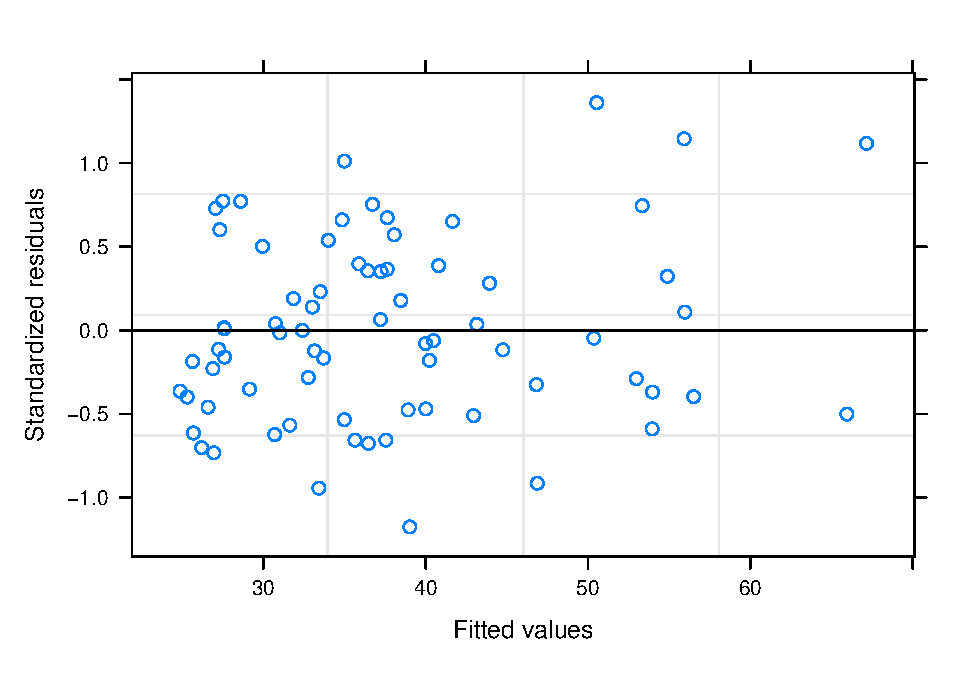
\includegraphics{fig_out/unnamed-chunk-110-1.pdf}

\begin{Shaded}
\begin{Highlighting}[]
\FunctionTok{qqnorm}\NormalTok{(modelo)}
\end{Highlighting}
\end{Shaded}

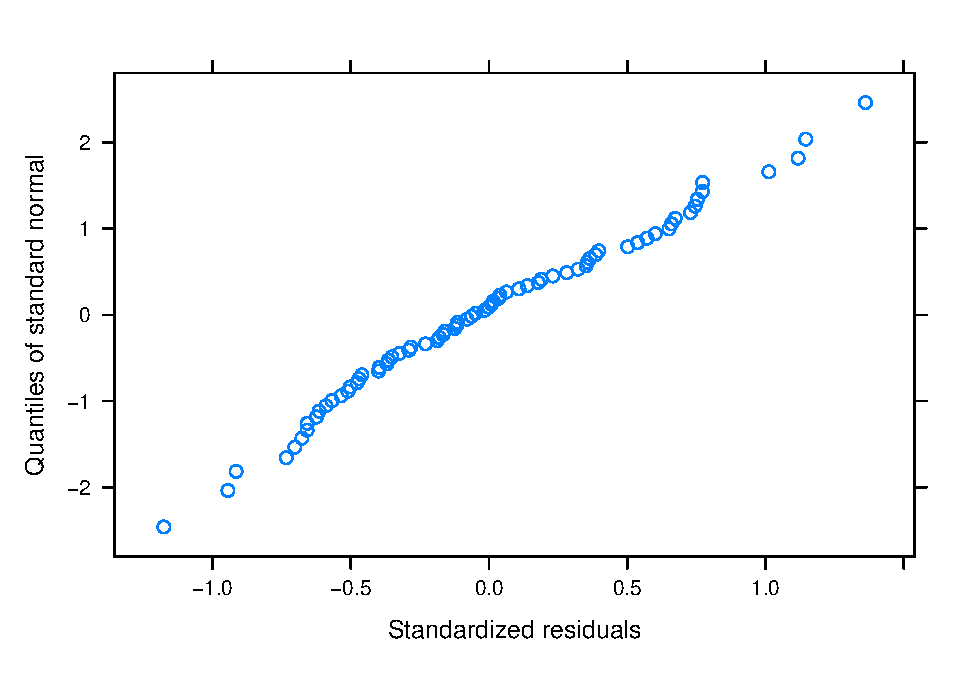
\includegraphics{fig_out/unnamed-chunk-110-2.pdf}

Según los gráficos, parece que sí que se cumplen las premisas sobre los residuos.

\textbf{Predicciones}

\begin{Shaded}
\begin{Highlighting}[]
\NormalTok{pr }\OtherTok{\textless{}{-}} \FunctionTok{ggpredict}\NormalTok{(modelo, }\AttributeTok{terms =} \FunctionTok{c}\NormalTok{(}\StringTok{"tiempo [all]"}\NormalTok{, }\StringTok{"trat"}\NormalTok{))}
\NormalTok{pr}
\end{Highlighting}
\end{Shaded}

\begin{verbatim}
# Predicted values of medida

# trat = 1

tiempo | Predicted |         95% CI
-----------------------------------
     1 |     31.06 | [28.17, 33.95]
     2 |     33.16 | [29.02, 37.30]
     3 |     33.52 | [29.00, 38.05]

# trat = 2

tiempo | Predicted |         95% CI
-----------------------------------
     1 |     32.12 | [29.22, 35.01]
     2 |     49.67 | [45.53, 53.81]
     3 |     47.20 | [42.67, 51.73]

Adjusted for:
* indiv2 = 0 (population-level)
\end{verbatim}

\begin{Shaded}
\begin{Highlighting}[]
\FunctionTok{plot}\NormalTok{(pr, }\AttributeTok{add.data =} \ConstantTok{TRUE}\NormalTok{)}
\end{Highlighting}
\end{Shaded}

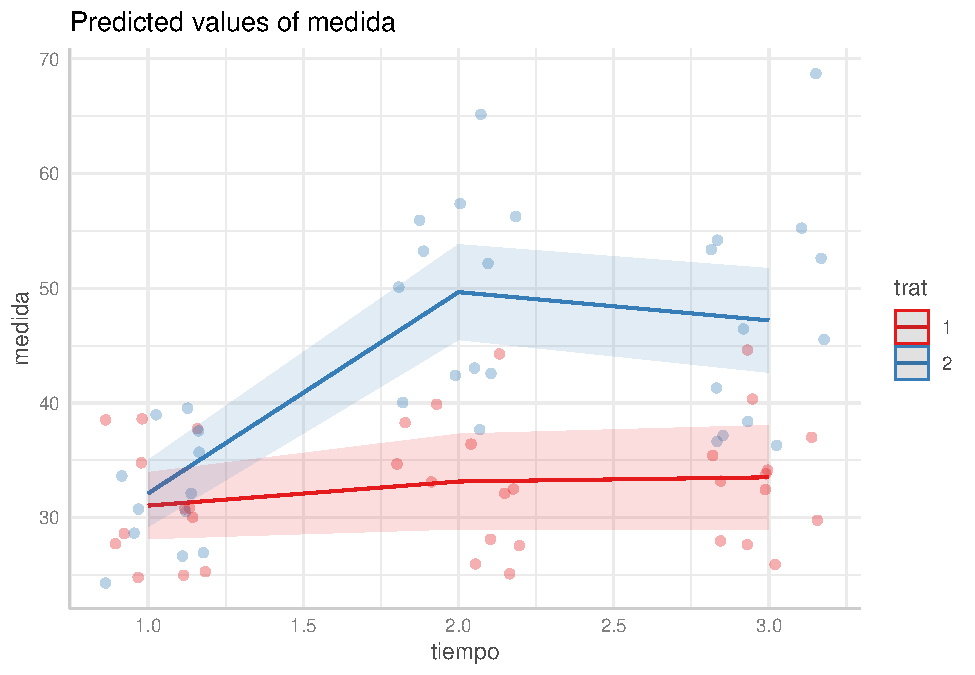
\includegraphics{fig_out/unnamed-chunk-111-1.pdf}

\hypertarget{ejemplo-3}{%
\subsection{Ejemplo 3}\label{ejemplo-3}}

Finalmente, analicemos ahora los datos introducidos en el capítulo anterior en el \protect\hyperlink{Ejercicio3}{ejercicio 3}. En un estudio se quieren comparar el efecto de régimen de ejercicio sobre el sobrepeso. Para ello se reclutan 100 personas. A la mitad se le asigna el régimen y al resto se le hacen algunas recomendaciones (grupo control). Se mide el índice de masa corporal justo antes de empezar el estudio (momento basal), y al cabo de 1, 2 y 3 semanas. Como la edad es una variable importante para predecir el IMC también se registra.

Los datos los encontrarás en el fichero ``imc.csv''

En este ejemplo, vemos como en algunos de los individuos nos falta alguna medida en a partir de la primera semana. Por este motivo usaremos la técnica de los LMM.

\begin{Shaded}
\begin{Highlighting}[]
\NormalTok{datos }\OtherTok{\textless{}{-}} \FunctionTok{read.csv2}\NormalTok{(}\StringTok{"datos/imc.csv"}\NormalTok{)}
\end{Highlighting}
\end{Shaded}

Nos aseguramos que los datos estén ordenados por individuo y tiempo

\begin{Shaded}
\begin{Highlighting}[]
\NormalTok{datos }\OtherTok{\textless{}{-}} \FunctionTok{arrange}\NormalTok{(datos, indiv, tiempo)}
\end{Highlighting}
\end{Shaded}

Recodificamos nuestra variable tratamiento:

\begin{Shaded}
\begin{Highlighting}[]
\NormalTok{datos}\SpecialCharTok{$}\NormalTok{tx }\OtherTok{\textless{}{-}} \FunctionTok{factor}\NormalTok{(datos}\SpecialCharTok{$}\NormalTok{tx, }\DecValTok{1}\SpecialCharTok{:}\DecValTok{2}\NormalTok{, }\FunctionTok{c}\NormalTok{(}\StringTok{"Control"}\NormalTok{, }\StringTok{"Tratados"}\NormalTok{))}
\FunctionTok{summary}\NormalTok{(datos)}
\end{Highlighting}
\end{Shaded}

\begin{verbatim}
   respuesta         indiv            tiempo    
 Min.   : 9.80   Min.   :  1.00   Min.   :0.00  
 1st Qu.:27.02   1st Qu.: 25.75   1st Qu.:0.75  
 Median :30.75   Median : 50.50   Median :1.50  
 Mean   :30.46   Mean   : 50.50   Mean   :1.50  
 3rd Qu.:34.60   3rd Qu.: 75.25   3rd Qu.:2.25  
 Max.   :43.70   Max.   :100.00   Max.   :3.00  
 NA's   :50                                     
      edad              tx     
 Min.   :25.00   Control :200  
 1st Qu.:43.00   Tratados:200  
 Median :49.00                 
 Mean   :49.03                 
 3rd Qu.:57.00                 
 Max.   :69.00                 
                               
\end{verbatim}

Recordemos también que estos datos no puedieron ser analizados con métodos tradicionales ya que tienen inviduos con datos faltantes

\begin{Shaded}
\begin{Highlighting}[]
\FunctionTok{sum}\NormalTok{(}\FunctionTok{with}\NormalTok{(datos, }\FunctionTok{tapply}\NormalTok{(}\FunctionTok{is.na}\NormalTok{(respuesta), indiv, any)))}
\end{Highlighting}
\end{Shaded}

\begin{verbatim}
[1] 42
\end{verbatim}

Elimino las observaciones con valores missing (que no los individuos!)

\begin{Shaded}
\begin{Highlighting}[]
\NormalTok{datos }\OtherTok{\textless{}{-}} \FunctionTok{subset}\NormalTok{(datos, }\SpecialCharTok{!}\FunctionTok{is.na}\NormalTok{(respuesta))}
\CommentTok{\# número de individuos con 2, 3 o 4 medidas válidas.}
\FunctionTok{table}\NormalTok{(}\FunctionTok{table}\NormalTok{(datos}\SpecialCharTok{$}\NormalTok{indiv))}
\end{Highlighting}
\end{Shaded}

\begin{verbatim}
 2  3  4 
 8 34 58 
\end{verbatim}

Como siempre, hagamos una visualización de los datos

\begin{Shaded}
\begin{Highlighting}[]
\FunctionTok{library}\NormalTok{(ggplot2)}
\NormalTok{p }\OtherTok{\textless{}{-}} \FunctionTok{ggplot}\NormalTok{(}\AttributeTok{data =}\NormalTok{ datos, }\FunctionTok{aes}\NormalTok{(}\AttributeTok{x =}\NormalTok{ tiempo, }\AttributeTok{y =}\NormalTok{ respuesta, }\AttributeTok{group =}\NormalTok{ indiv))}
\NormalTok{p }\OtherTok{\textless{}{-}}\NormalTok{ p }\SpecialCharTok{+} \FunctionTok{geom\_line}\NormalTok{(}\AttributeTok{col=}\StringTok{"grey"}\NormalTok{) }\SpecialCharTok{+} \FunctionTok{stat\_summary}\NormalTok{(}\FunctionTok{aes}\NormalTok{(}\AttributeTok{group =} \DecValTok{1}\NormalTok{),}
    \AttributeTok{geom =} \StringTok{"line"}\NormalTok{, }\AttributeTok{fun =}\NormalTok{ mean, }\AttributeTok{size=}\DecValTok{2}\NormalTok{)}
\NormalTok{p }\SpecialCharTok{+} \FunctionTok{facet\_grid}\NormalTok{( }\SpecialCharTok{\textasciitilde{}}\NormalTok{ tx)}
\end{Highlighting}
\end{Shaded}

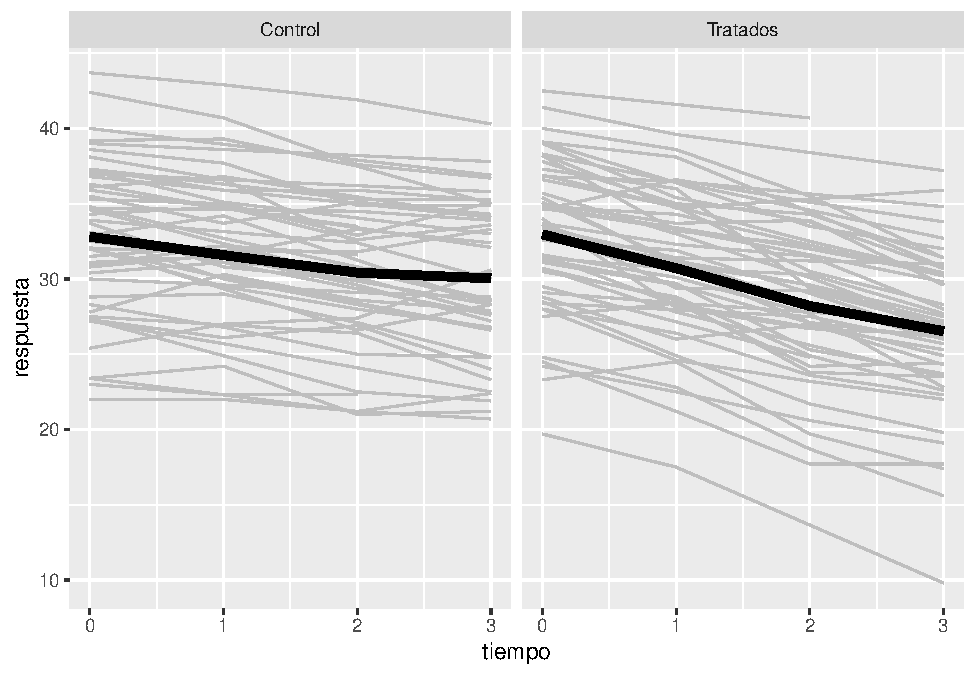
\includegraphics{fig_out/unnamed-chunk-117-1.pdf}

\hypertarget{anuxe1lisis-del-grupo-control}{%
\subsubsection{Análisis del grupo control}\label{anuxe1lisis-del-grupo-control}}

Si analizamos sólo el grupo control, se trata de un diseño 1W con una covariable (edad).

\begin{Shaded}
\begin{Highlighting}[]
\NormalTok{datos }\OtherTok{\textless{}{-}} \FunctionTok{subset}\NormalTok{(datos, tx}\SpecialCharTok{==}\StringTok{\textquotesingle{}Control\textquotesingle{}}\NormalTok{)}
\NormalTok{datos }\OtherTok{\textless{}{-}} \FunctionTok{na.omit}\NormalTok{(datos)}
\end{Highlighting}
\end{Shaded}

Ajustamos el modelo más completo, con la edad y el tiempo hasta el término cúbico ya que tenemos cuatro medidas.

\begin{Shaded}
\begin{Highlighting}[]
\FunctionTok{library}\NormalTok{(nlme)}
\NormalTok{modelo }\OtherTok{\textless{}{-}} \FunctionTok{lme}\NormalTok{(respuesta }\SpecialCharTok{\textasciitilde{}} \FunctionTok{poly}\NormalTok{(tiempo,}\DecValTok{3}\NormalTok{) }\SpecialCharTok{+}\NormalTok{ edad, }
              \AttributeTok{random=} \SpecialCharTok{\textasciitilde{}} \FunctionTok{poly}\NormalTok{(tiempo,}\DecValTok{3}\NormalTok{) }\SpecialCharTok{|}\NormalTok{ indiv, }
              \AttributeTok{data=}\NormalTok{datos, }
              \CommentTok{\#correlation = corSymm(), \# sin estructura}
              \AttributeTok{correlation=}\FunctionTok{corCAR1}\NormalTok{(}\AttributeTok{form =} \SpecialCharTok{\textasciitilde{}}\NormalTok{ tiempo }\SpecialCharTok{|}\NormalTok{ indiv),}
              \AttributeTok{control=}\FunctionTok{lmeControl}\NormalTok{(}\AttributeTok{opt=}\StringTok{"optim"}\NormalTok{))}
\FunctionTok{summary}\NormalTok{(modelo)}
\end{Highlighting}
\end{Shaded}

\begin{verbatim}
Linear mixed-effects model fit by REML
  Data: datos 
       AIC      BIC    logLik
  672.3888 724.9826 -319.1944

Random effects:
 Formula: ~poly(tiempo, 3) | indiv
 Structure: General positive-definite, Log-Cholesky parametrization
                 StdDev     Corr                
(Intercept)       2.1235727 (Intr) p(,3)1 p(,3)2
poly(tiempo, 3)1 10.8729435 -0.143              
poly(tiempo, 3)2  5.3455110  0.317  0.071       
poly(tiempo, 3)3  4.2631158  0.057 -0.026  0.193
Residual          0.5431964                     

Correlation Structure: Continuous AR(1)
 Formula: ~tiempo | indiv 
 Parameter estimate(s):
      Phi 
0.1999231 
Fixed effects:  respuesta ~ poly(tiempo, 3) + edad 
                      Value Std.Error  DF
(Intercept)       10.409728 1.4770932 115
poly(tiempo, 3)1 -15.045596 1.6657189 115
poly(tiempo, 3)2  -0.518758 1.0075975 115
poly(tiempo, 3)3   1.865008 0.8918255 115
edad               0.432945 0.0297828  48
                   t-value p-value
(Intercept)       7.047442  0.0000
poly(tiempo, 3)1 -9.032494  0.0000
poly(tiempo, 3)2 -0.514846  0.6076
poly(tiempo, 3)3  2.091225  0.0387
edad             14.536718  0.0000
 Correlation: 
                 (Intr) p(,3)1 p(,3)2 p(,3)3
poly(tiempo, 3)1 -0.024                     
poly(tiempo, 3)2  0.081  0.089              
poly(tiempo, 3)3  0.012 -0.041  0.149       
edad             -0.978 -0.001 -0.037 -0.003

Standardized Within-Group Residuals:
         Min           Q1          Med 
-1.025920132 -0.293663743 -0.008367651 
          Q3          Max 
 0.290693758  1.093099300 

Number of Observations: 168
Number of Groups: 50 
\end{verbatim}

El modelo de correlación sin estructura no converge (NOTA: intentad ejecutar el mismo código cambiando la correlación que tiene por la que está comentada). Es normal ya que tenemos distintas medidas.

Es importante especificar la AR(1) continua \texttt{corCAR1} ya que tenemos algunos individuos con datos faltantes en algunas de sus medidas. Luego el tiempo que ha pasado entre las medidas disponibles hay que tenerlo en cuenta.

Fíjate en la varianza de los efectos aleatorios, sobretodo en la constante si en el modelo no ponemos la edad,

\begin{Shaded}
\begin{Highlighting}[]
\NormalTok{modelo0 }\OtherTok{\textless{}{-}} \FunctionTok{update}\NormalTok{(modelo, }\AttributeTok{fixed =}\NormalTok{ . }\SpecialCharTok{\textasciitilde{}}\NormalTok{ . }\SpecialCharTok{{-}}\NormalTok{edad)}
\FunctionTok{getVarCov}\NormalTok{(modelo)}
\end{Highlighting}
\end{Shaded}

\begin{verbatim}
Random effects variance covariance matrix
                 (Intercept) poly(tiempo, 3)1
(Intercept)           4.5096          -3.2917
poly(tiempo, 3)1     -3.2917         118.2200
poly(tiempo, 3)2      3.6035           4.1274
poly(tiempo, 3)3      0.5144          -1.1839
                 poly(tiempo, 3)2
(Intercept)                3.6035
poly(tiempo, 3)1           4.1274
poly(tiempo, 3)2          28.5740
poly(tiempo, 3)3           4.4056
                 poly(tiempo, 3)3
(Intercept)                0.5144
poly(tiempo, 3)1          -1.1839
poly(tiempo, 3)2           4.4056
poly(tiempo, 3)3          18.1740
  Standard Deviations: 2.1236 10.873 5.3455 4.2631 
\end{verbatim}

\begin{Shaded}
\begin{Highlighting}[]
\FunctionTok{getVarCov}\NormalTok{(modelo0) }\CommentTok{\# sin la edad}
\end{Highlighting}
\end{Shaded}

\begin{verbatim}
Random effects variance covariance matrix
                 (Intercept) poly(tiempo, 3)1
(Intercept)         22.65700         -2.56910
poly(tiempo, 3)1    -2.56910        108.79000
poly(tiempo, 3)2     0.79669          2.88170
poly(tiempo, 3)3     0.60630          0.23627
                 poly(tiempo, 3)2
(Intercept)               0.79669
poly(tiempo, 3)1          2.88170
poly(tiempo, 3)2         20.71700
poly(tiempo, 3)3          3.90920
                 poly(tiempo, 3)3
(Intercept)               0.60630
poly(tiempo, 3)1          0.23627
poly(tiempo, 3)2          3.90920
poly(tiempo, 3)3         13.19500
  Standard Deviations: 4.76 10.43 4.5516 3.6326 
\end{verbatim}

Es importante poner la edad ya que si no, la varianza de los efectos aleatorios quedan infladas y la inferencia no es válida.

\textbf{Contraste de los efectos aleatorios}

\begin{Shaded}
\begin{Highlighting}[]
\FunctionTok{anova}\NormalTok{(modelo, }\FunctionTok{update}\NormalTok{(modelo, }\AttributeTok{random=} \SpecialCharTok{\textasciitilde{}} \DecValTok{1} \SpecialCharTok{|}\NormalTok{ indiv))}
\end{Highlighting}
\end{Shaded}

\begin{verbatim}
                                    Model df
modelo                                  1 17
update(modelo, random = ~1 | indiv)     2  8
                                         AIC
modelo                              672.3888
update(modelo, random = ~1 | indiv) 662.1079
                                         BIC
modelo                              724.9826
update(modelo, random = ~1 | indiv) 686.8579
                                       logLik
modelo                              -319.1944
update(modelo, random = ~1 | indiv) -323.0539
                                      Test
modelo                                    
update(modelo, random = ~1 | indiv) 1 vs 2
                                     L.Ratio
modelo                                      
update(modelo, random = ~1 | indiv) 7.719062
                                    p-value
modelo                                     
update(modelo, random = ~1 | indiv)  0.5627
\end{verbatim}

Nos quedamos con el modelo con los coeficientes del tiempo fijos:

\begin{Shaded}
\begin{Highlighting}[]
\NormalTok{modelo }\OtherTok{\textless{}{-}} \FunctionTok{update}\NormalTok{(modelo, }\AttributeTok{random=} \SpecialCharTok{\textasciitilde{}} \DecValTok{1} \SpecialCharTok{|}\NormalTok{ indiv)}
\end{Highlighting}
\end{Shaded}

\begin{quote}
\textbf{Observación} Fíjate en el valor de \(\phi\) de la matriz de correlaciones de los errores: al considerar el coeficiente del tiempo como fijo, ha pasado de ser cero a un valor alto. Al considerar el coeficiente aleatorio en cierta manera se inducía una estructura de AR entre las observaciones y ya no hacía falta considerar los errores correlacionados. Por esto, el orden en que se simplifica el modelo es importante.
\end{quote}

Si queremos \textbf{contrastar si la constante es aletoria} se compara el modelo con todos los efectos fijos. Así que ya no se podrá usar la función \texttt{lme} sino que se usará la función \texttt{gls} en su lugar.

\begin{Shaded}
\begin{Highlighting}[]
\NormalTok{modelo.gls }\OtherTok{\textless{}{-}} \FunctionTok{gls}\NormalTok{(respuesta }\SpecialCharTok{\textasciitilde{}} \FunctionTok{poly}\NormalTok{(tiempo,}\DecValTok{3}\NormalTok{) }\SpecialCharTok{+}\NormalTok{ edad, }
                  \AttributeTok{data=}\NormalTok{datos, }
                  \AttributeTok{correlation=}\FunctionTok{corCAR1}\NormalTok{(}\AttributeTok{form =} \SpecialCharTok{\textasciitilde{}}\NormalTok{ tiempo }\SpecialCharTok{|}\NormalTok{indiv))}
\FunctionTok{summary}\NormalTok{(modelo.gls)}
\end{Highlighting}
\end{Shaded}

\begin{verbatim}
Generalized least squares fit by REML
  Model: respuesta ~ poly(tiempo, 3) + edad 
  Data: datos 
       AIC      BIC    logLik
  660.2088 681.8651 -323.1044

Correlation Structure: Continuous AR(1)
 Formula: ~tiempo | indiv 
 Parameter estimate(s):
      Phi 
0.8409838 

Coefficients:
                      Value Std.Error   t-value
(Intercept)       10.743564 1.5857081  6.775247
poly(tiempo, 3)1 -15.049949 1.6527760 -9.105861
poly(tiempo, 3)2  -0.382757 1.0563295 -0.362347
poly(tiempo, 3)3   1.978662 0.8789044  2.251283
edad               0.425951 0.0319656 13.325311
                 p-value
(Intercept)       0.0000
poly(tiempo, 3)1  0.0000
poly(tiempo, 3)2  0.7176
poly(tiempo, 3)3  0.0257
edad              0.0000

 Correlation: 
                 (Intr) p(,3)1 p(,3)2 p(,3)3
poly(tiempo, 3)1  0.001                     
poly(tiempo, 3)2 -0.022  0.019              
poly(tiempo, 3)3  0.003 -0.121  0.024       
edad             -0.980 -0.002 -0.008 -0.001

Standardized residuals:
        Min          Q1         Med          Q3 
-2.39865570 -0.70572628 -0.01464924  0.74989249 
        Max 
 2.07647314 

Residual standard error: 2.492824 
Degrees of freedom: 168 total; 163 residual
\end{verbatim}

\begin{Shaded}
\begin{Highlighting}[]
\FunctionTok{summary}\NormalTok{(modelo)}
\end{Highlighting}
\end{Shaded}

\begin{verbatim}
Linear mixed-effects model fit by REML
  Data: datos 
       AIC      BIC    logLik
  662.1079 686.8579 -323.0539

Random effects:
 Formula: ~1 | indiv
        (Intercept) Residual
StdDev:   0.8028047 2.378488

Correlation Structure: Continuous AR(1)
 Formula: ~tiempo | indiv 
 Parameter estimate(s):
      Phi 
0.8266025 
Fixed effects:  respuesta ~ poly(tiempo, 3) + edad 
                      Value Std.Error  DF
(Intercept)       10.738507 1.6033545 115
poly(tiempo, 3)1 -15.048689 1.6348726 115
poly(tiempo, 3)2  -0.382488 1.0548435 115
poly(tiempo, 3)3   1.978466 0.8786767 115
edad               0.426057 0.0323229  48
                   t-value p-value
(Intercept)       6.697525  0.0000
poly(tiempo, 3)1 -9.204808  0.0000
poly(tiempo, 3)2 -0.362602  0.7176
poly(tiempo, 3)3  2.251643  0.0262
edad             13.181289  0.0000
 Correlation: 
                 (Intr) p(,3)1 p(,3)2 p(,3)3
poly(tiempo, 3)1  0.001                     
poly(tiempo, 3)2 -0.020  0.019              
poly(tiempo, 3)3  0.003 -0.122  0.024       
edad             -0.980 -0.002 -0.008 -0.001

Standardized Within-Group Residuals:
        Min          Q1         Med          Q3 
-2.25670886 -0.66026076  0.01991706  0.66013218 
        Max 
 1.92440305 

Number of Observations: 168
Number of Groups: 50 
\end{verbatim}

\begin{Shaded}
\begin{Highlighting}[]
\FunctionTok{anova}\NormalTok{(modelo, modelo.gls)}
\end{Highlighting}
\end{Shaded}

\begin{verbatim}
           Model df      AIC      BIC    logLik
modelo         1  8 662.1079 686.8579 -323.0539
modelo.gls     2  7 660.2088 681.8651 -323.1044
             Test   L.Ratio p-value
modelo                             
modelo.gls 1 vs 2 0.1009386  0.7507
\end{verbatim}

Los dos modelos no están anidados. Así que a parte del p-valor del LRT también miraremos el AIC y el BIC. Bajo los tres criterios nos decantamos por el modelo con la constante aleatoria.

\textbf{Estructura de correlación de los errores}

Comparamos con la matriz de independencia

\begin{Shaded}
\begin{Highlighting}[]
\FunctionTok{anova}\NormalTok{(modelo, }\FunctionTok{update}\NormalTok{(modelo, }\AttributeTok{correlation=}\ConstantTok{NULL}\NormalTok{))}
\end{Highlighting}
\end{Shaded}

\begin{verbatim}
                                   Model df
modelo                                 1  8
update(modelo, correlation = NULL)     2  7
                                        AIC
modelo                             662.1079
update(modelo, correlation = NULL) 677.6130
                                        BIC
modelo                             686.8579
update(modelo, correlation = NULL) 699.2693
                                      logLik
modelo                             -323.0539
update(modelo, correlation = NULL) -331.8065
                                     Test
modelo                                   
update(modelo, correlation = NULL) 1 vs 2
                                    L.Ratio
modelo                                     
update(modelo, correlation = NULL) 17.50515
                                   p-value
modelo                                    
update(modelo, correlation = NULL)  <.0001
\end{verbatim}

Nos quedamos con la estructura AR1

\textbf{Contraste de los efectos fijos}

\begin{Shaded}
\begin{Highlighting}[]
\FunctionTok{coef}\NormalTok{(}\FunctionTok{summary}\NormalTok{(modelo))}
\end{Highlighting}
\end{Shaded}

\begin{verbatim}
                       Value Std.Error  DF
(Intercept)       10.7385066 1.6033545 115
poly(tiempo, 3)1 -15.0486889 1.6348726 115
poly(tiempo, 3)2  -0.3824884 1.0548435 115
poly(tiempo, 3)3   1.9784662 0.8786767 115
edad               0.4260575 0.0323229  48
                   t-value      p-value
(Intercept)       6.697525 8.187045e-10
poly(tiempo, 3)1 -9.204808 1.848306e-15
poly(tiempo, 3)2 -0.362602 7.175678e-01
poly(tiempo, 3)3  2.251643 2.624396e-02
edad             13.181289 1.441756e-17
\end{verbatim}

Vemos como la parte cuadrática no es significativa y la cúbico tampoco.
Para contrastar los dos términos (cuadrático y cúbico) a la vez comparamos mediante el LRT el modelo completo con el modelo que supone el efecto del tiempo lineal

\begin{Shaded}
\begin{Highlighting}[]
\FunctionTok{anova}\NormalTok{(}
  \FunctionTok{update}\NormalTok{(modelo, }\AttributeTok{method=}\StringTok{"ML"}\NormalTok{), }
  \FunctionTok{update}\NormalTok{(modelo, }\AttributeTok{fixed =}\NormalTok{ . }\SpecialCharTok{\textasciitilde{}}\NormalTok{ . }\SpecialCharTok{{-}} \FunctionTok{poly}\NormalTok{(tiempo,}\DecValTok{3}\NormalTok{) }\SpecialCharTok{+}\NormalTok{ tiempo, }\AttributeTok{method=}\StringTok{"ML"}\NormalTok{)}
\NormalTok{)}
\end{Highlighting}
\end{Shaded}

\begin{verbatim}
                                                                        Model
update(modelo, method = "ML")                                               1
update(modelo, fixed = . ~ . - poly(tiempo, 3) + tiempo, method = "ML")     2
                                                                        df
update(modelo, method = "ML")                                            8
update(modelo, fixed = . ~ . - poly(tiempo, 3) + tiempo, method = "ML")  6
                                                                             AIC
update(modelo, method = "ML")                                           662.6555
update(modelo, fixed = . ~ . - poly(tiempo, 3) + tiempo, method = "ML") 663.4848
                                                                             BIC
update(modelo, method = "ML")                                           687.6473
update(modelo, fixed = . ~ . - poly(tiempo, 3) + tiempo, method = "ML") 682.2286
                                                                           logLik
update(modelo, method = "ML")                                           -323.3278
update(modelo, fixed = . ~ . - poly(tiempo, 3) + tiempo, method = "ML") -325.7424
                                                                          Test
update(modelo, method = "ML")                                                 
update(modelo, fixed = . ~ . - poly(tiempo, 3) + tiempo, method = "ML") 1 vs 2
                                                                        L.Ratio
update(modelo, method = "ML")                                                  
update(modelo, fixed = . ~ . - poly(tiempo, 3) + tiempo, method = "ML") 4.82924
                                                                        p-value
update(modelo, method = "ML")                                                  
update(modelo, fixed = . ~ . - poly(tiempo, 3) + tiempo, method = "ML")  0.0894
\end{verbatim}

El p-valor \textgreater{} 0.05, por lo tanto nos quedamos con el modelo lineal.

\begin{Shaded}
\begin{Highlighting}[]
\NormalTok{modelo }\OtherTok{\textless{}{-}} \FunctionTok{update}\NormalTok{(modelo, }\AttributeTok{fixed =}\NormalTok{ . }\SpecialCharTok{\textasciitilde{}}\NormalTok{ . }\SpecialCharTok{{-}} \FunctionTok{poly}\NormalTok{(tiempo,}\DecValTok{3}\NormalTok{) }\SpecialCharTok{+}\NormalTok{ tiempo)}
\FunctionTok{summary}\NormalTok{(modelo)}
\end{Highlighting}
\end{Shaded}

\begin{verbatim}
Linear mixed-effects model fit by REML
  Data: datos 
       AIC      BIC    logLik
  671.7705 690.4062 -329.8853

Random effects:
 Formula: ~1 | indiv
        (Intercept) Residual
StdDev:     1.61273 1.877586

Correlation Structure: Continuous AR(1)
 Formula: ~tiempo | indiv 
 Parameter estimate(s):
      Phi 
0.7045807 
Fixed effects:  respuesta ~ edad + tiempo 
                Value Std.Error  DF   t-value
(Intercept) 12.084507 1.5894665 117  7.602870
edad         0.426773 0.0319158  48 13.371839
tiempo      -0.959328 0.1030230 117 -9.311792
            p-value
(Intercept)       0
edad              0
tiempo            0
 Correlation: 
       (Intr) edad  
edad   -0.976       
tiempo -0.092 -0.002

Standardized Within-Group Residuals:
        Min          Q1         Med          Q3 
-2.13574976 -0.49274745  0.00586512  0.57010471 
        Max 
 2.16657427 

Number of Observations: 168
Number of Groups: 50 
\end{verbatim}

\begin{Shaded}
\begin{Highlighting}[]
\FunctionTok{coef}\NormalTok{(}\FunctionTok{summary}\NormalTok{(modelo))}
\end{Highlighting}
\end{Shaded}

\begin{verbatim}
                 Value  Std.Error  DF   t-value
(Intercept) 12.0845065 1.58946650 117  7.602870
edad         0.4267727 0.03191578  48 13.371839
tiempo      -0.9593285 0.10302297 117 -9.311792
                 p-value
(Intercept) 7.939399e-12
edad        8.365041e-18
tiempo      9.105728e-16
\end{verbatim}

\textbf{Validación del modelo}

\begin{itemize}
\tightlist
\item
  Errores
\end{itemize}

\begin{Shaded}
\begin{Highlighting}[]
\FunctionTok{par}\NormalTok{(}\AttributeTok{mfrow=}\FunctionTok{c}\NormalTok{(}\DecValTok{1}\NormalTok{,}\DecValTok{2}\NormalTok{))}
\FunctionTok{plot}\NormalTok{(modelo)}
\end{Highlighting}
\end{Shaded}

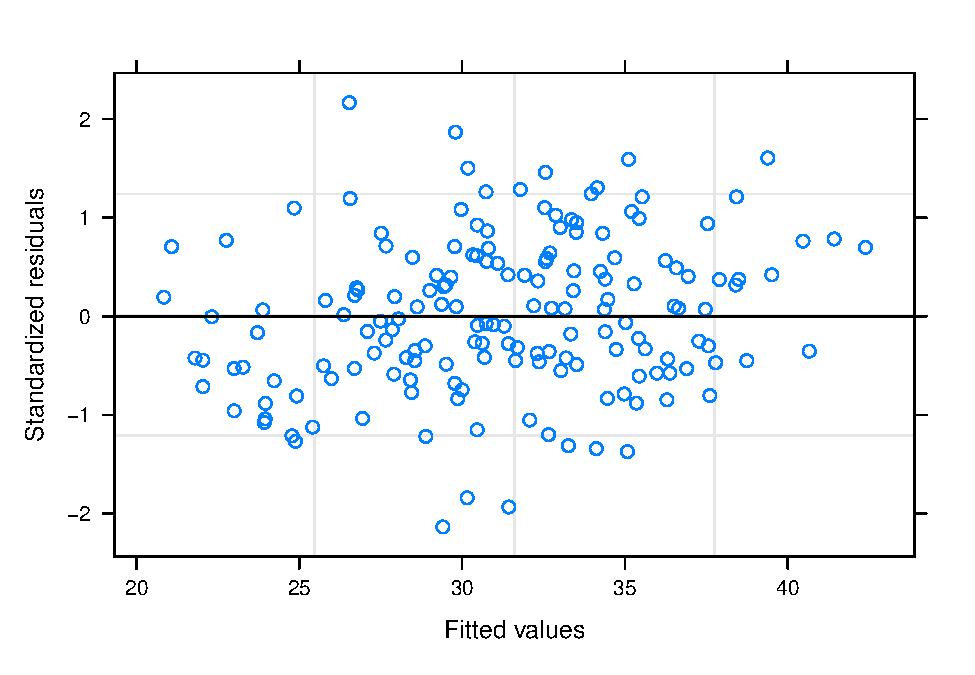
\includegraphics{fig_out/unnamed-chunk-129-1.pdf}

\begin{Shaded}
\begin{Highlighting}[]
\FunctionTok{qqnorm}\NormalTok{(modelo)}
\end{Highlighting}
\end{Shaded}

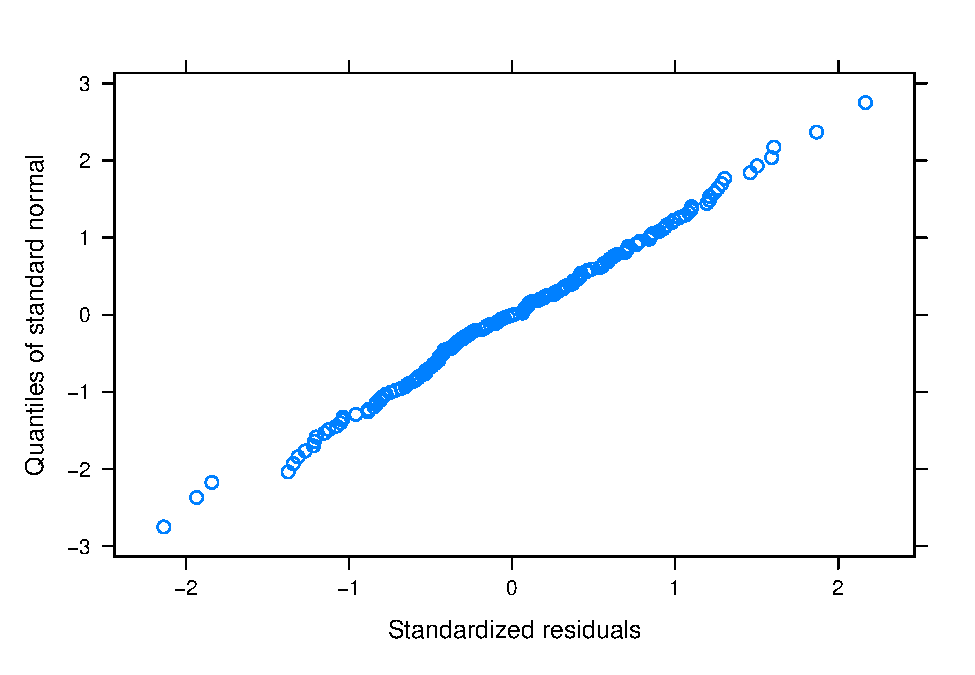
\includegraphics{fig_out/unnamed-chunk-129-2.pdf}

\begin{itemize}
\tightlist
\item
  Efectos aleatorios
\end{itemize}

\begin{Shaded}
\begin{Highlighting}[]
\NormalTok{beta0i}\OtherTok{\textless{}{-}} \FunctionTok{ranef}\NormalTok{(modelo)[,}\DecValTok{1}\NormalTok{]}
\FunctionTok{qqnorm}\NormalTok{(beta0i); }\FunctionTok{qqline}\NormalTok{(beta0i)}
\end{Highlighting}
\end{Shaded}

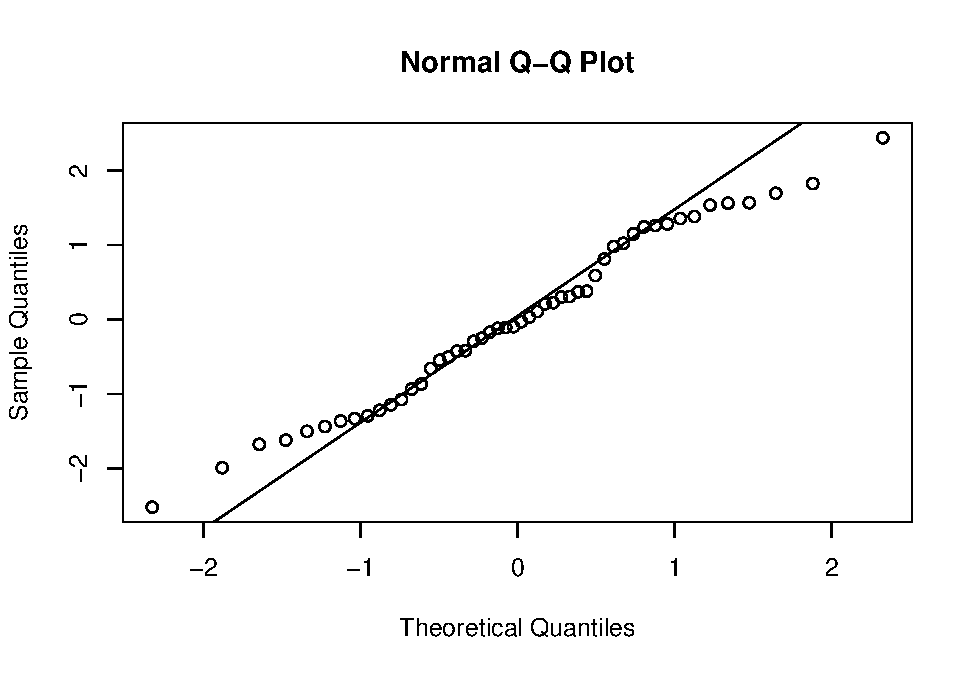
\includegraphics{fig_out/unnamed-chunk-130-1.pdf}

\begin{Shaded}
\begin{Highlighting}[]
\NormalTok{edad }\OtherTok{\textless{}{-}} \FunctionTok{with}\NormalTok{(datos, }\FunctionTok{tapply}\NormalTok{(edad, indiv, mean))}
\CommentTok{\# gráfico de los efectos aleatorios vs variables individuo}
\FunctionTok{plot}\NormalTok{(edad, beta0i)}
\end{Highlighting}
\end{Shaded}

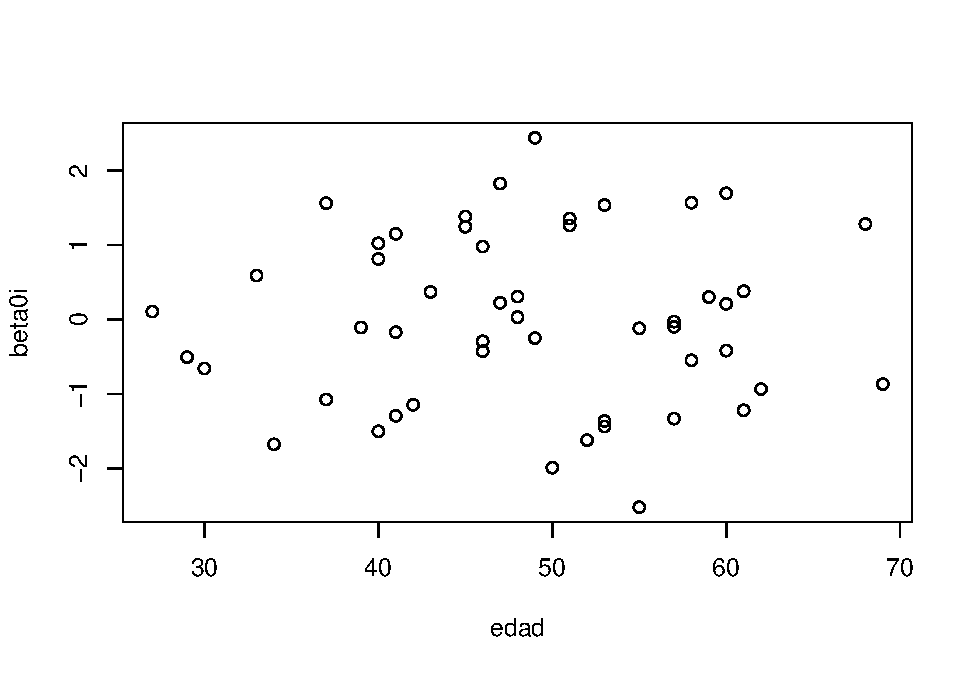
\includegraphics{fig_out/unnamed-chunk-130-2.pdf}

Parece que los efectos aleatorios siguen una distribución normal. Y no están relacionados con la edad.

\textbf{Predicciones}

\begin{Shaded}
\begin{Highlighting}[]
\FunctionTok{library}\NormalTok{(ggeffects)}
\NormalTok{pr }\OtherTok{\textless{}{-}} \FunctionTok{ggpredict}\NormalTok{(modelo, }\AttributeTok{terms =} \FunctionTok{c}\NormalTok{(}\StringTok{"tiempo [all]"}\NormalTok{))}
\NormalTok{pr}
\end{Highlighting}
\end{Shaded}

\begin{verbatim}
# Predicted values of respuesta

tiempo | Predicted |         95% CI
-----------------------------------
     0 |     32.57 | [31.89, 33.25]
     1 |     31.61 | [30.99, 32.24]
     2 |     30.65 | [30.02, 31.28]
     3 |     29.69 | [29.00, 30.38]

Adjusted for:
*  edad = 48.00
* indiv = 26.00
\end{verbatim}

\begin{Shaded}
\begin{Highlighting}[]
\FunctionTok{plot}\NormalTok{(pr, }\AttributeTok{add.data =} \ConstantTok{TRUE}\NormalTok{)}
\end{Highlighting}
\end{Shaded}

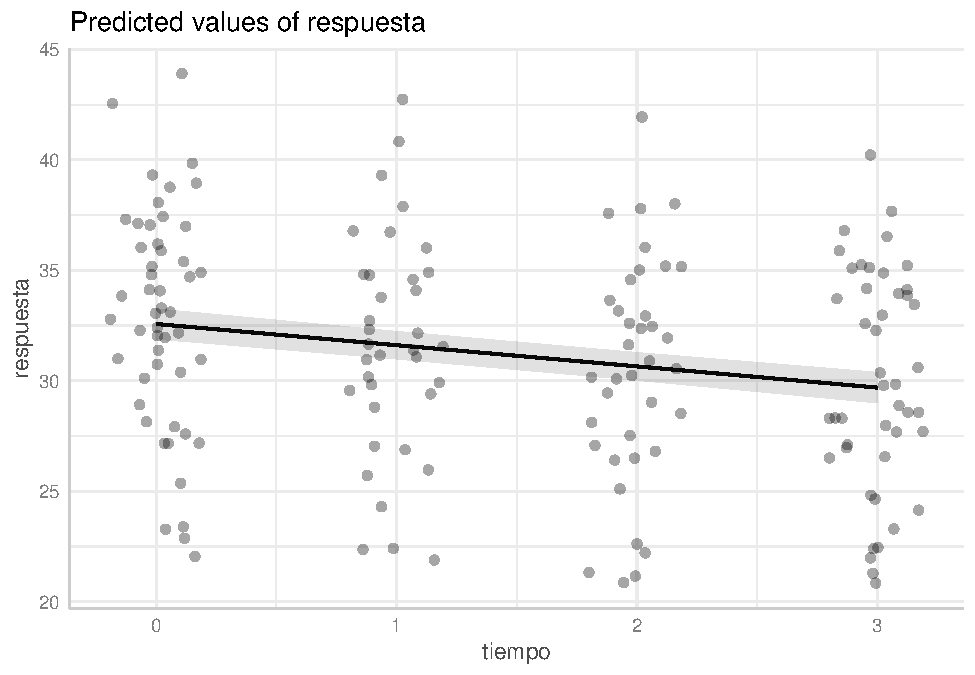
\includegraphics{fig_out/unnamed-chunk-131-1.pdf}

\begin{Shaded}
\begin{Highlighting}[]
\FunctionTok{plot}\NormalTok{(pr, }\AttributeTok{residuals =} \ConstantTok{TRUE}\NormalTok{)}
\end{Highlighting}
\end{Shaded}

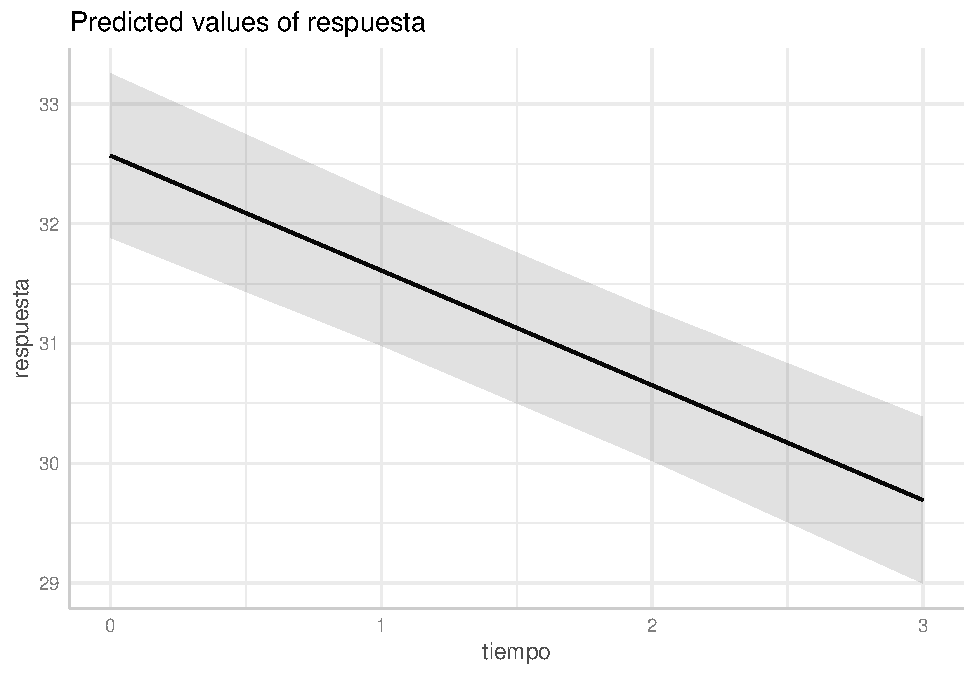
\includegraphics{fig_out/unnamed-chunk-131-2.pdf}

Las predicciones las realiza en la media de las covariables, en este caso la edad.
Si queremos que las predicciones las haga para un individuo de 55 años:

\begin{Shaded}
\begin{Highlighting}[]
\NormalTok{pr }\OtherTok{\textless{}{-}} \FunctionTok{ggpredict}\NormalTok{(modelo, }\AttributeTok{terms =} \FunctionTok{c}\NormalTok{(}\StringTok{"tiempo [all]"}\NormalTok{), }\AttributeTok{condition=}\FunctionTok{c}\NormalTok{(}\StringTok{"edad"}\OtherTok{=}\DecValTok{55}\NormalTok{))}
\NormalTok{pr}
\end{Highlighting}
\end{Shaded}

\begin{verbatim}
# Predicted values of respuesta

tiempo | Predicted |         95% CI
-----------------------------------
     0 |     35.56 | [34.76, 36.35]
     1 |     34.60 | [33.86, 35.34]
     2 |     33.64 | [32.89, 34.38]
     3 |     32.68 | [31.88, 33.48]

Adjusted for:
* indiv = 26.00
\end{verbatim}

\begin{Shaded}
\begin{Highlighting}[]
\FunctionTok{plot}\NormalTok{(pr)}
\end{Highlighting}
\end{Shaded}

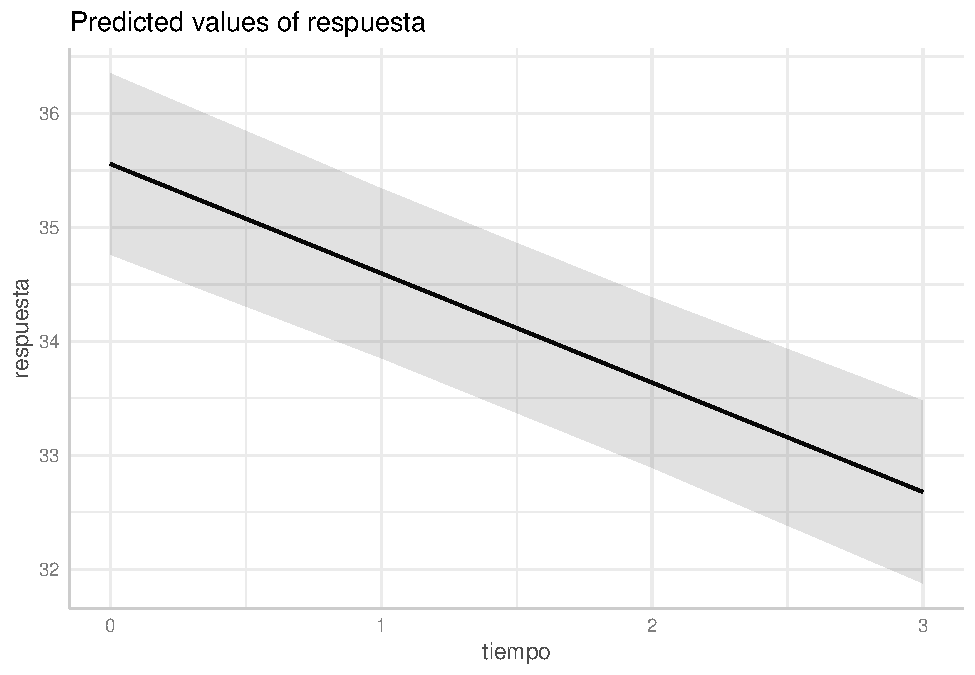
\includegraphics{fig_out/unnamed-chunk-132-1.pdf}

\hypertarget{comparaciuxf3n-de-los-dos-tratamientos}{%
\subsubsection{Comparación de los dos tratamientos}\label{comparaciuxf3n-de-los-dos-tratamientos}}

\begin{Shaded}
\begin{Highlighting}[]
\NormalTok{datos }\OtherTok{\textless{}{-}} \FunctionTok{read.csv2}\NormalTok{(}\StringTok{"datos/imc.csv"}\NormalTok{)}
\NormalTok{datos }\OtherTok{\textless{}{-}}\NormalTok{ datos[}\FunctionTok{order}\NormalTok{(datos}\SpecialCharTok{$}\NormalTok{indiv,datos}\SpecialCharTok{$}\NormalTok{tiempo),]}
\NormalTok{datos }\OtherTok{\textless{}{-}} \FunctionTok{na.omit}\NormalTok{(datos) }\CommentTok{\# para eliminar datos con missings (pero no individuos)}
\end{Highlighting}
\end{Shaded}

Volvemos al enunciado original trabajando con todos los datos. Ahora el objetivo es comparar la evolución de los dos tratamientos ajustando por la edad.

\begin{Shaded}
\begin{Highlighting}[]
\FunctionTok{library}\NormalTok{(nlme)}
\NormalTok{modelo }\OtherTok{\textless{}{-}} \FunctionTok{lme}\NormalTok{(respuesta }\SpecialCharTok{\textasciitilde{}} \FunctionTok{poly}\NormalTok{(tiempo, }\DecValTok{3}\NormalTok{, }\AttributeTok{raw=}\DecValTok{3}\NormalTok{) }\SpecialCharTok{+}\NormalTok{ tx}\SpecialCharTok{:}\FunctionTok{poly}\NormalTok{(tiempo, }\DecValTok{3}\NormalTok{, }\AttributeTok{raw=}\DecValTok{3}\NormalTok{) }\SpecialCharTok{+}\NormalTok{ edad,}
              \AttributeTok{random=} \SpecialCharTok{\textasciitilde{}} \FunctionTok{poly}\NormalTok{(tiempo, }\DecValTok{3}\NormalTok{, }\AttributeTok{raw=}\DecValTok{3}\NormalTok{)  }\SpecialCharTok{|}\NormalTok{ indiv, }
              \AttributeTok{data=}\NormalTok{datos, }
              \AttributeTok{correlation=}\FunctionTok{corCAR1}\NormalTok{(}\AttributeTok{form =} \SpecialCharTok{\textasciitilde{}}\NormalTok{ tiempo}\SpecialCharTok{|}\NormalTok{indiv))}
\FunctionTok{summary}\NormalTok{(modelo)}
\end{Highlighting}
\end{Shaded}

\begin{verbatim}
Linear mixed-effects model fit by REML
  Data: datos 
       AIC     BIC    logLik
  1417.874 1494.57 -688.9369

Random effects:
 Formula: ~poly(tiempo, 3, raw = 3) | indiv
 Structure: General positive-definite, Log-Cholesky parametrization
                          StdDev    Corr  
(Intercept)               2.3069274 (Intr)
poly(tiempo, 3, raw = 3)1 1.9231468 -0.470
poly(tiempo, 3, raw = 3)2 1.7013762  0.354
poly(tiempo, 3, raw = 3)3 0.3562430 -0.342
Residual                  0.9432126       
                                               
(Intercept)               p(,3,r=3)1 p(,3,r=3)2
poly(tiempo, 3, raw = 3)1                      
poly(tiempo, 3, raw = 3)2 -0.904               
poly(tiempo, 3, raw = 3)3  0.852     -0.990    
Residual                                       

Correlation Structure: Continuous AR(1)
 Formula: ~tiempo | indiv 
 Parameter estimate(s):
     Phi 
0.248855 
Fixed effects:  respuesta ~ poly(tiempo, 3, raw = 3) + tx:poly(tiempo, 3, raw = 3) +      edad 
                                 Value Std.Error
(Intercept)                  11.168714 1.1301845
poly(tiempo, 3, raw = 3)1     2.402332 1.2555058
poly(tiempo, 3, raw = 3)2    -2.075890 1.1602056
poly(tiempo, 3, raw = 3)3     0.447207 0.2546185
edad                          0.442918 0.0224834
poly(tiempo, 3, raw = 3)1:tx -2.107063 0.7636948
poly(tiempo, 3, raw = 3)2:tx  0.905552 0.7097238
poly(tiempo, 3, raw = 3)3:tx -0.194165 0.1561157
                              DF   t-value
(Intercept)                  244  9.882204
poly(tiempo, 3, raw = 3)1    244  1.913438
poly(tiempo, 3, raw = 3)2    244 -1.789243
poly(tiempo, 3, raw = 3)3    244  1.756379
edad                          98 19.699782
poly(tiempo, 3, raw = 3)1:tx 244 -2.759037
poly(tiempo, 3, raw = 3)2:tx 244  1.275922
poly(tiempo, 3, raw = 3)3:tx 244 -1.243724
                             p-value
(Intercept)                   0.0000
poly(tiempo, 3, raw = 3)1     0.0569
poly(tiempo, 3, raw = 3)2     0.0748
poly(tiempo, 3, raw = 3)3     0.0803
edad                          0.0000
poly(tiempo, 3, raw = 3)1:tx  0.0062
poly(tiempo, 3, raw = 3)2:tx  0.2032
poly(tiempo, 3, raw = 3)3:tx  0.2148
 Correlation: 
                             (Intr) pl(,3,r=3)1
poly(tiempo, 3, raw = 3)1    -0.048            
poly(tiempo, 3, raw = 3)2     0.033 -0.949     
poly(tiempo, 3, raw = 3)3    -0.028  0.899     
edad                         -0.975  0.027     
poly(tiempo, 3, raw = 3)1:tx  0.020 -0.948     
poly(tiempo, 3, raw = 3)2:tx -0.013  0.898     
poly(tiempo, 3, raw = 3)3:tx  0.010 -0.849     
                             pl(,3,r=3)2
poly(tiempo, 3, raw = 3)1               
poly(tiempo, 3, raw = 3)2               
poly(tiempo, 3, raw = 3)3    -0.989     
edad                         -0.020     
poly(tiempo, 3, raw = 3)1:tx  0.903     
poly(tiempo, 3, raw = 3)2:tx -0.951     
poly(tiempo, 3, raw = 3)3:tx  0.939     
                             pl(,3,r=3)3 edad  
poly(tiempo, 3, raw = 3)1                      
poly(tiempo, 3, raw = 3)2                      
poly(tiempo, 3, raw = 3)3                      
edad                          0.016            
poly(tiempo, 3, raw = 3)1:tx -0.856      -0.020
poly(tiempo, 3, raw = 3)2:tx  0.941       0.013
poly(tiempo, 3, raw = 3)3:tx -0.951      -0.010
                             p(,3,r=3)1:
poly(tiempo, 3, raw = 3)1               
poly(tiempo, 3, raw = 3)2               
poly(tiempo, 3, raw = 3)3               
edad                                    
poly(tiempo, 3, raw = 3)1:tx            
poly(tiempo, 3, raw = 3)2:tx -0.947     
poly(tiempo, 3, raw = 3)3:tx  0.896     
                             p(,3,r=3)2:
poly(tiempo, 3, raw = 3)1               
poly(tiempo, 3, raw = 3)2               
poly(tiempo, 3, raw = 3)3               
edad                                    
poly(tiempo, 3, raw = 3)1:tx            
poly(tiempo, 3, raw = 3)2:tx            
poly(tiempo, 3, raw = 3)3:tx -0.988     

Standardized Within-Group Residuals:
        Min          Q1         Med          Q3 
-1.65153170 -0.36449401 -0.04684107  0.39784060 
        Max 
 1.80027927 

Number of Observations: 350
Number of Groups: 100 
\end{verbatim}

Nota: \texttt{poly(tiempo,\ 3,\ raw=TRUE)} es lo miso que \texttt{tiempo\ +\ I(tiempo\^{}2)\ +\ I(tiempo\^{}3)}.

Fijate cómo se ha escrito la fórmula. De esta manera, cuando tiempo=0 (momento basal) no hay diferencias entre en los tratamientos.

\textbf{Efectos aleatorios}

\begin{Shaded}
\begin{Highlighting}[]
\FunctionTok{anova}\NormalTok{(modelo, }\FunctionTok{update}\NormalTok{(modelo, }\AttributeTok{random =} \SpecialCharTok{\textasciitilde{}} \DecValTok{1} \SpecialCharTok{|}\NormalTok{ indiv))}
\end{Highlighting}
\end{Shaded}

\begin{verbatim}
                                    Model df
modelo                                  1 20
update(modelo, random = ~1 | indiv)     2 11
                                         AIC
modelo                              1417.874
update(modelo, random = ~1 | indiv) 1408.597
                                        BIC
modelo                              1494.57
update(modelo, random = ~1 | indiv) 1450.78
                                       logLik
modelo                              -688.9369
update(modelo, random = ~1 | indiv) -693.2985
                                      Test
modelo                                    
update(modelo, random = ~1 | indiv) 1 vs 2
                                    L.Ratio
modelo                                     
update(modelo, random = ~1 | indiv)  8.7233
                                    p-value
modelo                                     
update(modelo, random = ~1 | indiv)  0.4632
\end{verbatim}

Vemos en este caso, como el p-valor del LRT no coincide con la decisión basada en el AIC o el BIC. Podemos decantarnos con el modelo más simple, o sea, el que supone que los coeficientes del tiempo son fijos.

\begin{Shaded}
\begin{Highlighting}[]
\NormalTok{modelo }\OtherTok{\textless{}{-}} \FunctionTok{update}\NormalTok{(modelo, }\AttributeTok{random =} \SpecialCharTok{\textasciitilde{}} \DecValTok{1} \SpecialCharTok{|}\NormalTok{ indiv)}
\end{Highlighting}
\end{Shaded}

\textbf{Estructura de correlación de los errores}

Comparamos con la matriz de independencia

\begin{Shaded}
\begin{Highlighting}[]
\FunctionTok{anova}\NormalTok{(modelo, }\FunctionTok{update}\NormalTok{(modelo, }\AttributeTok{correlation=}\ConstantTok{NULL}\NormalTok{))}
\end{Highlighting}
\end{Shaded}

\begin{verbatim}
                                   Model df
modelo                                 1 11
update(modelo, correlation = NULL)     2 10
                                        AIC
modelo                             1408.597
update(modelo, correlation = NULL) 1446.555
                                        BIC
modelo                             1450.780
update(modelo, correlation = NULL) 1484.903
                                      logLik
modelo                             -693.2985
update(modelo, correlation = NULL) -713.2774
                                     Test
modelo                                   
update(modelo, correlation = NULL) 1 vs 2
                                    L.Ratio
modelo                                     
update(modelo, correlation = NULL) 39.95779
                                   p-value
modelo                                    
update(modelo, correlation = NULL)  <.0001
\end{verbatim}

Nos quedamos con la estructura AR1.

Finalmente, comprovamos los efectos fijos:

\begin{Shaded}
\begin{Highlighting}[]
\FunctionTok{coef}\NormalTok{(}\FunctionTok{summary}\NormalTok{(modelo))}
\end{Highlighting}
\end{Shaded}

\begin{verbatim}
                                  Value
(Intercept)                  10.9983674
poly(tiempo, 3, raw = 3)1     2.2104398
poly(tiempo, 3, raw = 3)2    -1.8762381
poly(tiempo, 3, raw = 3)3     0.4026454
edad                          0.4463927
poly(tiempo, 3, raw = 3)1:tx -1.9653182
poly(tiempo, 3, raw = 3)2:tx  0.7598944
poly(tiempo, 3, raw = 3)3:tx -0.1617992
                              Std.Error  DF
(Intercept)                  1.17012354 244
poly(tiempo, 3, raw = 3)1    1.28087236 244
poly(tiempo, 3, raw = 3)2    1.14921815 244
poly(tiempo, 3, raw = 3)3    0.25308582 244
edad                         0.02329682  98
poly(tiempo, 3, raw = 3)1:tx 0.78262641 244
poly(tiempo, 3, raw = 3)2:tx 0.70301744 244
poly(tiempo, 3, raw = 3)3:tx 0.15513365 244
                               t-value
(Intercept)                   9.399322
poly(tiempo, 3, raw = 3)1     1.725730
poly(tiempo, 3, raw = 3)2    -1.632621
poly(tiempo, 3, raw = 3)3     1.590944
edad                         19.161101
poly(tiempo, 3, raw = 3)1:tx -2.511183
poly(tiempo, 3, raw = 3)2:tx  1.080904
poly(tiempo, 3, raw = 3)3:tx -1.042967
                                  p-value
(Intercept)                  4.150278e-18
poly(tiempo, 3, raw = 3)1    8.566199e-02
poly(tiempo, 3, raw = 3)2    1.038384e-01
poly(tiempo, 3, raw = 3)3    1.129169e-01
edad                         6.509723e-35
poly(tiempo, 3, raw = 3)1:tx 1.268004e-02
poly(tiempo, 3, raw = 3)2:tx 2.808070e-01
poly(tiempo, 3, raw = 3)3:tx 2.979960e-01
\end{verbatim}

Como era de esperar, la edad es muy significativa.

Contrastamos el efecto cuadrático y cúbico del tiempo (tanto para el grupo control como para el grupo de tratados):

\begin{Shaded}
\begin{Highlighting}[]
\NormalTok{modelo2 }\OtherTok{\textless{}{-}} \FunctionTok{update}\NormalTok{(modelo, }\AttributeTok{fixed =}\NormalTok{ . }\SpecialCharTok{\textasciitilde{}}\NormalTok{ tiempo }\SpecialCharTok{+}\NormalTok{ tiempo}\SpecialCharTok{:}\NormalTok{tx }\SpecialCharTok{+}\NormalTok{ edad)}
\FunctionTok{coef}\NormalTok{(}\FunctionTok{summary}\NormalTok{(modelo2))}
\end{Highlighting}
\end{Shaded}

\begin{verbatim}
                 Value  Std.Error  DF    t-value
(Intercept) 11.0143619 1.16920806 248  9.4203610
tiempo       0.1947449 0.21775844 248  0.8943163
edad         0.4462810 0.02328366  98 19.1671311
tiempo:tx   -1.1381679 0.13574697 248 -8.3844810
                 p-value
(Intercept) 3.281588e-18
tiempo      3.720198e-01
edad        6.352777e-35
tiempo:tx   3.860440e-15
\end{verbatim}

\begin{Shaded}
\begin{Highlighting}[]
\FunctionTok{anova}\NormalTok{(modelo, modelo2)}
\end{Highlighting}
\end{Shaded}

\begin{verbatim}
        Model df      AIC      BIC    logLik
modelo      1 11 1408.597 1450.780 -693.2985
modelo2     2  7 1394.327 1421.252 -690.1637
          Test  L.Ratio p-value
modelo                         
modelo2 1 vs 2 6.269749  0.1799
\end{verbatim}

Como el p-valor del LRT es \textgreater0.05, nos quedamos con el modelo más simple, en que el tiempo tiene un efecto lineal en ambos grupos

\begin{Shaded}
\begin{Highlighting}[]
\NormalTok{modelo }\OtherTok{\textless{}{-}}\NormalTok{ modelo2}
\FunctionTok{coef}\NormalTok{(}\FunctionTok{summary}\NormalTok{(modelo))}
\end{Highlighting}
\end{Shaded}

\begin{verbatim}
                 Value  Std.Error  DF    t-value
(Intercept) 11.0143619 1.16920806 248  9.4203610
tiempo       0.1947449 0.21775844 248  0.8943163
edad         0.4462810 0.02328366  98 19.1671311
tiempo:tx   -1.1381679 0.13574697 248 -8.3844810
                 p-value
(Intercept) 3.281588e-18
tiempo      3.720198e-01
edad        6.352777e-35
tiempo:tx   3.860440e-15
\end{verbatim}

El efecto del tiempo en el grupo control no es significativo.

Para ver el efecto del tiempo en el grupo de tratamiento, cambiamos la categoria de referencia:

\begin{Shaded}
\begin{Highlighting}[]
\NormalTok{datos}\SpecialCharTok{$}\NormalTok{tx }\OtherTok{\textless{}{-}} \FunctionTok{factor}\NormalTok{(datos}\SpecialCharTok{$}\NormalTok{tx, }\DecValTok{2}\SpecialCharTok{:}\DecValTok{1}\NormalTok{)}
\FunctionTok{coef}\NormalTok{(}\FunctionTok{summary}\NormalTok{(}\FunctionTok{update}\NormalTok{(modelo)))}
\end{Highlighting}
\end{Shaded}

\begin{verbatim}
                Value  Std.Error  DF    t-value
(Intercept) 11.014362 1.16920806 248   9.420361
tiempo      -2.081591 0.10101027 248 -20.607715
edad         0.446281 0.02328366  98  19.167131
tiempo:tx1   1.138168 0.13574697 248   8.384481
                 p-value
(Intercept) 3.281588e-18
tiempo      1.166972e-55
edad        6.352777e-35
tiempo:tx1  3.860440e-15
\end{verbatim}

Vemos como el efecto del tiempo en el grupo de tratados es significativo y la pendiente es negativa.

\textbf{Validación}

\begin{Shaded}
\begin{Highlighting}[]
\CommentTok{\# residuos}
\FunctionTok{plot}\NormalTok{(modelo)}
\end{Highlighting}
\end{Shaded}

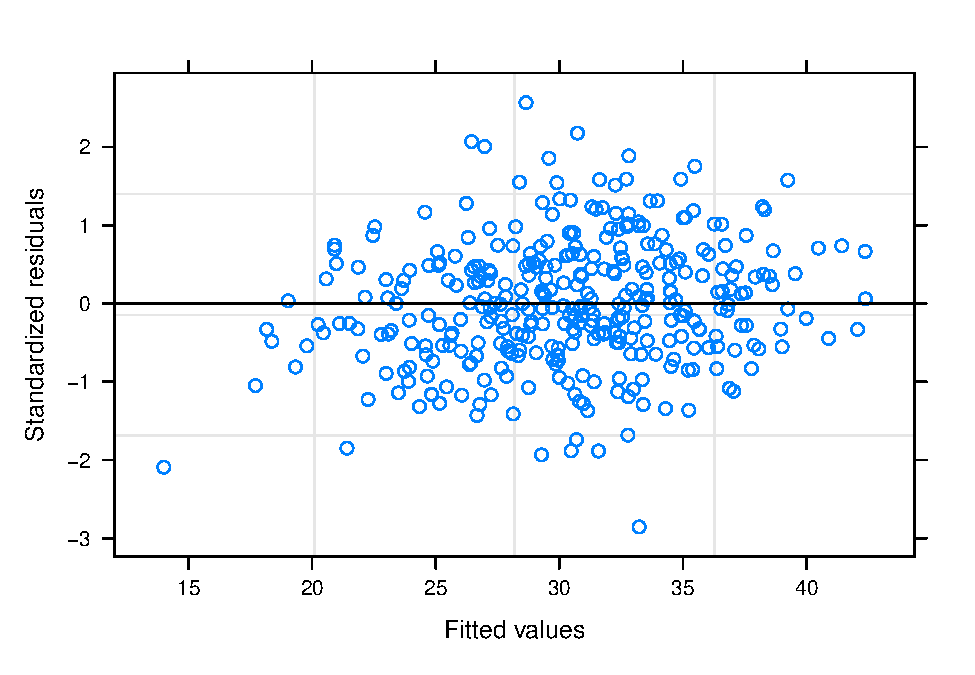
\includegraphics{fig_out/unnamed-chunk-142-1.pdf}

\begin{Shaded}
\begin{Highlighting}[]
\FunctionTok{qqnorm}\NormalTok{(modelo)}
\end{Highlighting}
\end{Shaded}

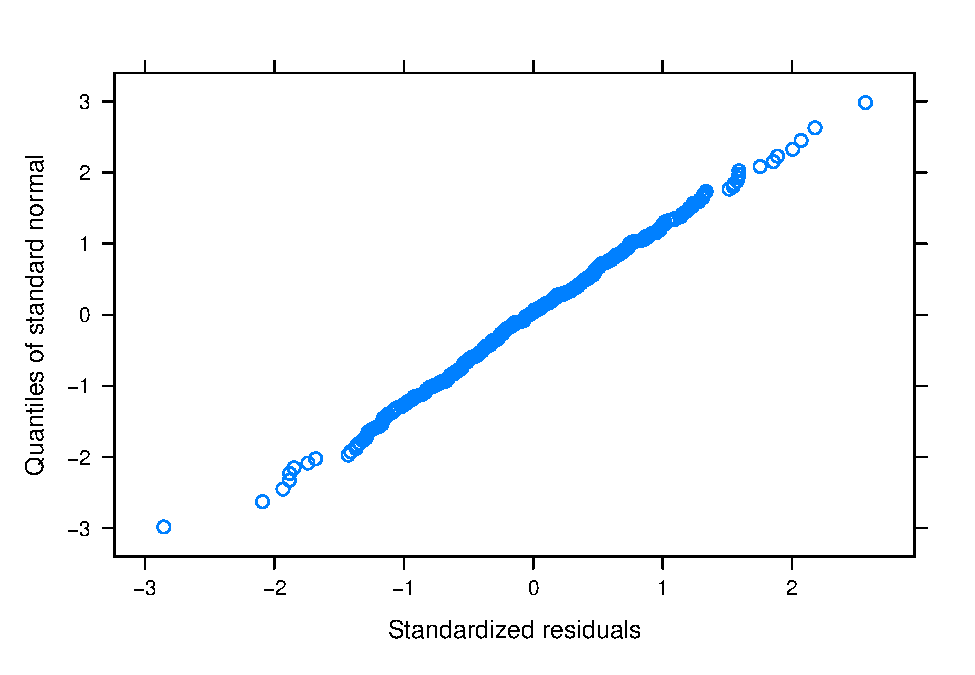
\includegraphics{fig_out/unnamed-chunk-142-2.pdf}

\begin{Shaded}
\begin{Highlighting}[]
\CommentTok{\# efectos aleatorios}
\NormalTok{beta0i }\OtherTok{\textless{}{-}} \FunctionTok{ranef}\NormalTok{(modelo)[,}\DecValTok{1}\NormalTok{]}
\NormalTok{grupo }\OtherTok{\textless{}{-}} \FunctionTok{with}\NormalTok{(datos, }\FunctionTok{tapply}\NormalTok{(tx, indiv, head, }\AttributeTok{n=}\DecValTok{1}\NormalTok{))}
\NormalTok{edad }\OtherTok{\textless{}{-}} \FunctionTok{with}\NormalTok{(datos, }\FunctionTok{tapply}\NormalTok{(edad, indiv, mean))}
\FunctionTok{boxplot}\NormalTok{(beta0i }\SpecialCharTok{\textasciitilde{}}\NormalTok{ grupo)}
\end{Highlighting}
\end{Shaded}

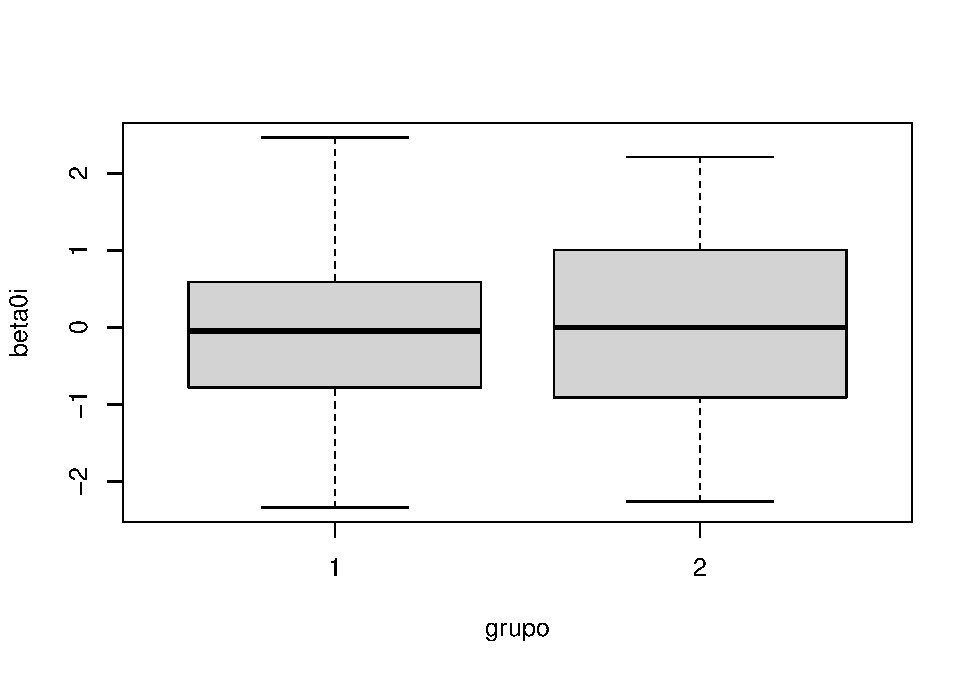
\includegraphics{fig_out/unnamed-chunk-142-3.pdf}

\begin{Shaded}
\begin{Highlighting}[]
\FunctionTok{plot}\NormalTok{(edad, beta0i)}
\end{Highlighting}
\end{Shaded}

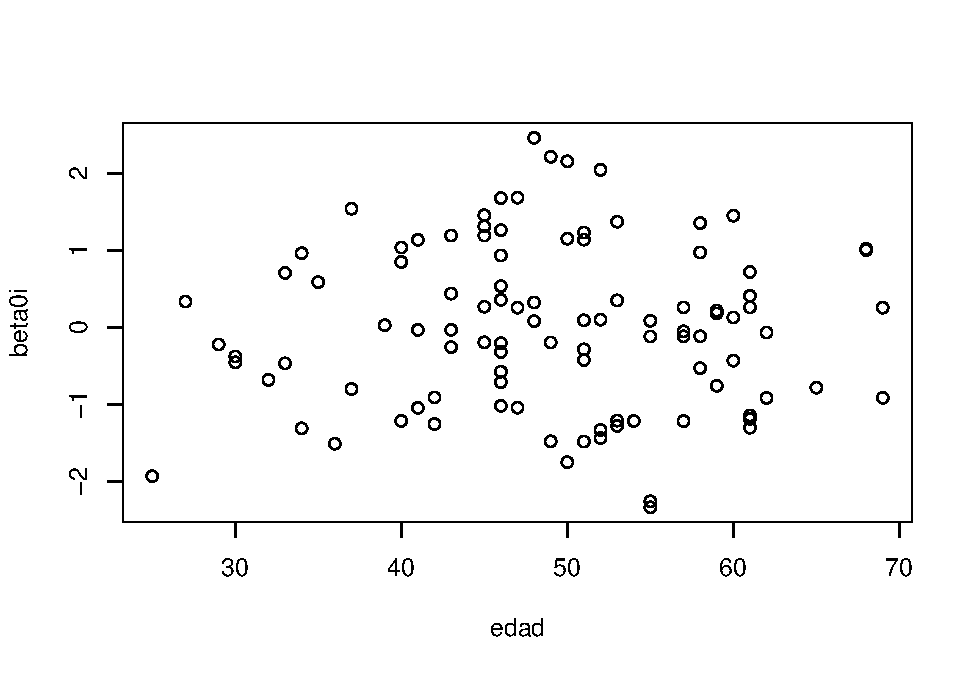
\includegraphics{fig_out/unnamed-chunk-142-4.pdf}

\textbf{Predicciones}

\begin{Shaded}
\begin{Highlighting}[]
\NormalTok{datos}\SpecialCharTok{$}\NormalTok{tx }\OtherTok{\textless{}{-}} \FunctionTok{factor}\NormalTok{(datos}\SpecialCharTok{$}\NormalTok{tx, }\DecValTok{1}\SpecialCharTok{:}\DecValTok{2}\NormalTok{)}
\NormalTok{modelo }\OtherTok{\textless{}{-}} \FunctionTok{update}\NormalTok{(modelo)}

\NormalTok{pr.cont }\OtherTok{\textless{}{-}} \FunctionTok{ggpredict}\NormalTok{(modelo, }\AttributeTok{terms =} \FunctionTok{c}\NormalTok{(}\StringTok{"tiempo"}\NormalTok{), }\AttributeTok{condition=}\FunctionTok{c}\NormalTok{(}\AttributeTok{tx=}\DecValTok{1}\NormalTok{), }\AttributeTok{type=}\StringTok{"fixed"}\NormalTok{)}
\NormalTok{pr.tx }\OtherTok{\textless{}{-}} \FunctionTok{ggpredict}\NormalTok{(modelo, }\AttributeTok{terms =} \FunctionTok{c}\NormalTok{(}\StringTok{"tiempo"}\NormalTok{), }\AttributeTok{condition=}\FunctionTok{c}\NormalTok{(}\AttributeTok{tx=}\DecValTok{2}\NormalTok{), }\AttributeTok{type=}\StringTok{"fixed"}\NormalTok{)}
\NormalTok{pr.cont}
\end{Highlighting}
\end{Shaded}

\begin{verbatim}
# Predicted values of respuesta

tiempo | Predicted |         95% CI
-----------------------------------
     0 |     32.88 | [32.39, 33.38]
     1 |     31.94 | [31.47, 32.41]
     2 |     31.00 | [30.47, 31.52]
     3 |     30.05 | [29.41, 30.69]

Adjusted for:
*  edad = 49.00
* indiv = 52.50
\end{verbatim}

\begin{Shaded}
\begin{Highlighting}[]
\NormalTok{pr.tx}
\end{Highlighting}
\end{Shaded}

\begin{verbatim}
# Predicted values of respuesta

tiempo | Predicted |         95% CI
-----------------------------------
     0 |     32.88 | [32.39, 33.38]
     1 |     30.80 | [30.33, 31.27]
     2 |     28.72 | [28.19, 29.25]
     3 |     26.64 | [25.99, 27.28]

Adjusted for:
*  edad = 49.00
* indiv = 52.50
\end{verbatim}

\begin{Shaded}
\begin{Highlighting}[]
\FunctionTok{library}\NormalTok{(gridExtra)}
\FunctionTok{grid.arrange}\NormalTok{(}
    \FunctionTok{plot}\NormalTok{(pr.cont) }\SpecialCharTok{+} \FunctionTok{ylim}\NormalTok{(}\DecValTok{24}\NormalTok{,}\DecValTok{40}\NormalTok{) }\SpecialCharTok{+} \FunctionTok{ggtitle}\NormalTok{(}\StringTok{"controles"}\NormalTok{),}
    \FunctionTok{plot}\NormalTok{(pr.tx) }\SpecialCharTok{+} \FunctionTok{ylim}\NormalTok{(}\DecValTok{24}\NormalTok{,}\DecValTok{40}\NormalTok{) }\SpecialCharTok{+} \FunctionTok{ggtitle}\NormalTok{(}\StringTok{"tratados"}\NormalTok{),}
\AttributeTok{nrow=}\DecValTok{1}\NormalTok{, }\AttributeTok{ncol=}\DecValTok{2}\NormalTok{)}
\end{Highlighting}
\end{Shaded}

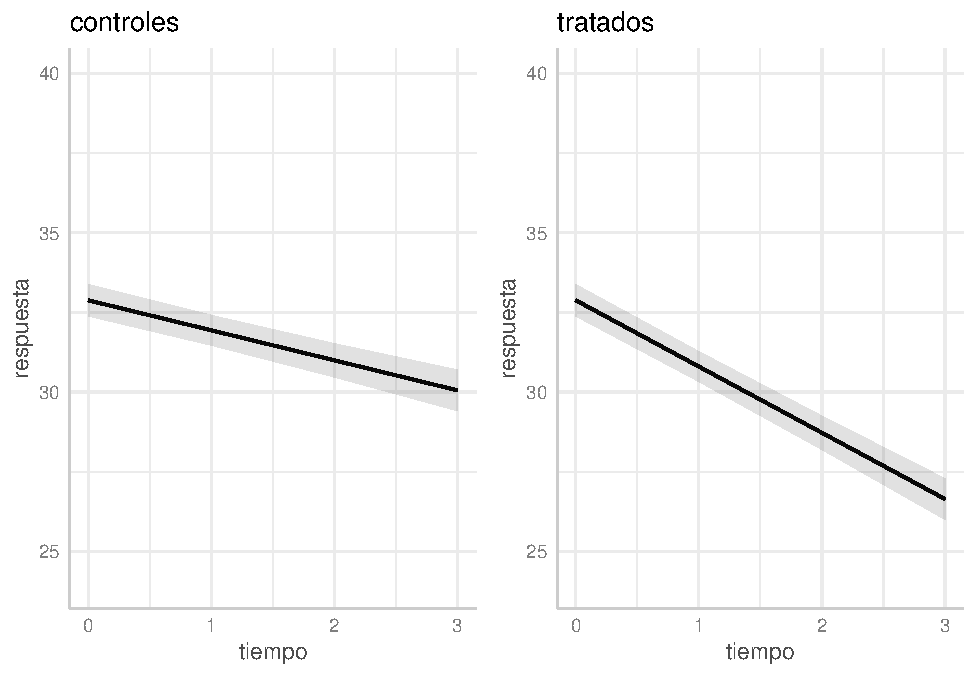
\includegraphics{fig_out/unnamed-chunk-143-1.pdf}

\hypertarget{ejercicios-1}{%
\section{Ejercicios}\label{ejercicios-1}}

\hypertarget{ejercicio-4}{%
\subsection{Ejercicio 4}\label{ejercicio-4}}

\begin{quote}
Los datos \texttt{sleepstudy} de la librería \texttt{lme4} contienen información sobre 18 dindividuos que se han seguido durante 9 días, y para los cuales se ha registrado el tiempo de reacción (en milisegundos) tras haber estado en deprivación de sueño.

Los datos pueden cargarse mediante
\end{quote}

\begin{Shaded}
\begin{Highlighting}[]
\FunctionTok{library}\NormalTok{(lme4)}
\FunctionTok{data}\NormalTok{(sleepstudy)}
\end{Highlighting}
\end{Shaded}

\begin{quote}
\begin{enumerate}
\def\labelenumi{\arabic{enumi}.}
\tightlist
\item
  Crea un spaguetti plot para ver la evolución de la reacción a lo largo del tiempo
\item
  Modeliza el tiempo de reacción (variable respuesta) a lo largo de los días. Usa tanto polinomios como splines con la función \texttt{ns()}. Puedes usar la función \texttt{anova()} con el test LRT para contrastar si es necesario usar términos splines (\texttt{ns()}) o polinomios \texttt{poly()}).
\end{enumerate}
\end{quote}

\hypertarget{ejercicio-5}{%
\subsection{Ejercicio 5}\label{ejercicio-5}}

\begin{quote}
Los datos \texttt{dietox} de la librería \texttt{geepack} contienen el peso de cerdos medidos semanalmente durante 12 semanas cuando son sacrificados (Weight). Los datos también contienen el peso en la semana 1 (Start), tres niveles diferentes de vitamina E (Evit - dosis: 0, 100, 200 mg dl-alfa-tocoferil acetato / kg de alimento) en combinación con 3 niveles diferentes de cobre (Cu - dosis: 0, 35, 175 mg / kg de alimento) que reciben en el alimento. También se registra la ingesta acumulada de alimento (Feed). Los cerdos son compañeros de camada (Litter). El objetivo principal es ver qué combinación de suplementos en el alimento hace que los cerdos alcancen un mayor peso.

\begin{enumerate}
\def\labelenumi{\arabic{enumi}.}
\tightlist
\item
  Haz una descriptiva de las variables (summary)
\item
  ¿Qué variables son tiempo dependientes y cuáles no? (crea un gráfico para Weight, Evit y Cu)
\item
  Ajusta un modelo mixto para contestar a la pregunta científica
\item
  ¿Qué variables as considerado con efecto aleatorio?
\item
  ¿Qué estructura de correlaciones has considerado?
\item
  Intenta cambiar algunos aspectos del modelo (añadir quitar coeficientes aleatorios, estructura de correlación de los errores, simplificar o añadir variables/interacciones, \ldots) para elegir el mejor modelo
\item
  Una vez escogido el modelo final, haz un gráfico de la evolución de la variable respuesta a diferentes niveles de \texttt{Start}.
\end{enumerate}
\end{quote}

\hypertarget{anuxe1lisis-de-supervivencia-con-datos-longitudinales}{%
\chapter{Análisis de supervivencia con datos longitudinales}\label{anuxe1lisis-de-supervivencia-con-datos-longitudinales}}

\hypertarget{tiempo-hasta-evento}{%
\section{Tiempo hasta evento}\label{tiempo-hasta-evento}}

En el análisis de superviviencia la variable respuesta es el \textbf{tiempo} hasta el evento de interés.

Normalente los datos se obtienen de un estudio de cohorte con seguimiento ya sea prospectivo o retrospectivo. Transcurrido el periodo de seguimiento o ``follow-up time'' puede que para alguno de los individuos de la muestra el evento de interés no se haya observado, ya sea porque ha finalizado el seguimiento o porque se han perdido o han tenido un evento diferente del de interés que ha interrumpido su seguimiento. En estos casos se suele decir que dichos individuos están \textbf{censurados}.

Es muy importante registrar el tiempo que ha pasado des del inicio hasta el evento para los no censurados y también el momento que se ha perdido el seguimiento para los censurados. Así hay que definir bien el momento de inicio y el momento final para cada participante del estudio. Y también es importante que el \textbf{mecanimso usado para obtener la información del seguimiento sea el mismo para todos.}

En la siguiente figura tenemos una descripción de cómo recogeríamos la información para diez individuos donde se observa que cada uno de ellos puede entrar en un momento distinto en el tiempo a partir del inicio del estudio (01/0108), que algunos se observa el evento de interés (puntos negros) y para otros el tiempo está censurado (puntos rojos) bien sea porque se acaba el periodo de seguimiento (01/01/2020) o porque abandonan el estudio antes del final (puntos rojos antes del 01/01/2020)

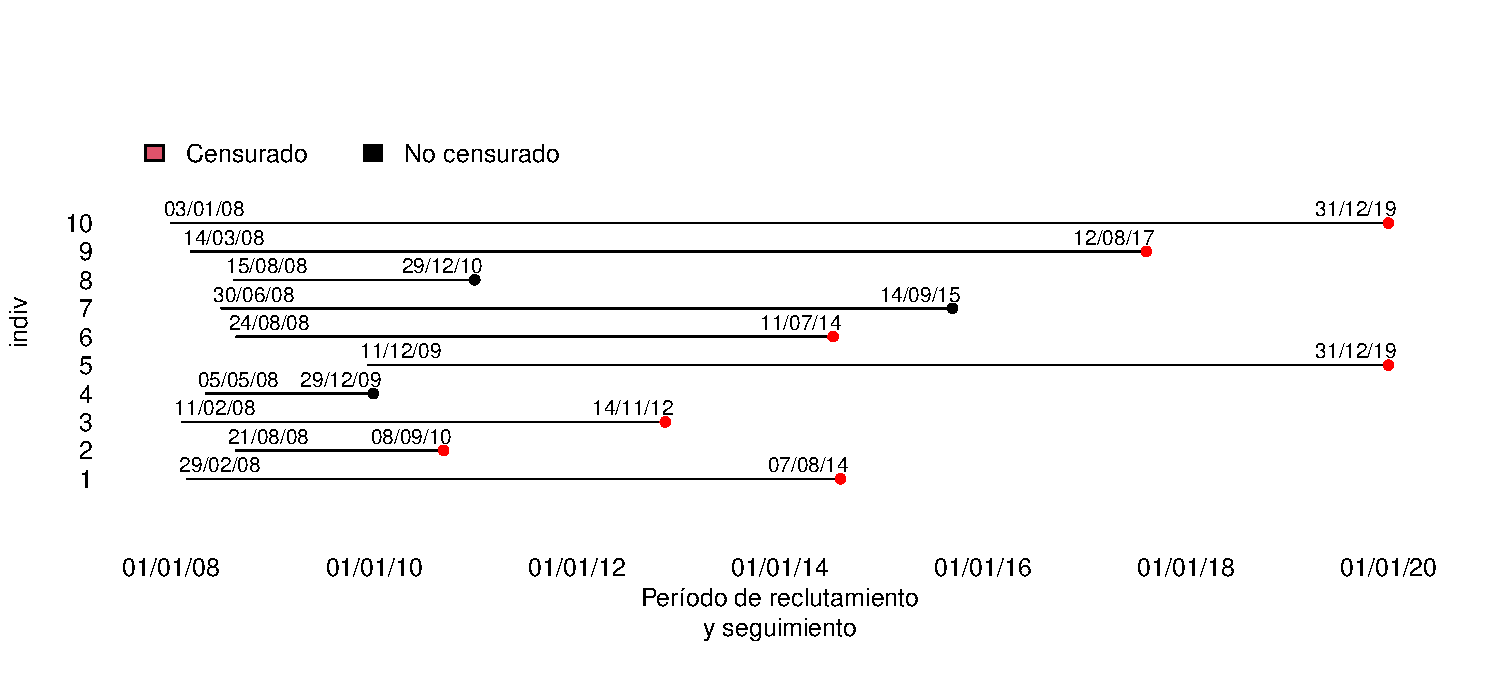
\includegraphics{fig_out/unnamed-chunk-145-1.pdf}

Normalment lo que hacemos es calcular el tiempo pasando toda la información a ``tiempo cero''. La siguiente figura muestra cómo quedarían los datos para el ejemplo anterior

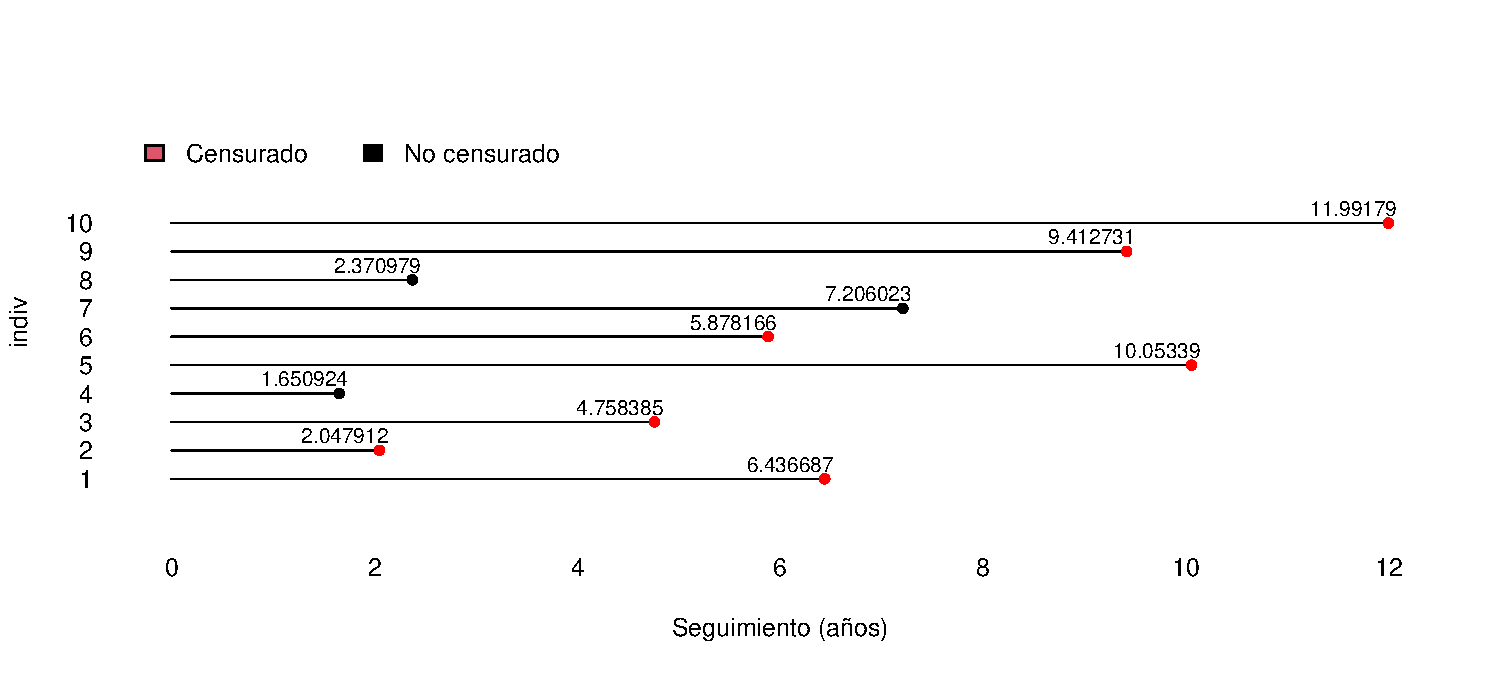
\includegraphics{fig_out/unnamed-chunk-146-1.pdf}

De esta forma, para cada individuo anotaríamos la variable tiempo y crearíamos otra variable 0/1 que sería 0 para aquellos individuos censurados (puntos rojos) y 1 para los que observamos el evento de interés (puntos negros). En la práctica no se habla de variable censurada, si no de la variable evento, y es por eso que codificamos 0 a la censura y 1 a aquellos casos en los que observamos nuestro evento de interés.

\hypertarget{ejemplos-3}{%
\subsection{Ejemplos}\label{ejemplos-3}}

\begin{quote}
Pacientes diagnosticados de cancer de próstata. Seguimiento hasta recidiva o muerte.
El inicio sería la fecha del diagnóstico y la fecha final sería la fechad e recidiva o muerte (para los no censurados) y la fecha de final de seguimiento para los censurados.
\end{quote}

\begin{quote}
Estudio de una cohorte prospectiva a 10 años para estudiar el riesgo de infarto agudo de miocardio incidente. La fecha de inicio sería la fecha de inclusión en el estudio, y la fecha final sería la fecha de ingreso por infarto o muerte por infarto (para los no censurados), y la fecha de final de seguimiento o fecha de muerte por otra causa (para los censurados).
\end{quote}

\hypertarget{otros-tipos-de-censura}{%
\subsection{Otros tipos de censura}\label{otros-tipos-de-censura}}

La censura que se ha descrito es concretamente censura por la derecha. Esto quiere decir que cuando un dato está censurado significa que és superior al tiempo observado.

Existen otros tipo de censura que no estudiaremos:

\begin{itemize}
\item
  Censura por la izquierda: el tiempo es menor que el observado.
\item
  Censura por intervalo: el tiempo se encuentra entre dos fechas o momentos determinados.
\item
  Truncamiento por la izquierda: en realidad no es una censura, sino que es un retraso en el inicio del seguimiento. O sea, que el individuo lleva un tiempo en riesgo pero que ha entrado más tarde en el estudio.
\end{itemize}

\hypertarget{kaplan-meier}{%
\section{Kaplan-Meier}\label{kaplan-meier}}

El método de Kaplan-Meier se usa para estimar la supervivencia o su complementario, la probabilidad de que el evento ocurra antes del tiempo \(t\).

Si no hubieran eventos censurados antes del tiempo \(t\), la probabilidad de que ocurra el evento en este periodo es simplemente \(d_t/n\) donde \(d_t\) es el númerod e eventos antes de \(t\) y \(n\) el número de individuos de la cohorte. Pero qué pasa cuando un individuo está censurado antes de \(t\)? Lo contamos en el denominador o no? Ambas opciones dan resultados sesgados.

Kaplan-Meier propone un método para estimar el riesgo en cada momento \(t\) (o su supervivencia) que da resultados no sesgados ya que incorpora la información de los individos censurados hasta el momento que fueron seguidos.

\textbf{Ejemplo}

Analizaremos los datos \texttt{predimed} de la librería \texttt{compareGroups}. Se trata de una cohorte con tres grupos de intervención y con un seguimiento de unos 7 años. El evento de interés es el cardiovascular. En este caso, la variable tiempo está recogida en \texttt{toevent} y la variable que indica si un individuo está censurado es \texttt{event} que en este caso está codificada como \texttt{No} y \texttt{Yes}. Notemos que en este caso \texttt{No} correspondería a censura y \texttt{Yes} a no censura, pero que como hemos dicho anteriormente, nos interesa indentificar aquellos individuos cuyo tiemo corresponde al transcurrido hasta que ocurre el evento que estamos estudiando.

\begin{Shaded}
\begin{Highlighting}[]
\FunctionTok{library}\NormalTok{(compareGroups)}
\FunctionTok{data}\NormalTok{(predimed)}
\FunctionTok{summary}\NormalTok{(predimed)}
\end{Highlighting}
\end{Shaded}

\begin{verbatim}
            group          sex      
 Control       :2042   Male  :2679  
 MedDiet + Nuts:2100   Female:3645  
 MedDiet + VOO :2182                
                                    
                                    
                                    
      age            smoke           bmi       
 Min.   :49.00   Never  :3892   Min.   :19.64  
 1st Qu.:62.00   Current: 858   1st Qu.:27.23  
 Median :67.00   Former :1574   Median :29.76  
 Mean   :67.01                  Mean   :29.97  
 3rd Qu.:72.00                  3rd Qu.:32.46  
 Max.   :87.00                  Max.   :51.94  
     waist            wth          htn      
 Min.   : 50.0   Min.   :0.3012   No :1089  
 1st Qu.: 93.0   1st Qu.:0.5839   Yes:5235  
 Median :100.0   Median :0.6258             
 Mean   :100.4   Mean   :0.6283             
 3rd Qu.:107.0   3rd Qu.:0.6687             
 Max.   :177.0   Max.   :1.0000             
  diab      hyperchol  famhist     hormo     
 No :3322   No :1746   No :4895   No  :5564  
 Yes:3002   Yes:4578   Yes:1429   Yes :  97  
                                  NA's: 663  
                                             
                                             
                                             
      p14            toevent        event     
 Min.   : 0.000   Min.   :0.01643   No :6072  
 1st Qu.: 7.000   1st Qu.:2.85832   Yes: 252  
 Median : 9.000   Median :4.78850             
 Mean   : 8.678   Mean   :4.35517             
 3rd Qu.:10.000   3rd Qu.:5.79056             
 Max.   :14.000   Max.   :6.99795             
\end{verbatim}

Para crear una variable censurada por la derecha se usa la función \texttt{Surv} del package \texttt{survival}.

\begin{Shaded}
\begin{Highlighting}[]
\FunctionTok{library}\NormalTok{(survival)}
\end{Highlighting}
\end{Shaded}

Si la variable evento está codificada como 0/1 (0: censura 1:evento), como se suele tener habitualmente, basta con escribir:

\begin{Shaded}
\begin{Highlighting}[]
\FunctionTok{Surv}\NormalTok{(predimed}\SpecialCharTok{$}\NormalTok{toevent, predimed}\SpecialCharTok{$}\NormalTok{event)}
\end{Highlighting}
\end{Shaded}

En nuestro caso como la variable \texttt{event} es `No' `Yes', deberíamos indicar qué valor indica evento en la variable \texttt{event}

\begin{Shaded}
\begin{Highlighting}[]
\FunctionTok{library}\NormalTok{(survival)}
\FunctionTok{Surv}\NormalTok{(predimed}\SpecialCharTok{$}\NormalTok{toevent, predimed}\SpecialCharTok{$}\NormalTok{event}\SpecialCharTok{==}\StringTok{\textquotesingle{}Yes\textquotesingle{}}\NormalTok{)[}\DecValTok{1}\SpecialCharTok{:}\DecValTok{10}\NormalTok{]}
\end{Highlighting}
\end{Shaded}

\begin{verbatim}
 [1] 5.37440109  6.09719372+ 5.94661188+
 [4] 2.90759754  4.76112270+ 3.14852834 
 [7] 0.71457905+ 4.90075302+ 0.04380561 
[10] 0.88158798+
\end{verbatim}

Notemos que se crea una nueva variable donde aquellos individuos censurados tiene un `+'

La función de supervivencia se puede estimar con el estimador de Kaplan-Meier mediante:

\begin{Shaded}
\begin{Highlighting}[]
\NormalTok{ss }\OtherTok{\textless{}{-}} \FunctionTok{survfit}\NormalTok{(}\FunctionTok{Surv}\NormalTok{(toevent, event}\SpecialCharTok{==}\StringTok{\textquotesingle{}Yes\textquotesingle{}}\NormalTok{)}\SpecialCharTok{\textasciitilde{}}\DecValTok{1}\NormalTok{, }\AttributeTok{data=}\NormalTok{predimed)}
\end{Highlighting}
\end{Shaded}

Y podemos ver dichas estimaciones (para los primeros 6 tiempos de eventos) con la instrucción

\begin{Shaded}
\begin{Highlighting}[]
\FunctionTok{summary}\NormalTok{(ss, }\AttributeTok{times=}\DecValTok{1}\SpecialCharTok{:}\DecValTok{6}\NormalTok{)}
\end{Highlighting}
\end{Shaded}

\begin{verbatim}
Call: survfit(formula = Surv(toevent, event == "Yes") ~ 1, data = predimed)

 time n.risk n.event survival std.err
    1   6196      45    0.993 0.00106
    2   5602      39    0.986 0.00147
    3   4524      48    0.977 0.00196
    4   3723      44    0.967 0.00250
    5   2803      38    0.956 0.00301
    6   1116      23    0.945 0.00380
 lower 95% CI upper 95% CI
        0.991        0.995
        0.984        0.989
        0.973        0.981
        0.962        0.972
        0.950        0.962
        0.938        0.953
\end{verbatim}

Normalmente lo que se suele hacer es visualizar las curvas de supervivencia mediante la instrucción

\begin{Shaded}
\begin{Highlighting}[]
\NormalTok{ans.km }\OtherTok{\textless{}{-}} \FunctionTok{survfit}\NormalTok{(}\FunctionTok{Surv}\NormalTok{(toevent, event}\SpecialCharTok{==}\StringTok{\textquotesingle{}Yes\textquotesingle{}}\NormalTok{) }\SpecialCharTok{\textasciitilde{}} \DecValTok{1}\NormalTok{, predimed)}
\FunctionTok{plot}\NormalTok{(ans.km, }\AttributeTok{ylim=}\FunctionTok{c}\NormalTok{(}\FloatTok{0.8}\NormalTok{,}\DecValTok{1}\NormalTok{), }
     \AttributeTok{xlab=}\StringTok{"Tiempo de seguimiento (años)"}\NormalTok{, }
     \AttributeTok{ylab=}\StringTok{"Supervivencia"}\NormalTok{)}
\end{Highlighting}
\end{Shaded}

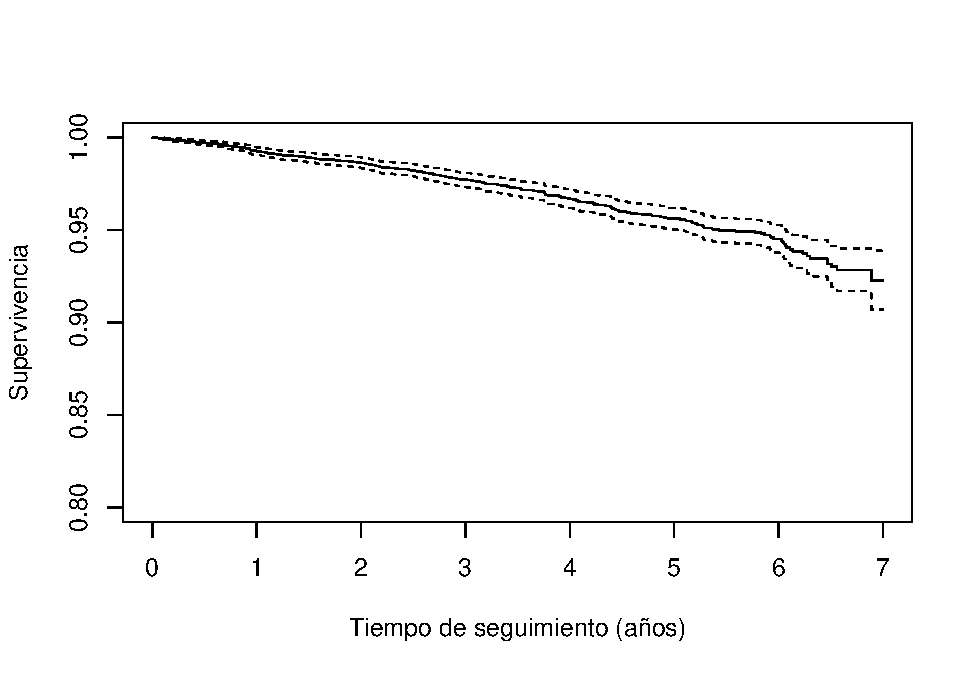
\includegraphics{fig_out/unnamed-chunk-153-1.pdf}

Si quisiéramos calcular Kaplan-Meier para distrintos grupos, por ejemplo para el los distintos grupos de intervención de nuestro estudio, bastaría con escribir:

\begin{Shaded}
\begin{Highlighting}[]
\NormalTok{ans.km.group }\OtherTok{\textless{}{-}} \FunctionTok{survfit}\NormalTok{(}\FunctionTok{Surv}\NormalTok{(toevent, event}\SpecialCharTok{==}\StringTok{\textquotesingle{}Yes\textquotesingle{}}\NormalTok{) }\SpecialCharTok{\textasciitilde{}}\NormalTok{ group, predimed)}
\FunctionTok{plot}\NormalTok{(ans.km.group, }\AttributeTok{ylim=}\FunctionTok{c}\NormalTok{(}\FloatTok{0.8}\NormalTok{,}\DecValTok{1}\NormalTok{), }
     \AttributeTok{xlab=}\StringTok{"Tiempo de seguimiento (años)"}\NormalTok{, }
     \AttributeTok{ylab=}\StringTok{"Supervivencia"}\NormalTok{, }\AttributeTok{col=}\DecValTok{1}\SpecialCharTok{:}\DecValTok{3}\NormalTok{)}
\FunctionTok{legend}\NormalTok{(}\StringTok{"bottomleft"}\NormalTok{, }\FunctionTok{levels}\NormalTok{(predimed}\SpecialCharTok{$}\NormalTok{group), }
       \AttributeTok{lty=}\DecValTok{1}\NormalTok{, }\AttributeTok{col=}\DecValTok{1}\SpecialCharTok{:}\DecValTok{3}\NormalTok{, }\AttributeTok{bty=}\StringTok{"n"}\NormalTok{)}
\end{Highlighting}
\end{Shaded}

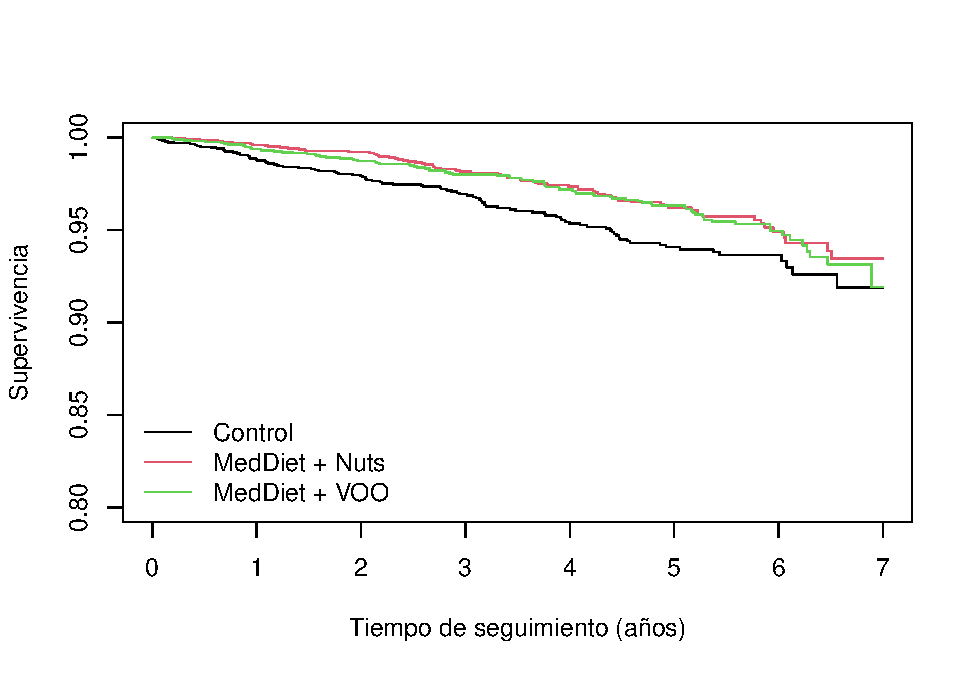
\includegraphics{fig_out/unnamed-chunk-154-1.pdf}

Finalmente, podemos comparar las curvas de supervivencia entre grupos con la función \texttt{survdiff} que tiene implementado por defecto, el test de log-rank:

\begin{Shaded}
\begin{Highlighting}[]
\FunctionTok{survdiff}\NormalTok{(}\FunctionTok{Surv}\NormalTok{(toevent, event}\SpecialCharTok{==}\StringTok{\textquotesingle{}Yes\textquotesingle{}}\NormalTok{) }\SpecialCharTok{\textasciitilde{}}\NormalTok{ group, predimed)}
\end{Highlighting}
\end{Shaded}

\begin{verbatim}
Call:
survdiff(formula = Surv(toevent, event == "Yes") ~ group, data = predimed)

                        N Observed Expected
group=Control        2042       97     75.4
group=MedDiet + Nuts 2100       70     82.7
group=MedDiet + VOO  2182       85     93.9
                     (O-E)^2/E (O-E)^2/V
group=Control            6.194      8.85
group=MedDiet + Nuts     1.946      2.90
group=MedDiet + VOO      0.848      1.35

 Chisq= 9  on 2 degrees of freedom, p= 0.01 
\end{verbatim}

Podemos concluir que las diferencias observadas en las curvas de supervivencia, son significativamente distintas ya que el p-valor del test de log-rank es \$\textless0.5\%.

Este test considera que todas las diferencias observadas a lo largo del tiempo son igual de imporatantes. A veces, queremos dar más peso a las diferencias observadas al inicio del estudio. En ese caso, el test más potente es el del Wilcoxon que puede calcularse de la misma manera, pero usando el argumento \texttt{rho=1}

\begin{Shaded}
\begin{Highlighting}[]
\FunctionTok{survdiff}\NormalTok{(}\FunctionTok{Surv}\NormalTok{(toevent, event}\SpecialCharTok{==}\StringTok{\textquotesingle{}Yes\textquotesingle{}}\NormalTok{) }\SpecialCharTok{\textasciitilde{}}\NormalTok{ group, predimed, }\AttributeTok{rho =} \DecValTok{1}\NormalTok{)}
\end{Highlighting}
\end{Shaded}

\begin{verbatim}
Call:
survdiff(formula = Surv(toevent, event == "Yes") ~ group, data = predimed, 
    rho = 1)

                        N Observed Expected
group=Control        2042     95.0     73.6
group=MedDiet + Nuts 2100     68.1     80.7
group=MedDiet + VOO  2182     82.7     91.6
                     (O-E)^2/E (O-E)^2/V
group=Control            6.222      9.11
group=MedDiet + Nuts     1.952      2.98
group=MedDiet + VOO      0.857      1.40

 Chisq= 9.3  on 2 degrees of freedom, p= 0.01 
\end{verbatim}

Llegamos a la misma conclusión que con el test de log-rank, pero notemos que el valor del estadistico (Chisq) es ligeramente superior, por lo que el p-valor es menor (es decir, más significativo) y nos daría más evidencias en contra de la hipótesis nula (notemos que aquí vemos 0.01 en ambos casos por un tema de redondeo).

Podemos mejorar la visualización usando la función \texttt{ggsurvplot\ ()} de la librería \texttt{survminer}. Una caída vertical en las curvas indica un evento. Una marca vertical en las curvas significa que un individuo fue censurado.

\begin{Shaded}
\begin{Highlighting}[]
\FunctionTok{library}\NormalTok{(survminer)}
\FunctionTok{ggsurvplot}\NormalTok{(}
\NormalTok{  ans.km, }\AttributeTok{ylim=}\FunctionTok{c}\NormalTok{(}\FloatTok{0.9}\NormalTok{,}\DecValTok{1}\NormalTok{),}
  \AttributeTok{pval =} \ConstantTok{TRUE}\NormalTok{,}
  \AttributeTok{conf.int =} \ConstantTok{TRUE}\NormalTok{,}
  \AttributeTok{risk.table =} \ConstantTok{TRUE}\NormalTok{,}
  \AttributeTok{ggtheme =} \FunctionTok{theme\_bw}\NormalTok{(),}
  \AttributeTok{title =} \StringTok{"Estimación de la supervivencia con Kaplan{-}Meier"}
\NormalTok{)}
\end{Highlighting}
\end{Shaded}

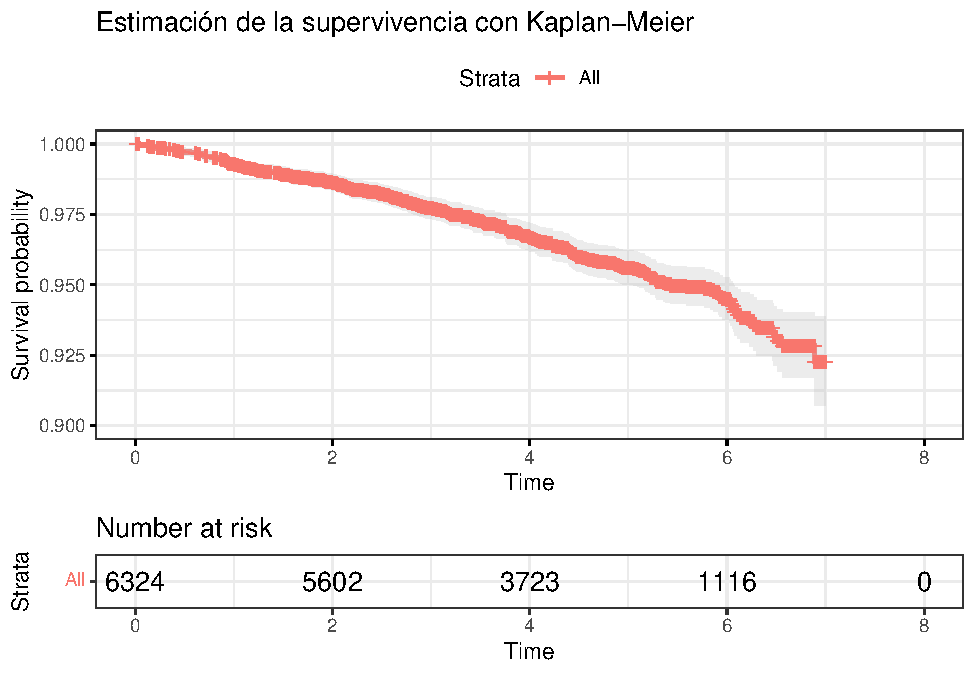
\includegraphics{fig_out/plotkm2-1.pdf}

NOTA: la opción \texttt{pval=TRUE} nos permitiría ver el p-valor de Kaplan-Meier en el gráfico, pero puesto que hemos indicado que el eje Y se vea sólo de 0.9 a 1, el p-valor no se ve. Si se vería en caso de quitar la opción de \texttt{ylim} aunque entonces las curvas se verían muy juntas. Existen opciones para poder ``tunear'' esta visualización usando la función \texttt{annotate()}.

\hypertarget{funciones-involucradas-en-el-anuxe1lisis-de-supervivencia}{%
\section{Funciones involucradas en el análisis de supervivencia}\label{funciones-involucradas-en-el-anuxe1lisis-de-supervivencia}}

Aparte de la función de supervivencia que se define como:

\begin{itemize}
\tightlist
\item
  \textbf{Supervivencia:} probabilidad de estar libre de evento en el momento \(t\) (se supone que el evento ocurre después)
\end{itemize}

\[S(t) = \text{Pr}(T>t)\]

Existen otras medidas para resumir este tipo de estudios que pueden ser interesantes según el contexto. Por ejemplo, si nos interesa cuantificar la probabilidad de observar nuestro evento de interés (normalemete cuanod el evento no es ``malo'' como en el análisis de supervivencia tradicional que el evento es la muerte) podemos calcular la función de:

\begin{itemize}
\tightlist
\item
  \textbf{Distribución}: probabilidad de evento antes de tiempo \(t\). Es el complementario de la función de supervivencia
\end{itemize}

\[\text{Pr}(T\leq t) = 1-S(t)\]

Otras medidas interesantes son:

\begin{itemize}
\tightlist
\item
  \textbf{Hazard} (riesgo instantaneo): Es la probabilidad que ocurra el evento en un intervalo infinitamente pequeño dado que no lo ha tenido hasta el momento \(t\)
\end{itemize}

\[\lambda(t) = \lim_{\delta \rightarrow 0} \frac{\text{Pr}\left(T \in (t, t+\delta) \right)}{S(t)} \]

\begin{itemize}
\tightlist
\item
  \textbf{Cumulative Hazard} (riesgo acumulado): es la suma o integral del riesgo instantáneo hasta el momento \(t\)
\end{itemize}

\[\Lambda(t) = \int_{0}^{t} \lambda(s) ds\]
Existe la siguiente relación entre el riesgo acumulado y la función de supervivencia

\[S(t) = \text{exp} \left(-\Lambda(t)\right)\]
o bien

\[\Lambda(t) = -\text{ln}\left(S(t)\right)\]

Todas estas funciones se pueden calcular conla función \texttt{ggsurvplot()} cambiando el argumento \texttt{fun}. Por ejemplo la función de probabilidad se calcularía mediante la opción ``event'' y la de riesgo acumulado con ``cumhaz''

\begin{Shaded}
\begin{Highlighting}[]
\FunctionTok{ggsurvplot}\NormalTok{(}
\NormalTok{  ans.km, }\AttributeTok{ylim=}\FunctionTok{c}\NormalTok{(}\DecValTok{0}\NormalTok{,.}\DecValTok{1}\NormalTok{),}
  \AttributeTok{fun =} \StringTok{"event"}\NormalTok{,}
  \AttributeTok{conf.int =} \ConstantTok{TRUE}\NormalTok{,}
  \AttributeTok{risk.table =} \ConstantTok{TRUE}\NormalTok{,}
  \AttributeTok{ggtheme =} \FunctionTok{theme\_bw}\NormalTok{(),}
  \AttributeTok{title =} \StringTok{"Estimación de la función de distribución con Kaplan{-}Meier"}
\NormalTok{)}
\end{Highlighting}
\end{Shaded}

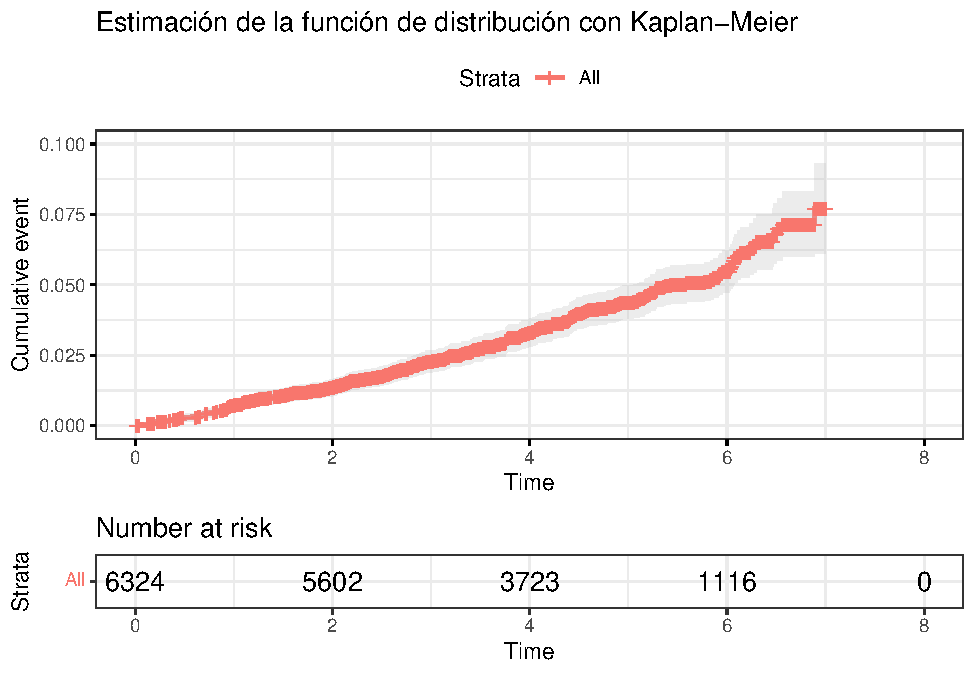
\includegraphics{fig_out/unnamed-chunk-157-1.pdf}

\hypertarget{modelo-de-regresiuxf3n-de-cox}{%
\section{Modelo de regresión de Cox}\label{modelo-de-regresiuxf3n-de-cox}}

Normalmente queremos estudiar cómo influye más de una variable en la supervivencia. Para este caso, necesitamos utilizar modelos de regresión. Los modelos de regresión de Cox sirven para evaluar el efecto de distintas variables sobre el tiempo hasta el evento, o para crear un moelo de predicción.

Los modelos de cox asumen \textbf{riesgos proporcionales}, esto es, se separa el riesgo (``Hazard'') de paceder un evento antes del momento \(t\) como un producto del

\begin{itemize}
\item
  \(\Lambda_0(t)\): riesgo basal, cuando todas las variables independientes \(x\) valen cero) y
\item
  \(\sum_{k=1} \beta_k x_{ik}\): combinación lineal de las variables independientes (predictor lineal).
\end{itemize}

\[\Lambda(t|\vec{x}_i) = \Lambda_0(t)\cdot \text{exp}\left(\sum_{k=1} \beta_k x_{ik}\right)\]

donde los coeficientes \(\beta_k\) son los log-Hazard Ratios.

Cox propone un método para estimar los coeficientes \(\beta_k\) sin suponer ninguna distribución sobre la variable respuesta \(T\) (tiempo hasta evento). Por esto se llama método semiparamétrico y se basa en estimar la ``partial-likelihood''.

Existen otros métodos que suponen una distribución de la \(T\), y por lo tanto parametrizan la incidencia basal \(\Lambda_0(t)\). Por ejemplo,la regresión de Weibull que supone una distribución Weibull sobre \(T\). Una de las ventaja que tienen los métodos no paramétricos es que permiten estimar la media o la mediana de \(T\) aunque más de la mitad de los individuos de la muestra estén censurados (o sea, que no se llegue al 50\% de eventos en el seguimiento). La desventaja es que suponen una distribución sobre \(T\) que puede no ser correcta y que conllevaría a resultados sesgados. En biomedicina, el método más usado es el de los modelos de Cox y es el que estudiaremos en este curso.

\textbf{Ejemplo}

Para ajustar un modelo de Cox en R se usa la función \texttt{coxph} de la librería \texttt{survival}.

\begin{Shaded}
\begin{Highlighting}[]
\NormalTok{modelo }\OtherTok{\textless{}{-}} \FunctionTok{coxph}\NormalTok{(}\FunctionTok{Surv}\NormalTok{(toevent, event}\SpecialCharTok{==}\StringTok{\textquotesingle{}Yes\textquotesingle{}}\NormalTok{)}\SpecialCharTok{\textasciitilde{}}\NormalTok{age}\SpecialCharTok{+}\NormalTok{sex}\SpecialCharTok{+}\NormalTok{p14}\SpecialCharTok{+}\NormalTok{group, predimed)}
\end{Highlighting}
\end{Shaded}

Hay diferentes aspectos a validar del modelo de Cox. Entre ellos la proporcionalidad de los efectos. Quiere decir que se supone que las \(\beta_k\) no dependen del tiempo (por ejemplo, el efecto del sexo es el mismo tanto a 1 años como a 5 años). Ésto se puede comprovar mediante la siguiente función:

\begin{Shaded}
\begin{Highlighting}[]
\FunctionTok{cox.zph}\NormalTok{(modelo)}
\end{Highlighting}
\end{Shaded}

\begin{verbatim}
         chisq df     p
age    0.33102  1 0.565
sex    0.17845  1 0.673
p14    0.00189  1 0.965
group  5.75156  2 0.056
GLOBAL 6.35652  5 0.273
\end{verbatim}

Aparece un p-valor para cada variable y uno global. En este caso parece que se cumple la proporcionalidad para todas las variables ya que el p-valor no es \(<0.05\) y por lo tanto no podemos rechazar la hipótesis nula que es que los riesgos son proporcionales. No obstante, si no se cumpliera la proporcionalidad de una variable categórica, por ejemplo el sexo, ésta se puede poner como \texttt{strata} (se asume una curva de indidencia basal \(\Lambda_0(t)\) para cada sexo) y se solucionaría el problema. Cuando esto no ocurre para una variable continua, debemos hacer modelos más avanzados que contemplan la posibilidad de introducir en el modelo una variable dependiente del tiempo (que veremos más adelante).

\begin{Shaded}
\begin{Highlighting}[]
\NormalTok{modelo2 }\OtherTok{\textless{}{-}} \FunctionTok{coxph}\NormalTok{(}\FunctionTok{Surv}\NormalTok{(toevent, event}\SpecialCharTok{==}\StringTok{\textquotesingle{}Yes\textquotesingle{}}\NormalTok{)}\SpecialCharTok{\textasciitilde{}}\NormalTok{age}\SpecialCharTok{+}\FunctionTok{strata}\NormalTok{(sex)}\SpecialCharTok{+}\NormalTok{p14}\SpecialCharTok{+}\NormalTok{group, predimed)}
\FunctionTok{summary}\NormalTok{(modelo2)}
\end{Highlighting}
\end{Shaded}

\begin{verbatim}
Call:
coxph(formula = Surv(toevent, event == "Yes") ~ age + strata(sex) + 
    p14 + group, data = predimed)

  n= 6324, number of events= 252 

                        coef exp(coef) se(coef)
age                  0.06790   1.07026  0.01010
p14                 -0.12221   0.88497  0.03046
groupMedDiet + Nuts -0.39498   0.67369  0.15771
groupMedDiet + VOO  -0.31459   0.73009  0.14894
                         z Pr(>|z|)    
age                  6.720 1.82e-11 ***
p14                 -4.012 6.03e-05 ***
groupMedDiet + Nuts -2.505   0.0123 *  
groupMedDiet + VOO  -2.112   0.0347 *  
---
Signif. codes:  
0 '***' 0.001 '**' 0.01 '*' 0.05 '.' 0.1 ' ' 1

                    exp(coef) exp(-coef)
age                    1.0703     0.9344
p14                    0.8850     1.1300
groupMedDiet + Nuts    0.6737     1.4844
groupMedDiet + VOO     0.7301     1.3697
                    lower .95 upper .95
age                    1.0493    1.0917
p14                    0.8337    0.9394
groupMedDiet + Nuts    0.4946    0.9177
groupMedDiet + VOO     0.5453    0.9776

Concordance= 0.652  (se = 0.018 )
Likelihood ratio test= 71.75  on 4 df,   p=1e-14
Wald test            = 72.99  on 4 df,   p=5e-15
Score (logrank) test = 73.94  on 4 df,   p=3e-15
\end{verbatim}

En este gráfico se obtiene una curva de supervivencia para cada sexo, ajustado por las demás covariables (nota que en esta gráfica se asume que el efecto de las demás covariables es el mismo para ambos sexos).

\begin{Shaded}
\begin{Highlighting}[]
\FunctionTok{plot}\NormalTok{(}\FunctionTok{survfit}\NormalTok{(modelo2), }\AttributeTok{ylim=}\FunctionTok{c}\NormalTok{(}\FloatTok{0.8}\NormalTok{,}\DecValTok{1}\NormalTok{), }\AttributeTok{lty=}\DecValTok{1}\SpecialCharTok{:}\DecValTok{2}\NormalTok{)}
\FunctionTok{legend}\NormalTok{(}\StringTok{"bottomleft"}\NormalTok{, }\FunctionTok{levels}\NormalTok{(predimed}\SpecialCharTok{$}\NormalTok{sex), }\AttributeTok{lty=}\DecValTok{1}\SpecialCharTok{:}\DecValTok{2}\NormalTok{, }\AttributeTok{bty=}\StringTok{"n"}\NormalTok{)}
\end{Highlighting}
\end{Shaded}

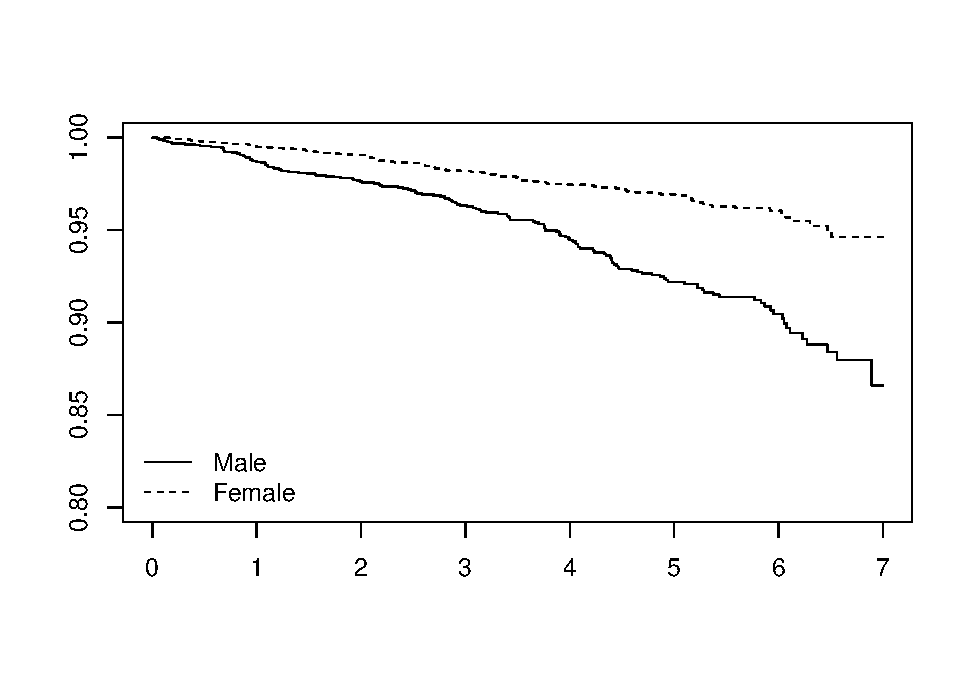
\includegraphics{fig_out/unnamed-chunk-161-1.pdf}

\hypertarget{efectos-tiempo-dependientes}{%
\subsection{Efectos tiempo-dependientes}\label{efectos-tiempo-dependientes}}

El efecto tiempo-dependiente (no confundir con variables tiempo-dependientes) se da cuando el efecto de una variable \(\beta_k\) no es constante a lo largo del tiempo. En este caso, como se ha comentado anteriormente, si se trata de una variable categórica se puede poner en el modelo como \texttt{strata}. Si se trata de una variable continua, se puede incorporar la interacción de la variable \(x_k\) con el tiempo.
Otra estrategia que se usa habitualmente es dividir el tiempo de seguimiento en dos o tres tramos (a corto y a largo plazo), y realizar análisis por separado.

De la anterior ecuación sobre la incidencia acumulada, se suponía que los efectos eran fijos y no dependían del tiempo. Pero si dependieran del tiempo en general se debería reescribir como:

\[\Lambda(t|\vec{x}_i) = \Lambda_0(t)\cdot \text{exp}\left(\sum_{k=1} \color{blue}{\beta_k(t)} x_{ik}\right)\]
donde \(\beta_k(t)\) representa una función del tiempo.

Este tipo de modelos con efectos tiempo dependientes no los veremos en este curso, sin embargo nos centraremos en otro aspecto fundamental que se da en estudios longitudinales que es el hecho de recoger una variable explicativa en distintos momentos del tiempo (variales tiempo-dependientes).

\hypertarget{variables-tiempo-dependientes-datos-longitudinales}{%
\subsection{Variables tiempo-dependientes (datos longitudinales)}\label{variables-tiempo-dependientes-datos-longitudinales}}

Los modelos con variables tiempo-dependientes se tienen cuando en el seguimiento de los individuos de la muestra también se han ido actualizando los valores de todas o algunas de las variables indepndientes (\(x_k\)). Por ejemplo, el nivel de colesterol se puede recoger al inicio del estudio e introducir esa variable en el modelo de Cox para ver si influencia en el tiempo hasta sufrir un infarto de miocardio, pero también podemos recoger el nivel de colesterol en distintos momentos temporales y ver si esta variable cambiante a lo largo del tiempo se asocia con nuestro evento de interés.

Así pues, en cada momento \(t\) el riesgo acumulado se tiene que estimar teniendo en cuenta el valor que toma cada \(x_k\) en dicho tiempo \(t\). Esto se puede formular de la siguiente manera

\[\Lambda(t|\vec{x}_i = \Lambda_0(t)\cdot \text{exp}\left(\sum_{k=1} \beta_k \color{blue}{x_{itk}}\right)\]
donde \(x_{itk}\) representa el valor de la variable \(x_k\) del individuo \(i\) en el momento \(t\)

\hypertarget{estructura-de-los-datos-1}{%
\subsection{Estructura de los datos}\label{estructura-de-los-datos-1}}

Para ajustar estos modelos, el reto principal (y único), es estructurar bien la base de datos. Así, para cada individuo tendremos tantas filas como actualizaciones tengamos de cada variable \(x_k\). Además hay que anotar el momento de estos cambios. Adicionalemente tendremos una fila final donde se indicará el tiempo de evento o censura para nuestro evento de interés.

Veámoslo con un ejemplo: Utilizaremos la base de datos \texttt{aids} de la librería \texttt{JM}

\begin{Shaded}
\begin{Highlighting}[]
\FunctionTok{library}\NormalTok{(JM)}
\FunctionTok{data}\NormalTok{(aids)}
\FunctionTok{head}\NormalTok{(aids)}
\end{Highlighting}
\end{Shaded}

\begin{verbatim}
  patient  Time death       CD4 obstime drug
1       1 16.97     0 10.677078       0  ddC
2       1 16.97     0  8.426150       6  ddC
3       1 16.97     0  9.433981      12  ddC
4       2 19.00     0  6.324555       0  ddI
5       2 19.00     0  8.124038       6  ddI
6       2 19.00     0  4.582576      12  ddI
  gender prevOI         AZT start  stop event
1   male   AIDS intolerance     0  6.00     0
2   male   AIDS intolerance     6 12.00     0
3   male   AIDS intolerance    12 16.97     0
4   male noAIDS intolerance     0  6.00     0
5   male noAIDS intolerance     6 12.00     0
6   male noAIDS intolerance    12 18.00     0
\end{verbatim}

En esta base de datos tenemos diferentes participantes en los que se ha tomado distintas medidas de la variable CD4. La variable \texttt{obstime} indica cuándo se han tomado las medidas de CD4. Mientras que la variable \texttt{time} y \texttt{death} indica el tiempo observado y si el individuo se ha muerto (1) o sigue vivo (0, dato censurado) al finalizar el seguimiento. En este caso el evento de interés es la muerte y los individuos vivos serán los censurados. La variable tiempo-dependiente es la variable CD4. Nuestro objetivo final es demostrar si hay diferencias en la mortalidad entre dos fármacos (variable `drug': ddI = didanosine; ddC = zalcitabine.) ajustando por la variable `gender'.

Para ajustar un modelo con variables tiempo-dependientes se ha de reestructurar esta base de datos. Para ello debemos llevar a cabo los siguientes pasos

\begin{enumerate}
\def\labelenumi{\arabic{enumi}.}
\tightlist
\item
  Creamos una base de datos con una fila por individuo, con los tiempos de muerte y las covariables de interés (fijas, no cambiantes a lo largo del tiempo - en nuestro caso `drug' , `gender') y creamos la variable \texttt{endpt}.
\end{enumerate}

\begin{Shaded}
\begin{Highlighting}[]
\NormalTok{temp }\OtherTok{\textless{}{-}}\NormalTok{ aids }\SpecialCharTok{\%\textgreater{}\%}\NormalTok{ dplyr}\SpecialCharTok{::}\FunctionTok{select}\NormalTok{(patient, Time, death, drug, gender)}
\NormalTok{x }\OtherTok{\textless{}{-}} \FunctionTok{rep}\NormalTok{(}\DecValTok{1}\NormalTok{,}\FunctionTok{nrow}\NormalTok{(temp))}
\NormalTok{datos }\OtherTok{\textless{}{-}} \FunctionTok{aggregate}\NormalTok{(x, temp, sum)}
\NormalTok{datos }\OtherTok{\textless{}{-}} \FunctionTok{tmerge}\NormalTok{(datos, datos, }\AttributeTok{id=}\NormalTok{patient, }\AttributeTok{endpt =} \FunctionTok{event}\NormalTok{(Time, death))}
\FunctionTok{head}\NormalTok{(datos)}
\end{Highlighting}
\end{Shaded}

\begin{verbatim}
  patient  Time death drug gender x tstart tstop
1     351 12.27     0  ddC female 4      0 12.27
2     305 12.30     0  ddC female 2      0 12.30
3     336 12.57     0  ddC female 3      0 12.57
4     268 12.73     0  ddC female 4      0 12.73
5     160 13.20     0  ddC female 3      0 13.20
6     377 13.50     0  ddC female 4      0 13.50
  endpt
1     0
2     0
3     0
4     0
5     0
6     0
\end{verbatim}

\begin{enumerate}
\def\labelenumi{\arabic{enumi}.}
\setcounter{enumi}{1}
\tightlist
\item
  Luego, hacemos uso de la función \texttt{tmerge()} para crear la base de datos en el formato deseado. Las variables tiempo dependientes se especifican mediante la función \texttt{tdc} en que se indica también la variable que recoge cuando se han tomado sus medidas (en nuestro caso `obstime').
\end{enumerate}

\begin{Shaded}
\begin{Highlighting}[]
\NormalTok{aids2 }\OtherTok{\textless{}{-}} \FunctionTok{tmerge}\NormalTok{(datos, aids, }\AttributeTok{id=}\NormalTok{patient, }\AttributeTok{CD4 =} \FunctionTok{tdc}\NormalTok{(obstime, CD4))}
\FunctionTok{head}\NormalTok{(aids2)}
\end{Highlighting}
\end{Shaded}

\begin{verbatim}
  patient  Time death drug gender x tstart tstop
1     351 12.27     0  ddC female 4      0  2.00
2     351 12.27     0  ddC female 4      2  6.00
3     351 12.27     0  ddC female 4      6 12.00
4     351 12.27     0  ddC female 4     12 12.27
5     305 12.30     0  ddC female 2      0  6.00
6     305 12.30     0  ddC female 2      6 12.30
  endpt      CD4
1     0 5.477226
2     0 6.403124
3     0 4.690416
4     0 4.000000
5     0 2.000000
6     0 2.449490
\end{verbatim}

\hypertarget{ajuste-del-modelo}{%
\subsection{Ajuste del modelo}\label{ajuste-del-modelo}}

En esta nueva base de datos, tenemos intervalos de tiempo \texttt{tstart} y \texttt{tstop} que se usará como tiempos de supervivencia en la función \texttt{Surv} y que ayuda a dividir el seguimento en los intervalos donde CD4 has sido observado de forma diferente para cada invididuo. Con esta información, podremos usar la función \texttt{coxph\ ()} de la forma habitual, pero usando esta nueva escala de tiempo:

\begin{Shaded}
\begin{Highlighting}[]
\NormalTok{modelo }\OtherTok{\textless{}{-}} \FunctionTok{coxph}\NormalTok{(}\FunctionTok{Surv}\NormalTok{(tstart, tstop, endpt) }\SpecialCharTok{\textasciitilde{}}\NormalTok{ CD4 }\SpecialCharTok{+}\NormalTok{ drug }\SpecialCharTok{+}\NormalTok{ gender, }\AttributeTok{data=}\NormalTok{aids2)}
\FunctionTok{summary}\NormalTok{(modelo)}
\end{Highlighting}
\end{Shaded}

\begin{verbatim}
Call:
coxph(formula = Surv(tstart, tstop, endpt) ~ CD4 + drug + gender, 
    data = aids2)

  n= 1405, number of events= 188 

               coef exp(coef) se(coef)      z
CD4        -0.19440   0.82333  0.02434 -7.986
drugddI     0.31698   1.37298  0.14669  2.161
gendermale -0.32579   0.72196  0.24248 -1.344
           Pr(>|z|)    
CD4         1.4e-15 ***
drugddI      0.0307 *  
gendermale   0.1791    
---
Signif. codes:  
0 '***' 0.001 '**' 0.01 '*' 0.05 '.' 0.1 ' ' 1

           exp(coef) exp(-coef) lower .95
CD4           0.8233     1.2146    0.7850
drugddI       1.3730     0.7283    1.0299
gendermale    0.7220     1.3851    0.4489
           upper .95
CD4           0.8636
drugddI       1.8303
gendermale    1.1612

Concordance= 0.697  (se = 0.018 )
Likelihood ratio test= 96.28  on 3 df,   p=<2e-16
Wald test            = 67.58  on 3 df,   p=1e-14
Score (logrank) test = 75.22  on 3 df,   p=3e-16
\end{verbatim}

Notemos que que tanto las variables tiempo-dependientes (en este caso CD4) como las no-tiempo-dependientes (\texttt{drug} y \texttt{gender}) se ponen de la misma manera y de forma habitual en la fórmula.

La interpretación de los resultados es exactamente la misma que para un modelo de Cox sin variables tiempo-dependientes.

\textbf{Comparación con el modelo sin variables tiempo-dependientes}

Estos resultados los podríamos comparar con el caso en el que consideráramos la primera medida de CD4 como una variable fija a lo largo del tiempo:

\begin{Shaded}
\begin{Highlighting}[]
\NormalTok{aids1obs }\OtherTok{\textless{}{-}} \FunctionTok{subset}\NormalTok{(aids, obstime}\SpecialCharTok{==}\DecValTok{0}\NormalTok{)}
\NormalTok{modelo1obs }\OtherTok{\textless{}{-}} \FunctionTok{coxph}\NormalTok{(}\FunctionTok{Surv}\NormalTok{(Time, death) }\SpecialCharTok{\textasciitilde{}}\NormalTok{ CD4 }\SpecialCharTok{+}\NormalTok{ drug }\SpecialCharTok{+}\NormalTok{ gender, aids1obs)}
\FunctionTok{summary}\NormalTok{(modelo1obs)}
\end{Highlighting}
\end{Shaded}

\begin{verbatim}
Call:
coxph(formula = Surv(Time, death) ~ CD4 + drug + gender, data = aids1obs)

  n= 467, number of events= 188 

               coef exp(coef) se(coef)      z
CD4        -0.18295   0.83281  0.02222 -8.232
drugddI     0.26694   1.30597  0.14648  1.822
gendermale -0.20238   0.81679  0.24216 -0.836
           Pr(>|z|)    
CD4          <2e-16 ***
drugddI      0.0684 .  
gendermale   0.4033    
---
Signif. codes:  
0 '***' 0.001 '**' 0.01 '*' 0.05 '.' 0.1 ' ' 1

           exp(coef) exp(-coef) lower .95
CD4           0.8328     1.2008    0.7973
drugddI       1.3060     0.7657    0.9801
gendermale    0.8168     1.2243    0.5081
           upper .95
CD4           0.8699
drugddI       1.7403
gendermale    1.3129

Concordance= 0.703  (se = 0.019 )
Likelihood ratio test= 92.54  on 3 df,   p=<2e-16
Wald test            = 70.82  on 3 df,   p=3e-15
Score (logrank) test = 78.19  on 3 df,   p=<2e-16
\end{verbatim}

Notemos que utilizando este modelo, nuestra conclusión sería que no hay diferencias en la supervivencia entre fármacos (`drug') mientras que el modelo utilizando datos longitudinales para CD4 muestra que la didanosine (ddI) tiene una peor supervivencia (p = 0.0307).

Una vez más se demuestra que, en estadística, uno puede usar cualquier modelo para analizar sus datos y obtener resultados similares (en este segundo modelo casi sale significativo). Sin embargo, si no se utiliza el modelo correcto el perjudicado es el investigador, ya que, la utilización del modelo correcto proporciona el test más potente para detectar diferencias cuando realmente las hay. Es como el caso de analizar una variable 0,1 para comparar dos grupos y usar la t de Student. R nos dará un p-valor, pero este no será el test más potente para encontrar diferencias cuando realmente las haya, ya que ese test es el más potente cuando los datos son normales. Es por ello que en estos casos se usa la chi-cuadrado.

\textbf{Validación del modelo}

La validación del modelo con variables tiempo-dependientes se hace de la misma manera que para el modelo de Cox ``clásico''. Por ejemplo, también se puede aplicar la función \texttt{coxz.ph}. Sin embargo, la discriminación y la calibración que necesitan del cálculo del riesgo predicho a tiempo \(t_0\) no és fácil de calcular: ¿cómo se tiene en cuenta que el valor de \(x_k\) cambia y que ello conlleva a un cambio del riesgo acumulado \(\Lambda\)?.

\begin{Shaded}
\begin{Highlighting}[]
\FunctionTok{cox.zph}\NormalTok{(modelo)}
\end{Highlighting}
\end{Shaded}

\begin{verbatim}
        chisq df    p
CD4    0.2875  1 0.59
drug   0.0034  1 0.95
gender 1.6437  1 0.20
GLOBAL 1.9692  3 0.58
\end{verbatim}

\textbf{Términos no lineales: ``splines''}

También, como en los modelo de Cox ``clásicos'' se pueden introducir términos polinómicos o de splines (\texttt{psplines}) para modelar efectos no lineases de las variables \(x_k\) cuantitativas.

\begin{Shaded}
\begin{Highlighting}[]
\NormalTok{modelo.splines }\OtherTok{\textless{}{-}} \FunctionTok{coxph}\NormalTok{(}\FunctionTok{Surv}\NormalTok{(tstart, tstop, endpt) }\SpecialCharTok{\textasciitilde{}} \FunctionTok{pspline}\NormalTok{(CD4) }\SpecialCharTok{+}\NormalTok{ drug }\SpecialCharTok{+}\NormalTok{ gender, }\AttributeTok{data=}\NormalTok{aids2)}
\FunctionTok{coef}\NormalTok{(}\FunctionTok{summary}\NormalTok{(modelo.splines))}
\end{Highlighting}
\end{Shaded}

\begin{verbatim}
                           coef   se(coef)
pspline(CD4), linear -0.1900175 0.02553879
pspline(CD4), nonlin         NA         NA
drugddI               0.3164310 0.14684398
gendermale           -0.3282002 0.24253118
                            se2     Chisq
pspline(CD4), linear 0.02527049 55.358799
pspline(CD4), nonlin         NA  5.669855
drugddI              0.14682270  4.643503
gendermale           0.24249275  1.831229
                           DF            p
pspline(CD4), linear 1.000000 1.004194e-13
pspline(CD4), nonlin 3.092747 1.367478e-01
drugddI              1.000000 3.117131e-02
gendermale           1.000000 1.759825e-01
\end{verbatim}

\begin{Shaded}
\begin{Highlighting}[]
\FunctionTok{termplot}\NormalTok{(modelo, }\AttributeTok{terms=}\DecValTok{1}\NormalTok{, }\AttributeTok{se=}\ConstantTok{TRUE}\NormalTok{, }\AttributeTok{rug=}\ConstantTok{TRUE}\NormalTok{)}
\end{Highlighting}
\end{Shaded}

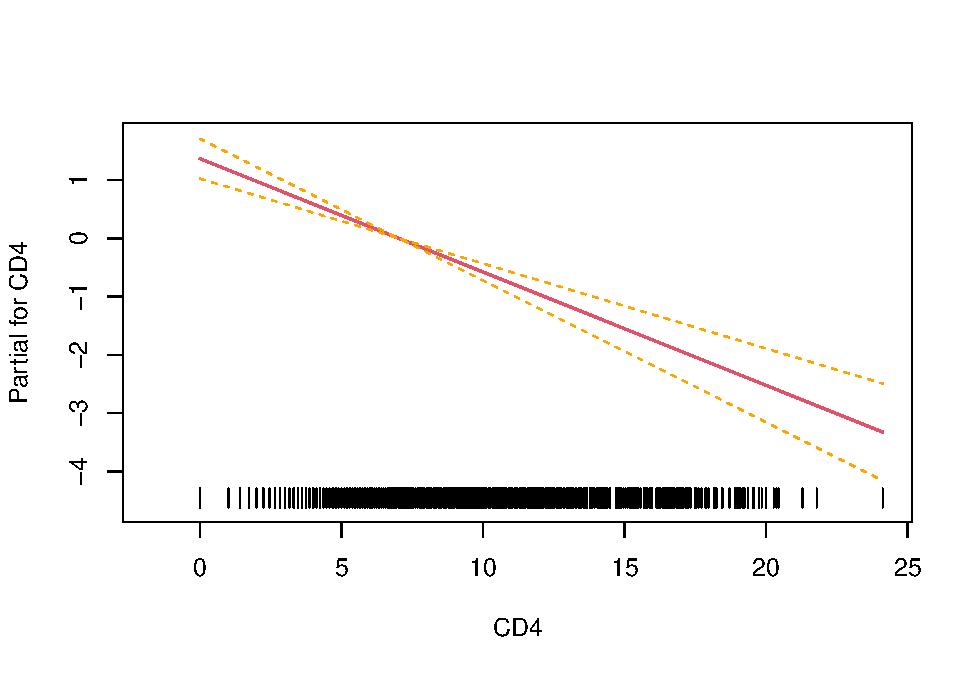
\includegraphics{fig_out/unnamed-chunk-168-1.pdf}

en nuestro ejemplo, se demuestra que el efecto de CD4 es lineal (no hay términos cuadráticos, ni cúbicos, ni puntos de inflexión o cambios de tendencias, \ldots) por lo que el modelo sin splines ya sería suficiente para modelar nuestros datos.

\hypertarget{joint-models-para-datos-longitudinales-y-datos-de-supervivencia}{%
\chapter{Joint models para datos longitudinales y datos de supervivencia}\label{joint-models-para-datos-longitudinales-y-datos-de-supervivencia}}

En el capítulo anterior hemos visto cómo modelar una variable dependiente que mide el tiempo hasta una variable de interés (análisis de supervivencia). Vimos también cómo tener en cuenta como estimar modelos de supervivencia cuando una variable independiente es medida a lo largo del tiempo. En este tema, iremos un paso más allá y nos interesaremos por unos modelos en los que nuestra variable resultado está formada por dos tipos de variables: una variable respuesta medida de forma longitudinal y otra que recoge el tiempo hasta un evento de interés. A estos modelo se les comonce como \textbf{``Joint Models''}. Estos modelos tienen en cuenta las variables tiempo-dependientes para modelizar el tiempo hasta evento con posible censura por la derecha. Estos modelos surgen cuando hay valores faltantes en algunas medidas de las variables \(x_k\). Para solventarlo, modelizan una regresión de supervivencia de Cox, y en lugar de condicionar por los valores observados de \(x_k\), se condiciona por los valores ajustados de ellos según modelos de datos longitudinales que pueden ser los modelos mixtos. De esta forma se \textbf{fusiona los modelos de medidas repetidas con los modelos de Cox.}.

En este curso mostraremos cómo llevar a cabo estos análisis mediante la librería \texttt{JM}, pero debemos tener en cuenta que también podemos usar la librería \textbf{\texttt{joineR}} para ajustar este tipo de modelos. Esta librería también tiene incorporadas funciones y opciones para tener encuenta \textbf{eventos competitivos}, es decir, cuando nuestro evento de interés no es uno sólo si no más de uno.

\hypertarget{por-quuxe9-deberuxedamos-utilizar-este-tipo-de-modelos}{%
\section{¿Por qué deberíamos utilizar este tipo de modelos?}\label{por-quuxe9-deberuxedamos-utilizar-este-tipo-de-modelos}}

Como mencionamos en la sección anterior, el modelo de riesgos proporcionales de Cox se puede ampliar para incorporar variables dependientes del tiempo. Sin embargo, cuando enfocamos nuestro interés en el tiempo hasta el evento y deseamos tener en cuenta el efecto de la variable longitudinal como una covariable dependiente del tiempo, los enfoques tradicionales para analizar los datos del tiempo hasta el evento (como usar la verosimilitud parcial para los modelos de Cox) no son aplicables en todas las situaciones.

En particular, los modelos estándar de tiempo hasta el evento requieren que las covariables dependientes del tiempo sean externas; es decir, el valor de esta covariable en el momento \(t\) no debe verse afectado por la ocurrencia de un evento en el momento \(u\), cuando \(t>u\). Sin embargo, el tipo de covariables dependientes del tiempo que tenemos en los estudios longitudinales no cumplen con esta condición. Esto se debe a que son el resultado de un proceso estocástico generado por el sujeto, el cual está directamente relacionado con el mecanismo que controla que se produzca el evento de interés. En otras palabras, la variable longitudinal no es independiente del evento de interés. Podemos imaginar varias situaciones donde esto ocurre. Supongamos que estamos interesados en estudiar el tiempo hasta que se produzca in evento cardiovascular. Obviamente, si recogemos la variable tensión arterial de forma longitudinal, ambos procesos estarán relacionados y por lo tanto, las condiciones para aplicar el modelo de Cox no se cumplen. En base a esto, para producir inferencias correctas, necesitamos aplicar un modelo conjunto que tenga en cuenta la distribución conjunta de los resultados longitudinales y de supervivencia.

Otra ventaja de estos modelos es que permiten tratar las medidas de error en las variables dependientes del tiempo (variable longitudinal en este caso). En un modelo de Cox con covariables dependientes del tiempo, asumimos que las variables se miden sin error.

\begin{quote}
IMPORTANTE: Cuando pensamos en covariables dependientes del tiempo, primero debemos distinguir entre dos categorías diferentes, a saber, covariables internas o endógenas o covariables externas o exógenas. Las covariables internas se generan a partir del propio individuo y por tanto requieren la existencia de dicho individuo. Por ejemplo el recuento de células CD4 y el riesgo de muerte por VIH son procesos estocásticos generados por el individuo. Por otro lado, la contaminación del aire es una covariable externa a los ataques de asma, ya que el paciente no influye en la contaminación del aire.
\end{quote}

De esta forma, nos enfrentamos ante dos situaciones en las que queremos usar estos modelos. Primero, cuando nos centramos en el resultado de supervivencia y deseamos tener en cuenta el efecto de una covariable dependiente del tiempo endógena medida con error, y segundo, cuando nos interesamos en que la variable resultado sea la variable longitudinal y deseamos corregir por el abandono no aleatorio (no aleatorio porque no seguimos observando al individuo ya que se ha producido el evento de interés).

\hypertarget{joint-models}{%
\section{Joint models}\label{joint-models}}

Como mencionamos, los `joint models' tienen en cuenta dos resultados, la respuesta longitudinal y el tiempo de supervivencia. Para estimar este tipo de modelos, primero necesitamos ajustar un modelo para la respuesta longitudinal (generalmente un modelo lineal mixto) y luego para el tiempo de supervivencia. Estos modelos ya los hemos visto en capítulos anteriores, así que ahora lo que haremos es explicar cómo estimar los `joint models' con R.

Para ilustrar cómo llevar a cabo estos análisis continuaremos con los datos de Sida analizados en el capítulo anterior. Primero necesitamos ajustar por separado el modelo lineal mixto (datos longitudinales) y el modelo Cox (tiempo hasta evento), y luego tomar los objetos devueltos y usarlos como argumentos principales en la función \texttt{jointModel()} de la librería \texttt{JM}.

\begin{Shaded}
\begin{Highlighting}[]
\FunctionTok{library}\NormalTok{(JM)}
\FunctionTok{data}\NormalTok{(aids)}
\FunctionTok{head}\NormalTok{(aids)}
\end{Highlighting}
\end{Shaded}

\begin{verbatim}
  patient  Time death       CD4 obstime drug
1       1 16.97     0 10.677078       0  ddC
2       1 16.97     0  8.426150       6  ddC
3       1 16.97     0  9.433981      12  ddC
4       2 19.00     0  6.324555       0  ddI
5       2 19.00     0  8.124038       6  ddI
6       2 19.00     0  4.582576      12  ddI
  gender prevOI         AZT start  stop event
1   male   AIDS intolerance     0  6.00     0
2   male   AIDS intolerance     6 12.00     0
3   male   AIDS intolerance    12 16.97     0
4   male noAIDS intolerance     0  6.00     0
5   male noAIDS intolerance     6 12.00     0
6   male noAIDS intolerance    12 18.00     0
\end{verbatim}

La idea aquí es probar el efecto del tratamiento sobre la supervivencia después de ajustar el recuento de células CD4, que es una medida recogida a lo largo del tiempo. Este también es el modelo que ajustamos en la sección anterior usando un modelo de Cox con datos dependientes del tiempo, pero que como hemos comentado, no cumplen las condiciones necesarias para que la estimación mediante verosimilitud parcial sea correcta.

Veamos que valores toma la variable CD4 a lo largo del tiempo usando las funciones de ggplot que ya hemos visto en este curso

\begin{Shaded}
\begin{Highlighting}[]
\FunctionTok{ggplot}\NormalTok{(aids, }\FunctionTok{aes}\NormalTok{(}\AttributeTok{x =}\NormalTok{ obstime, }\AttributeTok{y =}\NormalTok{ CD4, }\AttributeTok{group =}\NormalTok{ patient)) }\SpecialCharTok{+}
  \FunctionTok{geom\_line}\NormalTok{() }\SpecialCharTok{+} \FunctionTok{xlab}\NormalTok{(}\StringTok{"Months"}\NormalTok{) }\SpecialCharTok{+} \FunctionTok{facet\_wrap}\NormalTok{(}\SpecialCharTok{\textasciitilde{}}\NormalTok{drug)}
\end{Highlighting}
\end{Shaded}

\includegraphics{fig_out/unnamed-chunk-170-1.pdf}
Visualicemos los 10 primeros individuos para ver si tenemos que usar un modelo mixto con intercept o pendiente aleatoria

\begin{Shaded}
\begin{Highlighting}[]
\NormalTok{aids10 }\OtherTok{\textless{}{-}} \FunctionTok{filter}\NormalTok{(aids, patient}\SpecialCharTok{\%in\%}\FunctionTok{c}\NormalTok{(}\DecValTok{1}\SpecialCharTok{:}\DecValTok{10}\NormalTok{))}
\FunctionTok{ggplot}\NormalTok{(aids10, }\FunctionTok{aes}\NormalTok{(}\AttributeTok{x =}\NormalTok{ obstime, }\AttributeTok{y =}\NormalTok{ CD4)) }\SpecialCharTok{+} 
  \FunctionTok{geom\_point}\NormalTok{() }\SpecialCharTok{+}  \FunctionTok{stat\_smooth}\NormalTok{(}\AttributeTok{method =} \StringTok{"lm"}\NormalTok{, }\AttributeTok{se =} \ConstantTok{FALSE}\NormalTok{) }\SpecialCharTok{+}
  \FunctionTok{xlab}\NormalTok{(}\StringTok{"Months"}\NormalTok{) }\SpecialCharTok{+} \FunctionTok{facet\_wrap}\NormalTok{(}\SpecialCharTok{\textasciitilde{}}\NormalTok{patient)}
\end{Highlighting}
\end{Shaded}

\includegraphics{fig_out/unnamed-chunk-171-1.pdf}

Ahora vamos a especificar y ajustar los modelos para cada uno de nuestros outcomes. El modelo lineal de efectos mixtos para los recuentos de células CD4 incluye:

\begin{itemize}
\tightlist
\item
  Parte de efectos fijos: efecto principal del tiempo y la interacción con el tratamiento.
\item
  Matriz de diseño de efectos aleatorios: el \emph{intercept} y un término de tiempo, ya que vemos en la gráfica anterior que ambos son aleatorios, es decir hay \emph{intercepts} y pendientes distintas para cada individuo.
\end{itemize}

El submodelo de supervivencia incluye: efecto del tratamiento (como una covariable independiente del tiempo) y el verdadero efecto subyacente del recuento de células CD4 estimado a partir del modelo longitudinal (como dependiente del tiempo). Para el modelo de Cox, asumiremos que la función de riesgo basal es constante por partes (dependiendo de cuando se ha observado los datos longitudinales). Es por ello que definimos \texttt{method\ =\ "piecesiwse-PH-GH"}. Otras posibilidades incluye estimarla mediante un modelo paramétrico de Weibull (``weibull-AFT-GH'') o utilizar B-splines que nos daría una estimación suave de la functión de riesgo basal (``spline-PH-GH''). Para más detalles ejectuar \texttt{?JointModel}

\begin{Shaded}
\begin{Highlighting}[]
\NormalTok{fitLME }\OtherTok{\textless{}{-}} \FunctionTok{lme}\NormalTok{(CD4 }\SpecialCharTok{\textasciitilde{}}\NormalTok{ obstime}\SpecialCharTok{:}\NormalTok{drug, }\AttributeTok{random =} \SpecialCharTok{\textasciitilde{}}\NormalTok{ obstime }\SpecialCharTok{|}\NormalTok{ patient, }\AttributeTok{data =}\NormalTok{ aids)}
\NormalTok{fitSURV }\OtherTok{\textless{}{-}} \FunctionTok{coxph}\NormalTok{(}\FunctionTok{Surv}\NormalTok{(Time, death) }\SpecialCharTok{\textasciitilde{}}\NormalTok{ drug }\SpecialCharTok{+}\NormalTok{ gender, }\AttributeTok{data =}\NormalTok{ aids.id, }\AttributeTok{x =} \ConstantTok{TRUE}\NormalTok{)}
\NormalTok{fitJM }\OtherTok{\textless{}{-}} \FunctionTok{jointModel}\NormalTok{(fitLME, fitSURV, }\AttributeTok{timeVar =} \StringTok{"obstime"}\NormalTok{, }\AttributeTok{method =} \StringTok{"piecewise{-}PH{-}GH"}\NormalTok{)}
\FunctionTok{summary}\NormalTok{(fitJM)}
\end{Highlighting}
\end{Shaded}

\begin{verbatim}
Call:
jointModel(lmeObject = fitLME, survObject = fitSURV, timeVar = "obstime", 
    method = "piecewise-PH-GH")

Data Descriptives:
Longitudinal Process        Event Process
Number of Observations: 1405    Number of Events: 188 (40.3%)
Number of Groups: 467

Joint Model Summary:
Longitudinal Process: Linear mixed-effects model
Event Process: Relative risk model with piecewise-constant
        baseline risk function
Parameterization: Time-dependent 

   log.Lik      AIC      BIC
 -4340.062 8714.123 8784.611

Variance Components:
             StdDev    Corr
(Intercept)  4.5280  (Intr)
obstime      0.1700 -0.0503
Residual     1.8747        

Coefficients:
Longitudinal Process
                  Value Std.Err z-value p-value
(Intercept)      7.2059  0.1349 53.4349 <0.0001
obstime:drugddC -0.1897  0.0211 -8.9736 <0.0001
obstime:drugddI -0.1711  0.0217 -7.8684 <0.0001

Event Process
             Value Std.Err z-value p-value
drugddI     0.3548  0.1581  2.2441  0.0248
gendermale -0.2893  0.2606 -1.1101  0.2669
Assoct     -0.3001  0.0382 -7.8480 <0.0001
log(xi.1)  -2.2292  0.3037 -7.3400        
log(xi.2)  -1.9447  0.2994 -6.4961        
log(xi.3)  -1.6380  0.3384 -4.8407        
log(xi.4)  -2.1784  0.4178 -5.2145        
log(xi.5)  -2.1003  0.3968 -5.2931        
log(xi.6)  -2.0977  0.4691 -4.4715        
log(xi.7)  -2.0881  0.5873 -3.5556        

Integration:
method: Gauss-Hermite
quadrature points: 15 

Optimization:
Convergence: 0 
\end{verbatim}

\begin{quote}
IMPORTANTE: Debido al hecho de que la función \texttt{jointModel} extrae toda la información requerida de estos dos objetos (por ejemplo, vectores de respuesta, matrices de diseño, etc.), en la llamada a la función \texttt{coxph()} necesitamos especificar el argumento \texttt{x\ =\ TRUE}. Con esto, la matriz de diseño del modelo de Cox se incluye en el objeto devuelto.

Además, el argumento principal \texttt{timeVar} de la función \texttt{jointModel()} se usa para especificar el nombre de la variable dependiente del tiempo en el modelo lineal mixto, que se requiere para el cálculo de este submodelo.
\end{quote}

Antes de continuar descriendo los resultados obtenidos, notemos que los resultados son similares al modelo de Cox utilizado en la sección anterior. Es decir, los individuos que toman didanosine (ddI) tienen peor supervivencia que los que toman zalcitabine (ddC) (p=0.0248). Notemos de nuevo como el valor es más significativo que con el modelo de Cox, cumpliéndose así la premisa que analizar los datos con el modelo más adecuado va en favor del investigador.

El parámetro etiquetado `Assoct' mide el efecto de la variable CD4 (modelada mediante el modelo mixto) en el riesgo de muerte, que en este caso es muy significativa (p\textless0.0001) y nos indica que este riesgo decrece a medida que aumentan los valores de CD4. Los parametros (xi.1, xi.2, ..) corresponden a los parámetros de la functión de riesgo basal estimada mediante una functión constante por partes

Para obtener el Hazard Ratio tanto de las variables fijas como de las variables longitudinales tenemos que exponenciar el valor que observamos en la tabla. En consecuencia, como este valor para la variable longitudinal CD4 es -0.30, entonces, un aumento de una unidad en el recuento de células CD4 disminuye el riesgo en un 26\% (exp(-0.30) = 0.74).

También podemos calcular el IC95\% mediante

\begin{Shaded}
\begin{Highlighting}[]
\FunctionTok{confint}\NormalTok{(fitJM, }\AttributeTok{parm =} \StringTok{"Event"}\NormalTok{)}
\end{Highlighting}
\end{Shaded}

\begin{verbatim}
                 2.5 %       est.     97.5 %
drugddI     0.04492354  0.3547566  0.6645897
gendermale -0.80012212 -0.2893215  0.2214791
Assoct     -0.37504904 -0.3001018 -0.2251546
\end{verbatim}

\begin{Shaded}
\begin{Highlighting}[]
\FunctionTok{exp}\NormalTok{(}\FunctionTok{confint}\NormalTok{(fitJM, }\AttributeTok{parm =} \StringTok{"Event"}\NormalTok{))}
\end{Highlighting}
\end{Shaded}

\begin{verbatim}
               2.5 %      est.    97.5 %
drugddI    1.0459479 1.4258336 1.9436929
gendermale 0.4492741 0.7487714 1.2479212
Assoct     0.6872556 0.7407428 0.7983928
\end{verbatim}

Si queremos ver los efectos para el modelo longitudinal

\begin{Shaded}
\begin{Highlighting}[]
\FunctionTok{confint}\NormalTok{(fitJM, }\AttributeTok{parm =} \StringTok{"Longitudinal"}\NormalTok{)}
\end{Highlighting}
\end{Shaded}

\begin{verbatim}
                     2.5 %       est.     97.5 %
(Intercept)      6.9416260  7.2059361  7.4702462
obstime:drugddC -0.2311402 -0.1897056 -0.1482710
obstime:drugddI -0.2137151 -0.1710964 -0.1284777
\end{verbatim}

Podemos visualizar las predicciones para un individuo (por ejemplo el 2) tras las 3 o 4 primeras observaciones de CD4 mediante

\begin{Shaded}
\begin{Highlighting}[]
\NormalTok{aids.id1 }\OtherTok{\textless{}{-}} \FunctionTok{filter}\NormalTok{(aids, patient}\SpecialCharTok{==}\DecValTok{2}\NormalTok{)}
\NormalTok{fit3 }\OtherTok{\textless{}{-}} \FunctionTok{survfitJM}\NormalTok{(fitJM, }\AttributeTok{newdata =}\NormalTok{ aids.id1[}\DecValTok{1}\SpecialCharTok{:}\DecValTok{3}\NormalTok{, ], }\AttributeTok{idVar =} \StringTok{"patient"}\NormalTok{) }
\NormalTok{fit4 }\OtherTok{\textless{}{-}} \FunctionTok{survfitJM}\NormalTok{(fitJM, }\AttributeTok{newdata =}\NormalTok{ aids.id1[}\DecValTok{1}\SpecialCharTok{:}\DecValTok{4}\NormalTok{, ], }\AttributeTok{idVar =} \StringTok{"patient"}\NormalTok{) }
\FunctionTok{par}\NormalTok{(}\AttributeTok{mfrow=}\FunctionTok{c}\NormalTok{(}\DecValTok{1}\NormalTok{,}\DecValTok{2}\NormalTok{))}
\NormalTok{p1 }\OtherTok{\textless{}{-}} \FunctionTok{plot}\NormalTok{(fit3, }\AttributeTok{estimator=}\StringTok{"mean"}\NormalTok{, }\AttributeTok{include.y =} \ConstantTok{TRUE}\NormalTok{, }\AttributeTok{conf.int=}\FloatTok{0.95}\NormalTok{, }
          \AttributeTok{fill.area=}\ConstantTok{TRUE}\NormalTok{, }\AttributeTok{col.area=}\StringTok{"lightblue"}\NormalTok{, }\AttributeTok{main=}\StringTok{"Patient 2"}\NormalTok{)}
\NormalTok{p2 }\OtherTok{\textless{}{-}} \FunctionTok{plot}\NormalTok{(fit4, }\AttributeTok{estimator=}\StringTok{"mean"}\NormalTok{, }\AttributeTok{include.y =} \ConstantTok{TRUE}\NormalTok{, }\AttributeTok{conf.int=}\FloatTok{0.95}\NormalTok{, }
           \AttributeTok{fill.area=}\ConstantTok{TRUE}\NormalTok{, }\AttributeTok{col.area=}\StringTok{"lightblue"}\NormalTok{, }\AttributeTok{main=}\StringTok{"Patient 2"}\NormalTok{)}
\end{Highlighting}
\end{Shaded}

\includegraphics{fig_out/unnamed-chunk-175-1.pdf}

\end{document}
